\chapter{Data corpora for research}\label{chap:datasets}
\begin{epigraphs}
  \qitem{Data is a precious thing and will last longer than the systems themselves.}{Tim Berners-Lee}% , inventor of the World Wide Web
\end{epigraphs}
% Use \noindent for the first paragraph after this
%\dtext{The work we do is data-driven and hence datasets play an important role in research. A significant part of the efforts in the CompMusic project and the thesis are to collaborate and develop datasets for use in research. The chapter discusses the datasets developed within the context of CompMusic, by us and other collaborators. The idea is also to discuss how to measure the goodness of a corpus, what data driven research can be done with datasets and what can we learn directly from datasets.}
%
%\dtext{Abstract: Research corpora are representative collections of data and are essential to develop data-driven approaches in Music Information Research (MIR). We address the problem of building research corpora for MIR in Indian art music traditions of Hindustani and Carnatic music, considering several relevant criteria for building such corpora. We also discuss a methodology to assess the corpora based on these criteria and present an evaluation of the corpora in their coverage and completeness. In addition to the corpora, we briefly describe the test datasets that we have built for use in many research tasks. In specific, we describe the tonic dataset, the Carnatic rhythm dataset, the Carnatic \gls{varnam} dataset, and the Mridangam stroke dataset.}
\noindent Computational data-driven approaches in \gls{MIR} need data for developing algorithms and for testing approaches. A carefully designed data collection is critical for the success of these approaches. To develop such \gls{MIR} approaches and advance knowledge, there is a need for research corpora that can be considered authentic and representative of the real world. 

A research corpus\index{Research corpus} is an evolving collection of data that is representative of the domain under study and can be used for relevant research problems. A good data corpus includes data from multiple sources and can even be community driven. In the context of \gls{MIR}, since it is practically infeasible to work with the whole universe of music, a research corpus acts as a representative subset for research. Hence, algorithms and approaches developed and technologies demonstrated on the research corpus can be assumed to generalize to real world scenarios.

A test corpus or a test dataset\index{Test dataset} is often a subset of the research corpus, possibly with additional metadata for use in a specific research task. In experiments, test datasets are used to develop tools, and to evaluate and improve their performance. Computational approaches are developed using these datasets and then extended to the research corpus. Hence test datasets can even consist of synthetic data that can be used for testing. Unlike a research corpus, a test corpus is fixed for use in a specific experiment. A test corpus can evolve, but each version of the dataset used in a specific experiment is retained for better reproducibility of research results.

Building a research corpus itself is a research problem and has been studied in many fields such as linguistics, speech and biomedical signal processing~\cite{wynne:05:corpora,pan:02:speechcorpus,cohen:05:biocorpus}. There are also many central repositories of corpora such as the Linguistic Data Consortium\footnote{\url{https://www.ldc.upenn.edu/}} (LDC) by \citeA{libermann:98:ldc} for language resources and PhysioBank\footnote{\url{http://www.physionet.org/physiobank/}} for physiological signals. Other open repositories of data such as MusicBrainz\footnote{\url{http://musicbrainz.org/}}\index{MusicBrainz} or Wikipedia\footnote{\url{http://www.wikipedia.org/}} themselves can be used as research corpora for different \gls{MIR} related tasks. 

There have been efforts to compile large collections of music related data, e.g. the Million Song Dataset\footnote{\url{http://labrosa.ee.columbia.edu/millionsong/}}~\cite{bertin:11:MSD} and AcousticBrainz\footnote{\url{https://acousticbrainz.org/}}~\cite{porter:15:acbrainz} which are good research corpora for several \gls{MIR} tasks on contemporary popular music. However, despite the importance of a good research corpus in \gls{MIR}, the problem of building it has received little attention by the research community. There have been no studies on a systematic way to compile and curate a research corpus. Recently, \citeA{peeters:12:corpus} presented a unified way to describe annotated \gls{MIR} test datasets. \citeA{serra:14:corpus} elucidated a set of design principles to build and compile a research corpus, based on a set of primary considerations such as \textbf{Purpose}, \textbf{Coverage}, \textbf{Completeness}, \textbf{Quality} and \textbf{Reusability}. We use these primary considerations to develop a corpus for \gls{MIR} in Indian art music.

In this chapter, we address some of these concerns and focus on a systematic compilation and analysis of data for research. The criteria and the evaluation methodology discussed here can be used to systematically build representative and comprehensive research corpora and test datasets. Our primary focus in the chapter would be on Indian art music, while other test datasets that are relevant to the thesis are also presented and discussed. The main aims of the chapter are: 
\begin{enumerate}[leftmargin=*]
 \item To describe and discuss the research corpora and the test datasets (built for automatic rhythm analysis) that have been built as a part of CompMusic, relevant for this thesis - emphasizing on the research problems and tasks in which these datasets can be used. In addition, other state of the art datasets that are used in the thesis are also presented in brief for completeness. 
 \item To present a systematic framework and elucidate a set of design principles to curate and compile a research corpus, and then use those principles to illustrate a methodology to measure the goodness of the Carnatic and Hindustani research corpora. 
 \item To present corpus level statistical analyses of relevant rhythm annotated datasets, to see if we can draw musically meaningful inferences from those analyses. 
\end{enumerate}

As we described earlier, the research corpora are growing entities through continued efforts. Hence, the numbers and quantities presented for the research corpora in this dissertation are only indicative and are of secondary importance. We primarily emphasize on presenting a scientific approach to develop a corpus and evaluate its suitability for a particular set of research tasks. We emphasize on methodologies that can be used to evaluate a corpus on the aspects of coverage and completeness. Apart from the description of the corpora, a methodology for evaluation of the corpus is an important contribution of this chapter. We further note that in addition to the sources described in this article, there are several other sources that can be used for computational research in Indian art music, and eventually could be a part of the corpus. Finally, whenever possible, in the spirit of open research and data, the research corpora and the test datasets will be made accessible and available for further work on these music cultures. 
\section{CompMusic research corpora}\label{sec:cmcorpora}
Musics of the world might share some basic concepts such as melody and rhythm, but some salient aspects can be described completely only by considering the specificities of that music culture. For such studies, in the context of the CompMusic project, \citeA{serra:11:compmusic} emphasized the need for culture specific research corpora\index{Research corpus} to develop approaches that utilize the important aspects of the music culture. 

Working with five music traditions of the world, the data-driven methodologies in CompMusic primarily involve signal processing, machine learning and semantic web technologies. Hence, there has been a significant effort towards the design and compilation of research corpora for relevant problems in the music cultures being studied. This effort complements the primary aim of CompMusic, which is to build culture-aware computational methodologies for better exploration of music collections through meaningful music concepts and automatically extracted melody, rhythm and semantic descriptors. 

In this chapter, we focus mainly on Indian art music. The Turkish makam music research corpus has been presented in detail by \citeA{atli:14:corpus}, while \citeA{caro:14:jingjudata} have described the Beijing opera (\gls{jingju}) research corpus comprehensively. We first discuss the criteria for creating research corpora, and then describe the Carnatic and Hindustani music research corpora. Most of the content in this section is from papers by \citeA{serra:14:corpus} and \citeA{ajay:14:smc}, and describe the collective efforts of the CompMusic team in creating CompMusic research corpora. Due to continued efforts in building corpora, the research corpora grows continually. The numbers and analysis presented for the Indian art music research corpora are correct as of June 2014. 
\subsection{Criteria for creation of research corpora}
\citeA{serra:14:corpus} listed the primary criteria for creating research corpora, which are described in brief here.
\begin{description}
 \item[Purpose] A research corpus is built for a specific purpose and it is necessary to define the research problem(s) and the approaches that will be used. In CompMusic, we wish to develop methodologies to extract musically meaningful features from audio recordings, mainly related to melody and rhythm. The research corpus has to be aligned to this purpose. 
 \item[Coverage] The coverage of a corpus is a measure of representativeness of the corpus with respect to several relevant concepts that we wish to study. For our quantitative approaches, we need sufficient samples of each instance for the data to be statistically representative and significant. For rhythm analysis, we need to have audio recordings, plus appropriate accompanying metadata covering different rhythms and metrical structures present in the music culture. 
 \item[Completeness] Completeness refers to the completeness of the accompanying metadata for each audio recording. Since the research corpus contains data from many different sources, ensuring completeness of audio and metadata is important for its use in different research tasks. 
 \item[Quality] The data in the corpus needs to be good quality: the audio needs to be well recorded and the accompanying metadata must be accurate, obtained from reliable sources and validated by experts. The manual and automatic annotations on audio files must be carefully done and verified independently. 
 \item[Reusability] The reusability of research corpora and datasets and reproducibility of research results is necessary for continued and sustainable research using these datasets, leading to better research corpora and research results. Reusability can be addressed by emphasizing the use of open sources of information, and providing a platform for easy access to data for research. %For editorial metadata, we use MusicBrainz. %The corpora and the datasets are accessible to the research community from a central online repository.
\end{description}
All the music cultures under study can be described in terms of musical concepts, music content and the music community. The elements of the corpora can be associated with one or more of these categories and hence useful for computational tasks in these three aspects. Central to each corpus is an audio music recording with its metadata. We first present the Carnatic music research corpus followed by the Hindustani music corpus. All audio in both the corpora are stereo recordings sampled at 44.1 kHz and stored as 160 kbps mp3 files for ease of transmission and storage. 
%
\subsection{Carnatic music research corpus}\label{sec:cmcmcorpora}
The Carnatic music\index{Carnatic music} research corpus mainly comprises audio recordings, associated editorial metadata, lyrics, scores, contextual information on music concepts, and community (social) information from online music forums and other sources. Audio recordings, editorial metadata, scores, and lyrics are the content used by signal processing and machine learning approaches. Contextual information and the forum discussions form the music concepts and community information used for semantic analysis. 

%<<Considerations>>
There are several considerations in collecting a corpus of Carnatic music. Given that a \gls{kutcheri} (concert) is the natural unit of Carnatic music and the main unit of music distribution, most commercial releases are concerts, comprising of several pieces that are improvised renderings of compositions. Vocal music is predominant and even in instrumental music, the lead artist aims to mimic vocal singing. The \gls{raga} and \gls{tala} are the most important metadata associated with a composition and hence a recording of the composition. 

Based on these considerations, we consulted expert musicians and musicologists, such as T M Krishna\footnote{\url{http://www.tmkrishna.com/}} to arrive at a representative collection of Carnatic music audio. The main institutional reference for Carnatic music is the \gls{MMA}\footnote{\url{http://musicacademymadras.in/}}, which is a premier institution dedicated to Carnatic music and organizes the annual music conference in Chennai, India. The annual Carnatic music festival is one of the largest music festivals in the world, with a significant part of the Carnatic music community taking part in it. The \gls{MMA} has been driving scholarly research and opinion in Carnatic music. The \gls{MMA} has a panel of experts that formulates the procedure and standards for the selection of artists for the music festival. The \gls{MMA} has been recording concerts and its archive can be considered a standard repository of Carnatic music. However, the archive is not openly available online. We thus followed the criteria followed by the \gls{MMA} and procured the audio from commercially available releases. Though Carnatic music is spread across South India, the choice of \gls{MMA} as an institutional reference has an influence on the research corpus introducing a bias towards the music scene in Chennai, India.

We wished to compile concerts over several generations of musicians. We started with the artists that have been performing at the \gls{MMA} in the last five years, and then expanded the collections to include their teachers, and popular musicians of their era. The record label \textit{Charsur}\footnote{\url{http://www.charsur.com/}} specializes in Carnatic music and the core of our audio collection is from their catalog of music concerts. Hence, the corpus consists of audio from commercially available releases from Charsur and other music labels. 

The corpus presently consists of 248 releases (concerts) with 1650 audio recordings (346 hours) spanning 1068 compositions. The number of other relevant music entities in the corpus is described in \tabref{tab:coverage:Carnatic} (column 2). Though we focus on concerts with vocalist leads, we also have instrumental music releases (mainly with \gls{veena}, violin, flute, saxophone, and mridangam as lead instruments). The whole audio collection is commercial and hence easily accessible, but is not open and distributable. % However, efforts are underway to compile a freely available open collection of Carnatic music. 

The editorial metadata associated with each release has been stored and organized in MusicBrainz. The primary metadata associated with each concert is the name of the release, the lead and the accompanying artists, and the musical instruments in the concert. For each audio recording contained in the release, the relevant metadata are the artists performed on the track, the name of the composition/s and the composer, \gls{raga}/s, \gls{tala}/s, musical form/s. MusicBrainz assigns a unique \gls{MBID} for each entity in MusicBrainz, such as the artist, composer, instrument, recording, work, and a release. This helps to organize the metadata in an effective way. All the editorial metadata was entered using Latin alphabet and a Latin transliteration~\cite{iso:01:15919trans} was used when the language of the release was not English. The \gls{raga} and \gls{tala} information have been added as work attributes. 

Since Carnatic music is predominantly a vocal music tradition, lyrics play an important role. A significant part of the rendition of a composition is improvised and hence the scores associated with a composition are of limited use, nonetheless important. The lyrics and scores, even though not time aligned to audio recordings, are useful for computational analysis and hence we compiled them. The primary languages in which Carnatic music is composed are Telugu, Tamil, Kannada, Sanskrit, and Malayalam. There are several published compilations of lyrics and scores for most of the currently performed compositions, such as the ones of the three most popular composers in Carnatic music: \Gls{tyagaraja}, \Gls{shyama shastri}, and \Gls{muttuswami dikshitar}, in published compilations by \citeA{tkg:09:tyagaraja}, \citeA{tkg:03:syama} and \citeA{tkg:03:dikshitar}, respectively. However, these compilations are not machine readable and hence not amenable to computational analysis. 

There are several good online open repositories for lyrics, such as sahityam.net\footnote{\url{http://www.sahityam.net}}, which is a wiki of lyrics of Carnatic compositions. Sahityam.net is our primary source for machine readable lyrics. It uses a uniform scheme for transliteration to Latin script and hence has minimal ambiguity. In some cases, it provides additional commentary, references and example renditions. It currently hosts lyrics for about 1820 compositions of Carnatic music. Machine readable scores are more difficult to access, with no comprehensive machine readable score compilations available. A set of machine readable (HTML, Word) scores compiled by Dr. Shivkumar Kalyanaraman\footnote{\url{http://www.shivkumar.org}} is the main source of machine readable music scores.
\begin{table}[t]
\begin{centering}
\begin{tabular}{@{}lrrll@{}}
\toprule 
 & \textbf{Corpus} & \textbf{Raaga.com} & \textbf{Kutcheris} & \textbf{Charsur}\tabularnewline
\midrule
\Glspl{raga} & 246 & 489 (42\%) \ \ & N/A & 301 (68\%)\tabularnewline
\Glspl{tala} & 18 & 16 (100\%) & N/A & \ \ 21 (85\%)\tabularnewline
Composers & 131 & 598 (17\%) \ \ & N/A & 256 (42\%)\tabularnewline
Artists & 233 & 501 \ \ \ \ \ \ \ \ \ \ \ \ \  & 2978 & 264 (48\%)\tabularnewline
\bottomrule
\end{tabular}
\par\end{centering}
\caption[Coverage of the Carnatic music research corpus]{Coverage of the Carnatic music research corpus. The number in parentheses is the \textit{overlap} measure in percentage. N/A indicates data not available.}\label{tab:coverage:Carnatic}
\end{table}

%<<Community Information>>
The music community and music concepts related information in the corpus form the primary source of information for semantic analysis, and come from various reliable sources on the Internet. Kutcheris.com\footnote{\url{http://www.kutcheris.com}} is an up-to-date directory of artist biographies, music venues, concerts and events. The category of Carnatic music on Wikipedia\footnote{{\scriptsize \url{http://en.wikipedia.org/wiki/Category:Carnatic\_music}}} is a source of contextual information including music concepts. We have added a lot of information and contributed to Wikipedia with the help of experts. While Wikipedia acts as an encyclopedia of music concepts providing linked information, online music forums with discussions provide opinions from which some of these links can be inferred. The rasikas.org\footnote{\url{http://www.rasikas.org/}} Carnatic music forum is an active forum of Carnatic music listener community with useful discussions about Carnatic music concepts, concerts, and performances. It is an important source of data useful for community profiling.
\subsubsection{Coverage}
A research corpus needs to be representative of the real world in the concepts that are primary to the music culture. The aim of a coverage analysis is to estimate the comprehensiveness of the corpus with respect to another representative reference source. For Carnatic music, a coverage analysis is presented for artists, \glspl{raga}, \glspl{tala}, and composers. For artist coverage, we chose to use Kutcheris.com as the primary reference since it is up-to-date with current artists and their performances. We use the last five years of their concert listings. Many of the artists and the concerts listed on Kutcheris.com are from Chennai. Charsur's release catalog provides information about \glspl{raga}, \glspl{tala}, composers and artists. Raaga.com\footnote{\url{http://www.raaga.com}} is an Indian music streaming service and its Carnatic channel is another reference for \glspl{raga}, \glspl{tala}, composers and artists. However, Raaga.com has many light music forms included in its Carnatic channel, some of which we have consciously excluded from our corpus. Hence it is to be noted that numbers and the analysis with Raaga.com will have an adverse influence from these other included music forms. The data from each of these reference sources was crawled from their online catalogues. The data from Raaga.com was crawled in March, 2012 and from the others in March, 2014. We observed that nearly every source had duplicate entities mostly arising due to spelling variations (e.g. Tyagaraja, Tyaagaraaja). We merged the duplicates by matching the longest common subsequence in the strings and by using Damerau-Levenshtein distance~\cite{damerau:64:dist}.
\begin{figure}
	\centering
	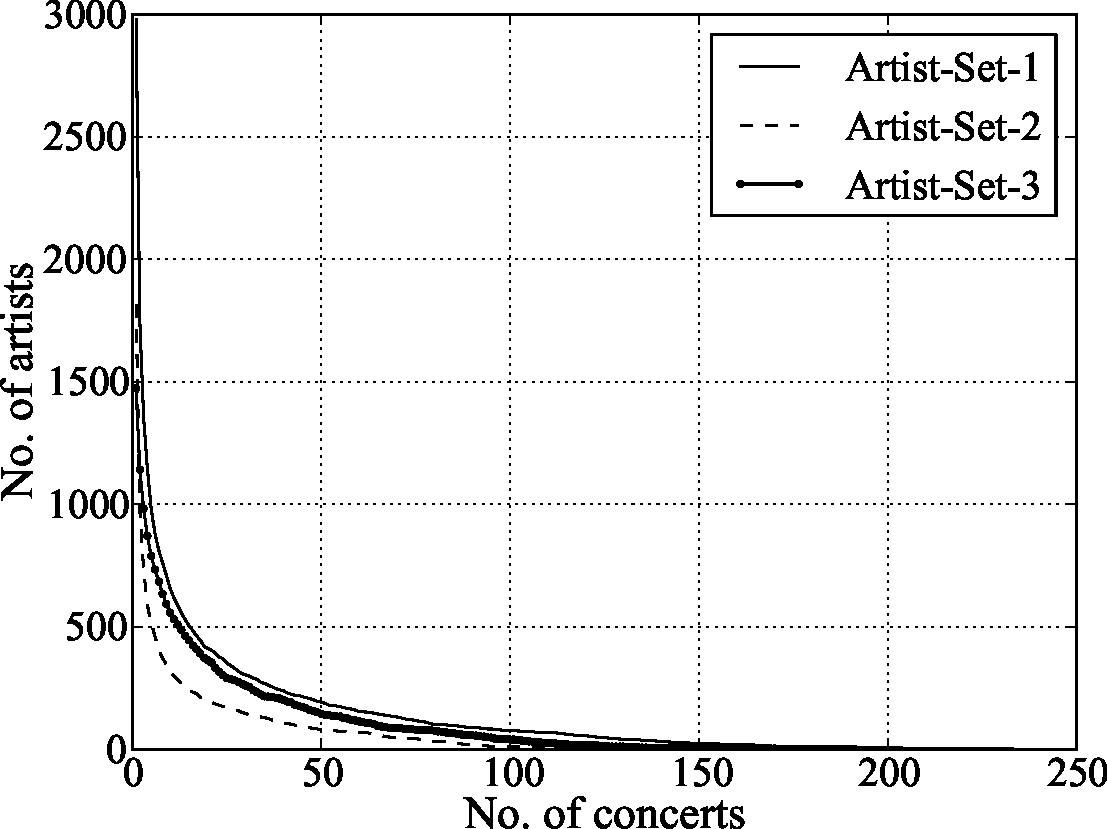
\includegraphics[width=\textwidth]{./figs/dstats/performances-vs-artists.pdf}
\caption{The number of artists by the number of their performances in the Carnatic music research corpus}
\label{fig:corpora:perfArtistDistr}
\end{figure}
%
\begin{figure}[t]
\centering
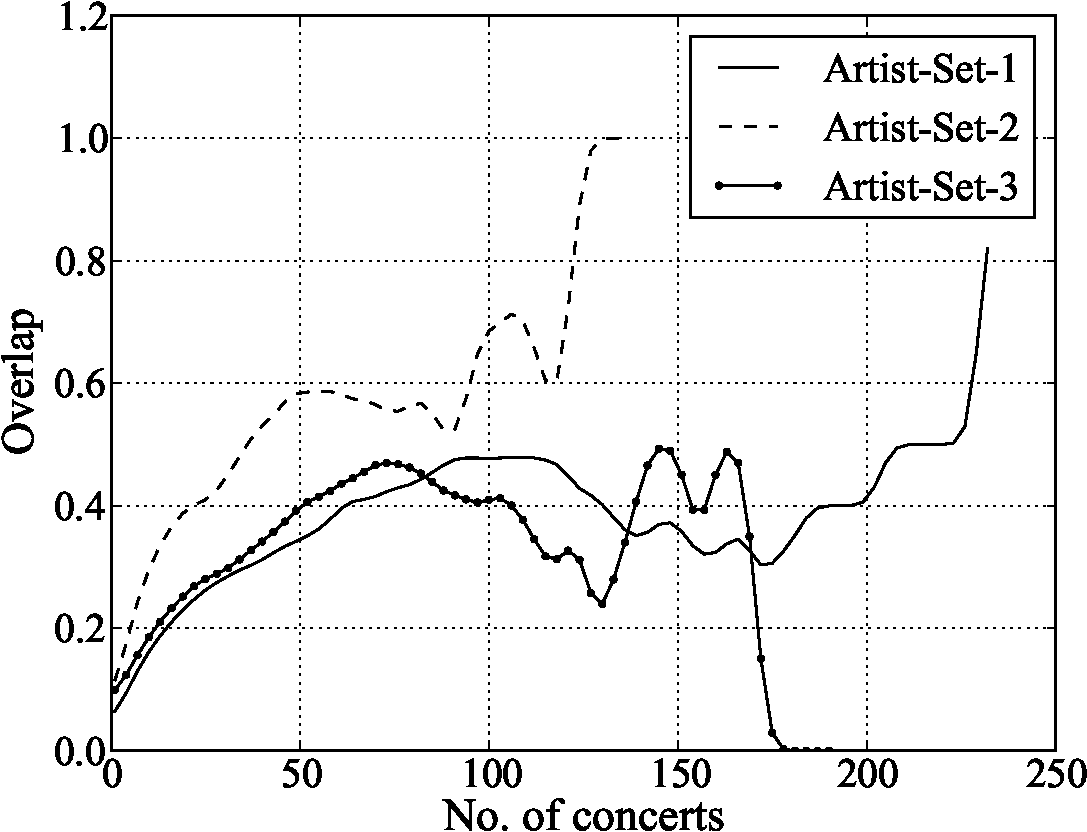
\includegraphics[scale=0.6]{./figs/dstats/artist-coverage-vs-performances.pdf}
\caption[Coverage of the Carnatic artists]{Coverage of Carnatic artists. The ordinate is the \textit{overlap} value of the set of artists in corpus, compared against a set of artists in Kutcheris.com who have performed in at least as many concerts as the abscissa.}
\label{fig:corpora:artistCoverage}
\end{figure}

\tabref{tab:coverage:Carnatic} shows the coverage of the Carnatic corpus in comparison to the references. For each music entity $i$, we define a coverage measure called the \textit{overlap} (\ovlp) as,
\begin{equation}
\label{eqn:overlap}
\ovlp_i^j = \frac{\left| \varsigma_i^c \cap \varsigma_i^j\right|}{\left|\varsigma_i^j\right|}
\end{equation}
where $\ovlp_i^j$ is the \textit{overlap} measure of the entity $i$ with reference $j$, $\varsigma_i^c$ is the set of entities in the corpus, $\varsigma_i^j$ is the set of entities in the reference, and $\left| \varsigma \right|$ denotes the cardinality of a set $\varsigma$. An \textit{overlap} of 100\% is achieved if all the elements in the reference set are present in the corpus. \tabref{tab:coverage:Carnatic} shows the \textit{overlap} measure for \glspl{raga}, \glspl{tala} and composers for both Raaga.com and Charsur. We can see that there is a good coverage of \glspl{tala} and a satisfactory coverage of \glspl{raga} in the corpus. A good coverage of \glspl{tala} is necessary for rhythm analysis. The composer coverage with respect to Raaga.com is poor since it includes the light music composers in its set of composers. 

Among the 233 artists who have at least one recording in the corpus, 74 are lead artists (lead vocal or lead instrumental). Further, we have 28 violin accompanying artists and 48 unique percussion artists in the corpus. The concerts listed by Kutcheris.com span the whole year and all through the day. However, the evening concerts are more recognized, and we took it to be a measure of popularity of the artists. Moreover, the evening concerts during the music season lasting from November to January are ticketed. For a coverage analysis, we thus consider three categories of artists: Artists-Set-1 (all the artists), Artists-Set-2 (artists who have performed in the evening concerts, through the year) and Artists-Set-3 (artists who have performed in evening concerts between November and January). Of the 2978 total artists present in Set-1 on Kutcheris.com concert listings, there are 1814 artists in Set-2 and 1472 artists in Set-3.

The number of concerts performed by each artist is also an indicator of popularity. Though there are a large number of artists in Kutcheris, we see that the distribution of the number of concerts they have performed is exponential (\figref{fig:corpora:perfArtistDistr}), e.g. there are only about 200 artists who have over 50 concerts. Hence to capture this fact, we used the set of artists in the corpus and computed the \textit{overlap} as defined in \eqnref{eqn:overlap} through different subsets of artists in Kutcheris.com, sweeping over the number of concerts (at least) they have performed. 

\figref{fig:corpora:artistCoverage} shows the \textit{overlap}, using a set of artists that have performed at least as many concerts as the number shown on the abscissa. The \textit{overlap} is also shown for the three categories of artists we discussed before. We can see that the \textit{overlap} increases as we consider more frequently performing artists and becomes almost constant. The artists who have performed the most concerts are often the accompanying artists, and are few in number, which explains why the \textit{overlap} becomes a constant, when we discount the \textit{overlap} for more than 150 concerts. When we consider a large number of concerts, the \textit{overlap} values are unreliable since the number of artists is less. In general, we can see that the \textit{overlap} is better for Artists-Set-2 than Artists-Set-1 and Artists-Set-3, showing that the corpus has more representation of artists from evening concerts round the year. 
% 
\subsubsection{Completeness}
\begin{table}
\begin{centering}
\begin{tabular}{@{}lcr@{}}
\toprule 
\textbf{Accompanying metadata} & \textbf{\#Recordings} & \textbf{\% of total}\tabularnewline
\midrule 
Lead artist & 1650 & 100.0 \tabularnewline
Accompanying artists& 1221 & 74.0\tabularnewline
\Gls{raga} & 959 & 58.1\tabularnewline
\Gls{tala} & 917 & 55.6\tabularnewline
Work (Composition) & 989 & 59.9\tabularnewline
\bottomrule 
\end{tabular}
\par\end{centering}
\caption[Completeness of the Carnatic music research corpus]{Completeness of the Carnatic music research corpus, showing the number of recordings in which the corresponding metadata is available.}\label{tab:completeness:Carnatic}
\end{table}
In the context of this thesis, completeness of the corpus refers mainly to the completeness of the associated metadata for each recording, primarily from MusicBrainz. Even though carefully built, the editorial metadata associated with a release and its recordings can be incomplete. There are three possible reasons for incomplete metadata. Many releases do not provide all the required metadata on the CD. In many releases, only the lead artist is listed, without the accompanying artists. It is seen very often that the composition information is also absent on the CD cover. The second reason is that the editorial metadata was not completely entered into MusicBrainz. This is sometimes seen with release and recording relationships that were left incomplete by the person who added the metadata. Further, since all the metadata, including the \gls{raga}/\gls{tala} tags, are imported and linked automatically, there can be import errors due to variations in transliterations and spelling. Multiplicity of languages used in Carnatic music further adds to these inconsistencies. These import errors are the third reason for incomplete metadata. 

Missing metadata in MusicBrainz can only be completed by manually adding the missing fields to MusicBrainz. However, we are also exploring automatic metadata completion based on other relations on the release or the recording, using semantic web approaches. The missing data due to transliteration errors have been addressed to an extent by making curated lists of entities such as \glspl{raga} and \glspl{tala}, and using robust algorithms for matching and linking metadata. Despite significant efforts, there are many recordings and releases that have incomplete metadata. 

\tabref{tab:completeness:Carnatic} shows the completeness of the recordings in the corpus (as of June 2014), including all the three factors that result in incomplete metadata. All the recordings have a lead artist, but about a quarter of the recordings (429/1650) do not have accompanying artist information. \Gls{raga}, \gls{tala} and work (composition) are listed for about half the recordings. It is to be noted that these numbers reflect only the recordings for which we were completely sure of the editorial metadata. There are several recordings that have the required metadata but deemed incomplete since we could not accurately match it to a related entity in the curated lists. 
%
\subsection{Hindustani music research corpus}\label{sec:cmhmcorpora}
%* Provide statistics and discuss: Purpose, Coverage, Completeness, Quality, Reusability
%* Contents: Audio, MB metadata, lyrics, reference books
%<<Intro and contents>>
%<<Considerations>>
Similar to Carnatic music, \gls{raag} and \gls{taal} are the fundamental music concepts in Hindustani music\index{Hindustani music} and hence the main theme around which the corpus has been built. Hindustani music tradition is much more diverse and heterogeneous and thus presents a significant challenge to compile a good research corpus. Though vocal music is predominant, instrumental music in Hindustani music is also popular. The main focus in Hindustani music is on improvisation and compositions are short. For Hindustani music corpus we focus on two important vocal music styles - \gls{dhrupad} and \gls{khayal}. 

There are many public and private institutions that have compiled large audio archives of Hindustani music. The primary of them are the ITC Sangeet Research Academy (ITC-SRA), Sangeet Natak Academy, and the All India Radio (AIR). Each of these institutions own thousands of hours of expert curated music recordings that represent the real world performance practice. 

ITC-SRA is a premier music academy of Hindustani music and has taken up major efforts in the archival of music. Sangeet Natak Academy is India's national academy for music, drama and dance. AIR is the largest public broadcaster in India and has a huge archive of Hindustani music curated over many decades. AIR awards grades to musicians and its archives can be considered as a reference. None of these archives are publicly available and we compiled the audio in our corpus using these collections as a reference. We consulted expert musicians and musicologists, such as Dr. Suvarnalata Rao at the National Centre for the Performing Arts (NCPA), Mumbai, India to curate the audio collection in the corpus. 

The audio collection in the corpus comprises commercially available music releases from several music labels. It mainly consists of \gls{khayal} and \gls{dhrupad} vocal music releases, though a significant number of instrumental music releases are present. The corpus presently has 233 releases with a total of 1096 recordings (300 hours). As with Carnatic music, the editorial metadata associated with each release is stored in MusicBrainz. 

The metadata associated with each release is the name of the release, the lead and the accompanying artists, and the musical instruments in the concert. For each audio recording in the release, the relevant metadata are the artists performed on the track, the name of the composition/s (\gls{bandish}) and the composer/s (if composed), \gls{raag}/s, \gls{taal}/s, \gls{lay}/s (tempo class), form/s, and section/s. All the editorial metadata was entered using Latin alphabet, following a uniform transliteration scheme to maintain consistency. 

%<<Lyrics and Score>>
Hindustani music is mainly improvised and hence lyrics and scores are not very relevant for computational analysis. \citeA{bhatkhande:90:book} and \citeA{jha:01:book} compiled lyrics and scores of \glspl{bandish} using a standardized notation for Hindustani music. However, they are not available in a machine readable form, though a small collection of scores from these books are available in machine readable Humdrum format~\cite{ajay:12:humdrum}. Swarganga Music Foundation\footnote{\url{http://www.swarganga.org/}} has a good archive of \glspl{raag}, \glspl{taal} and \glspl{bandish}. The category of Hindustani music on Wikipedia\footnote{\url{http://en.wikipedia.org/wiki/Category:Hindustani_music}} is a source of contextual information including music concepts of Hindustani music. 
%<<Coverage analysis>>
\begin{table}[t]
\begin{centering}
\begin{tabular}{@{}lrll@{}}
\toprule 
 & \textbf{Corpus} & \textbf{ITC-SRA} & \textbf{Swarganga}\tabularnewline
\midrule 
Artists & 360 & 240 (19\%) & 629 (14\%)\tabularnewline
\Glspl{raag} & 176 & 185 (48\%) & 534 (13\%)\tabularnewline
\Glspl{taal} & 32 & N/A & \ \ 59 (37\%)\tabularnewline
Works (\Gls{bandish}) & 685 & N/A & 1957\tabularnewline
\bottomrule 
\end{tabular}
\par\end{centering}
\caption[Coverage of the Hindustani music research corpus]{Coverage of the Hindustani music research corpus. The number in parentheses is the \textit{overlap} measure in percentage. N/A indicates data not available.}\label{tab:coverage:Hindustani}
\end{table}
\begin{table}[t]
\begin{centering}
\begin{tabular}{@{}lcr@{}}
\toprule
\textbf{Accompanying metadata} & \textbf{\# Recordings} & \textbf{\% of total}\tabularnewline
\midrule
Lead Artist & 1096 & 100.0\tabularnewline
Accompanying artist  & 658 & 60.0\tabularnewline
\Gls{raag} & 960 & 87.6\tabularnewline
\Gls{taal} & 627 & 57.2\tabularnewline
Work (\Gls{bandish}) & 576 & 52.5\tabularnewline
\bottomrule 
\end{tabular}
\par\end{centering}
\caption[Completeness of the Hindustani music research corpus]{Completeness of the Hindustani music research corpus showing the number of recordings in which the corresponding metadata is available.}\label{tab:completeness:Hindustani}
\end{table}
\subsubsection{Coverage}
The methodology followed for the coverage analysis of Hindustani music is the same as followed for Carnatic music. We present the coverage analysis for artists, \glspl{raag}, \glspl{taal} and compositions. The coverage analysis for Hindustani music is more complex than Carnatic music. This can be attributed to the heterogenous nature of the music repertoire, and to the lack of dedicated recording labels like Charsur in the case of Carnatic music. For each of these entities we choose two main references, ITC-SRA and Swarganga. 

Unlike Carnatic music, the unit of music distribution in Hindustani music is not often a concert. Further, it is geographically spread over the Indian subcontinent and hence there is no single repository of Hindustani music performances, such as Kutcheris.com for Carnatic music. Therefore, it is challenging to do a comprehensive artist coverage analysis like the one presented for Carnatic music. 

\tabref{tab:coverage:Hindustani} shows the coverage of the Hindustani corpus. We see that the corpus and the chosen references have comparable number of entities, but the \textit{overlap} is less. This is primarily because we mainly focused on recordings made in last 20-30 years to ensure good recording quality and to reflect current performance practices. On the other hand both the references focus primarily on archiving Hindustani music and hence consist of several generations of artists, infrequent \glspl{raag} and \glspl{taal}, and a more comprehensive list of compositions. Further, the Hindustani corpus is mainly composed of vocal music recordings with a focus on only two styles, \gls{khayal} and \gls{dhrupad}. The reference archives additionally include instrumental music and several other styles of Hindustani music. 
\subsubsection{Completeness}
The completeness of the editorial metadata for Hindustani music (as of June 2014) is shown in \tabref{tab:completeness:Hindustani}. We see that the editorial metadata for all the recordings at least includes the lead artist, and for more than half of the collection, the accompanying artists (658/1096). Roughly 90\% of the corpora is annotated with the \gls{raag} label and more than half with the \gls{taal} label. Work or compositions (\gls{bandish}) labels are present for nearly half of the collection (576/1096). \Gls{alap} performances in Hindustani music are not compositional works, and hence should be discounted while assessing the completeness of work metadata. But due to the unavailability of such an information (\gls{alap} labels), \gls{alap} performances are also included in assessment and hence work completeness is an underestimate. 
%%%%%%%%%%%%%%%%%%%%%%%%%%%%%%%%%%%

%\comment{Since we have addressed coverage and completeness later on, here is reproducibility} 
An important concern in research is the reproducibility of the experiments, which necessitates a corpus accessible to the research community. When possible, we emphasize the use of open repositories of information such as MusicBrainz and Wikipedia. The releases in the Carnatic\footnote{Carnatic collection: \url{http://musicbrainz.org/collection/f96e7215-b2bd-4962-b8c9-2b40c17a1ec6}} and Hindustani\footnote{Hindustani collection: \url{http://musicbrainz.org/collection/213347a9-e786-4297-8551-d61788c85c80}} corpora have been organized into collections in MusicBrainz. For audio, we use easily accessible commercial recordings. Further, the test datasets and the derived information such as annotations and extracted features are openly available\footnote{CompMUsic corpora: \url{http://compmusic.upf.edu/corpora}}. In CompMusic, have developed a tool for navigating through music collections called \textit{Dunya}~\cite{porter:13:dunya}, which also acts as the central permanent online repository to store the metadata, audio, annotations and research results. Dunya is open source and provides an API for accessing these data. 
%
%\comment{Dunya collection and possible work with it: All the applications of the corpus, list, explain, and cite}
\subsection{Creative Commons music collections}\label{sec:cmccdataset}
The audio in the Carnatic and Hindustani research corpora are commercial releases. Though easily accessible, they cannot be distributed openly. Since there are no open repositories of quality audio, one effort of CompMusic is to create and open audio collection released under Creative Commons licenses (CC BY-NC 4.0). In addition to the audio, the collection has carefully curated editorial metadata, and semi-automatically extracted melody and rhythm related annotations. Due permissions from artists have been secured for redistribution. The audio will be hosted on Internet Archive\footnote{\url{www.archive.org}}, with both the audio and associated metadata and annotations available through the Dunya API. The open music collections are growing collections with new releases being added, and hence the numbers in this section (correct as of June 2016) are approximate and indicative.

The \acrfull{CMDo}\footnote{Carnatic CC collection: \url{https://musicbrainz.org/collection/a163c8f2-b75f-4655-86be-1504ea2944c2}} is a collection of 20 vocal Carnatic concerts (with more releases being added) with 197 tracks and over 41 hours of music by professional Carnatic musicians. The audio in the \acrshort{CMDo} collection was professionally recorded in multi-track at 44.1kHz sampling rate at Arkay Convention Center, Chennai, India, and mastered professionally. The pieces from the concerts were split into individual recordings and released together as an album. Each recording has the following accompanying metadata: \gls{raga}, \gls{tala}, artists, composer, composition, and form. It has manually annotated time aligned characteristic melodic phrases and sections. In addition, it has semi-automatically extracted tonic, vocal pitch track, tempo, and time aligned \gls{sama} annotations. The collection has about 16880 \gls{sama} annotations that can be used for meter analysis.

The \acrfull{HMDo}\footnote{Hindustani CC collection: \url{https://musicbrainz.org/collection/6adc54c6-6605-4e57-8230-b85f1de5be2b}} is a collection of 36 vocal Hindustani music albums (with more releases being added) with 108 tracks and over 43 hours of music by professional Hindustani musicians, sourced from personal collections of musicians. The audio in the \acrshort{HMDo} collection are stereo mp3 tracks sampled at 44.1 kHz. The tracks procured from personal collections have been grouped into musically meaningful short compilations and then released as albums. Each recording in the collection has the following accompanying metadata: \gls{raag}, \gls{taal}, \gls{lay}/s, artists, form, and if applicable, the \gls{bandish} and the composer. It has manually annotated time aligned characteristic melodic phrases and \gls{lay} based sections. In addition, it has semi-automatically extracted tonic, vocal pitch track, tempo, and time aligned \gls{sam} annotations. The collection has about 11260 \gls{sam} annotations that can be used for meter analysis. 

The Creative Commons collections are useful for several \gls{MIR} tasks. From a rhythm analysis perspective, the collection is useful for meter inference and tracking, rhythmic and percussion pattern analysis, and rhythm based structural segmentation. To the best of our knowledge, this collection is the largest \gls{tala} and \gls{sama} annotated music collection of Indian art music. 
\section{Test datasets}
%\comment{For each dataset below, present a basic statistical analysis, links to download. Mention which tasks they are the most useful for. The limitations of the dataset and what can be improved as well.}
The test corpora (or test datasets)\index{Test dataset} are designed for specific tasks and contain additional information such as annotations and derived data. They are useful for various melody and rhythm analysis tasks. There are several test datasets for different music cultures built within CompMusic\footnote{\url{http://compmusic.upf.edu/datasets}}, while we describe only those test datasets that are useful in rhythm analysis tasks. We describe each dataset briefly emphasizing the primary research task they can be used for. 
\subsection{Carnatic music rhythm dataset}\label{sec:cmrdataset}
%% CMDF table of dataset
The \acrfull{CMDf}\footnote{\url{http://compmusic.upf.edu/carnatic-rhythm-dataset}}\index{Carnatic music} is a rhythm annotated test corpus for many automatic rhythm analysis tasks in Carnatic Music~\cite{ajay:14:talaTrack}. The dataset consists of audio excerpts from the Carnatic research corpus, manually annotated time-aligned markers indicating the progression through the \gls{tala} cycle, and the associated \gls{tala} related metadata. 
\begin{table}[t]
\begin{center}
\tabcolsep=0.12cm
\begin{tabular}{@{}lrccrr@{}}
\toprule 
\Gls{tala} & \#Pieces & Total Duration & $\overline{\songlen}$ & \#Ann. & \#Sama\tabularnewline
 &  & hours (min) &  &  & \tabularnewline
\midrule 
\Gls{adi} & 50 & 4.21 (252.78) & 4m51s & 22793 & 2882\tabularnewline
\Gls{rupaka} & 50 & 4.45 (267.45) & 4m37s & 22668 & 7582\tabularnewline
\Gls{mishra chapu} & 48 & 5.70 (342.13) & 6m35s & 54309 & 7795\tabularnewline
\Gls{khanda chapu} & 28 & 2.24 (134.62) & 4m25s & 21382 & 4387\tabularnewline
\midrule 
Total & 176 & 16.61 (996.98) & 5m4s & 121602 & 22646\tabularnewline
\bottomrule 
\end{tabular}
\end{center}
\protect\caption[\acrshort{CMDf} dataset description]{\acrshort{CMDf} dataset showing the total duration and number of annotations. \#Sama shows the number of \gls{sama} annotations and \#Ann. shows the number of beat annotations (including \glspl{sama}). $\protect\overline{\protect\songlen}$ indicates the median piece length in the dataset (m and s indicate minutes and seconds, respectively)}
\label{tab:dataset:cmdf}
\end{table}
%% CMDF table of datastats
\begin{table}[t]
\centering
\begin{tabular}{@{}lccc@{}}
\toprule 
\Gls{tala} & $\overline{\isi} \pm \sigma_s$ & $\overline{\iai} \pm \sigma_o$ & $[{\isi}_{,\min} \, , \,  {\isi}_{,\max} ]$ \tabularnewline
\midrule 
\Gls{adi}  & 5.34 $\pm$ 0.723 & 0.167 $\pm$ 0.023 & $[$2.88, 7.07$]$\tabularnewline
\Gls{rupaka} & 2.13 $\pm$ 0.239 & 0.178 $\pm$ 0.020 & $[$1.21, 3.10$]$\tabularnewline
\Gls{mishra chapu} & 2.67 $\pm$ 0.358 & 0.191 $\pm$ 0.026 & $[$1.63, 3.65$]$\tabularnewline
\Gls{khanda chapu} & 1.85 $\pm$ 0.284 & 0.185 $\pm$ 0.028 & $[$0.91, 2.87$]$\tabularnewline
\bottomrule 
\end{tabular}
\protect\caption[\Gls{tala} cycle length indicators for \acrshort{CMDf} dataset]{\Gls{tala} cycle length indicators for \acrshort{CMDf} dataset. $\overline{\isi}$ and $\sigma_s$ indicate the mean and standard deviation of the median inter-\gls{sama} interval of the pieces, respectively. $\overline{\iai}$ and $\sigma_o$ indicate the mean and standard deviation of the median inter-\gls{akshara} interval of the pieces, respectively. $[{\isi}_{,\min} \, , \,  {\isi}_{,\max} ]$ indicate the minimum and maximum value of $\isi$ and hence the range of $\isi$ in the dataset. All values in the table are in seconds.}
\label{tab:datastat:cmdf}
\end{table}

\acrshort{CMDf} dataset is described in \tabref{tab:dataset:cmdf}, showing the four \glspl{tala} and the number of pieces for each \gls{tala}. The dataset has pieces in four popular \glspl{tala} that encompass a majority of current day Carnatic music performance. The pieces include a mix of vocal and instrumental recordings, recent and old recordings, and span a wide variety of forms. All pieces have a percussion accompaniment, predominantly mridangam. There are also several different pieces by the same artist (or release group), and multiple instances of the same composition rendered by different artists. Each piece is uniquely identified using the \gls{MBID} of the recording. The pieces are mp3 stereo recordings, and sampled at 44.1 kHz. The audio is also available as downmixed mono WAV files for experiments. The audio files are full length pieces or clips extracted from full length pieces. Of the 176 audio files, 120 contain full length pieces. 

There are several annotations that accompany each excerpt in the dataset. The primary annotations are audio synchronized time-stamps indicating the different metrical positions in the \gls{tala} cycle - the \gls{sama} (downbeat) and other beats shown with numerals in \figref{fig:taala:carnatic}. The annotations were created using Sonic Visualizer~\cite{cannam:10:sv} by tapping to music and manually correcting the taps. The annotations have been verified by a professional Carnatic musician. Each annotation has a time-stamp and an associated numeric label that indicates the position of the beat marker in the \gls{tala} cycle. In addition, for each excerpt, the \gls{tala} of the piece and \gls{edupu} (offset of the start of the piece, relative to the sama) are recorded. The possibly time varying tempo of a piece can be obtained using the beat and \gls{sama} annotations. 
%% CMD table of dataset
\begin{table}[t]
\centering
\begin{tabular}{@{}lrcrr@{}}
\toprule 
\Gls{tala} & \# Pieces & Total Duration & \# Ann. & \# Sama\tabularnewline
 &  & hours (min) &  & \tabularnewline
\midrule 
\Gls{adi} & 30 & 0.98 (58.87) & 5452 & 696\tabularnewline
\Gls{rupaka} & 30 & 1.00 (60.00) & 5148 & 1725\tabularnewline
\Gls{mishra chapu} & 30 & 1.00 (60.00) & 8992 & 1299\tabularnewline
\Gls{khanda chapu} & 28 & 0.93 (55.93) & 9133 & 1840\tabularnewline
\midrule 
Total & 118 & 3.91 (234.80) & 28725 & 5560\tabularnewline
\bottomrule 
\end{tabular}
\protect\caption[\acrshort{CMDs} dataset description]{\acrshort{CMDs} dataset showing the total duration and number of annotations. \#Sama shows the number of \gls{sama} annotations and \#Ann. shows the number of beat annotations (including \glspl{sama}).}
\label{tab:dataset:cmd}
\end{table}
%
%% CMD table of datastats
\begin{table}[t]
\centering
\begin{tabular}{@{}lccc@{}}
\toprule 
\Gls{tala} & $\overline{\isi} \pm \sigma_s$ & $\overline{\iai} \pm \sigma_o$ & $[{\isi}_{,\min} \, , \,  {\isi}_{,\max} ]$ \tabularnewline
\midrule 
\Gls{adi} & 5.32 $\pm$ 0.868 & 0.17 $\pm$ 0.027 & {[}2.88, 7.07{]}\tabularnewline
\Gls{rupaka} & 2.12 $\pm$ 0.225 & 0.18 $\pm$ 0.019 & {[}1.40, 3.10{]}\tabularnewline
\Gls{mishra chapu} & 2.81 $\pm$ 0.272  & 0.20 $\pm$ 0.019  & {[}2.03, 3.65{]}\tabularnewline
\Gls{khanda chapu} & 1.87 $\pm$ 0.290 & 0.19 $\pm$ 0.029 & {[}1.00, 2.84{]}\tabularnewline
\bottomrule 
\end{tabular}
\protect\caption[\Gls{tala} cycle length indicators for \acrshort{CMDs} dataset]{\Gls{tala} cycle length indicators for \acrshort{CMDs} dataset. $\overline{\isi}$ and $\sigma_s$ indicate the mean and standard deviation of the median inter-\gls{sama} interval of the pieces, respectively. $\overline{\iai}$ and $\sigma_o$ indicate the mean and standard deviation of the median inter-\gls{akshara} interval of the pieces, respectively. $[{\isi}_{,\min} \, , \,  {\isi}_{,\max}]$ indicate the minimum and maximum value of $\isi$ and hence the range of $\isi$ in the dataset. All values in the table are in seconds.}
\label{tab:datastat:cmd}
\end{table}

The total duration of audio in the dataset is over 16.6 hours, with 121062 time-aligned beat annotations. The median length of a piece is about 5 minutes in the dataset. \tabref{tab:datastat:cmdf} shows a basic statistical analysis of the \gls{tala} cycle length indicators in the dataset, which is useful to understand the tempo characteristics and the range of the metrical cycle lengths in the dataset. \Gls{adi} \gls{tala} is the longest \gls{tala} in the dataset and hence has the highest $\overline{\isi}$ among all the \glspl{tala}. Despite no notated tempo, we can see from the values of the median inter-\gls{akshara} interval, $\overline{\iai}$ and its standard deviation that the tempo in Carnatic music does not vary much across the \glspl{tala}. The range of $\overline{\isi}$ values show that a wide range of cycle durations that are present in Carnatic music pieces. The shortest cycle in the dataset is less than second long, while the longest cycle is over 7 seconds long. % spanning three tempo octaves. (, which means that we need more robust methods to handle tempo octave errors in tempo estimation.)The range of $\overline{\isi}$ values show that a wide range of tempi are present in Carnatic music pieces, often over two tempo octaves.
% Dataset stats: CMDf-ISI
\begin{figure}[t]
\centering
\subfloat[\Gls{adi}]{\label{fig:dstats:CMDf:ISI:adi}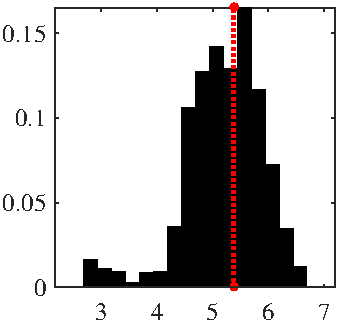
\includegraphics[scale=0.9]{dstats/CMDf-adi-ISI.pdf}} \hspace{0.5cm} 
\subfloat[\Gls{rupaka}]{\label{fig:dstats:CMDf:ISI:rupaka}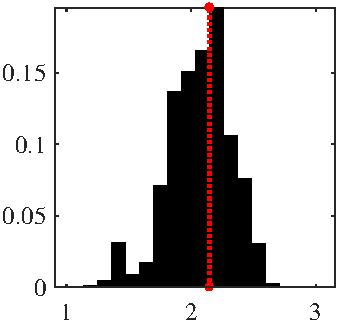
\includegraphics[scale=0.9]{dstats/CMDf-rupaka-ISI.pdf}} \\ 
\subfloat[\Gls{mishra chapu}]{\label{fig:dstats:CMDf:ISI:mishraChapu}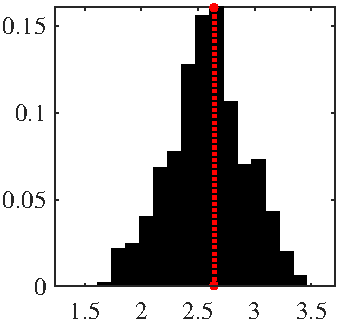
\includegraphics[scale=0.9]{dstats/CMDf-mishraChapu-ISI.pdf}} \hspace{0.5cm} 
\subfloat[\Gls{khanda chapu}]{\label{fig:dstats:CMDf:ISI:khandaChapu}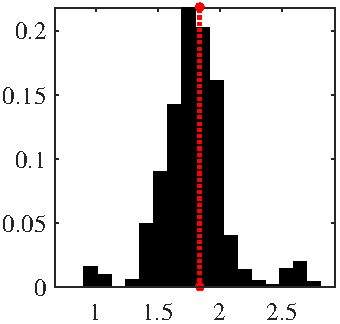
\includegraphics[scale=0.9]{dstats/CMDf-khandaChapu-ISI.pdf}} \\ 
\caption[Histogram of $\protect\isi$ in the \acrshort{CMDf} dataset]{A histogram of the inter-\gls{sama} interval $\protect\isi$ in the \acrshort{CMDf} dataset for each \gls{tala}. The ordinate is the fraction of the total count corresponding to the $\isi$ value shown in abscissa. The median $\isi$ for each \gls{tala} is shown as a red dotted line.}\label{fig:dstats:CMDf:ISI}
\end{figure}
% Dataset stats: CMDf-IAI
\begin{figure}[t]
\centering
\subfloat[\Gls{adi}]{\label{fig:dstats:CMDf:IAI:adi}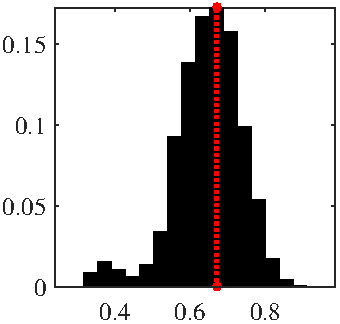
\includegraphics[scale=0.9]{dstats/CMDf-adi-IAI.pdf}} \hspace{0.5cm} 
\subfloat[\Gls{rupaka}]{\label{fig:dstats:CMDf:IAI:rupaka}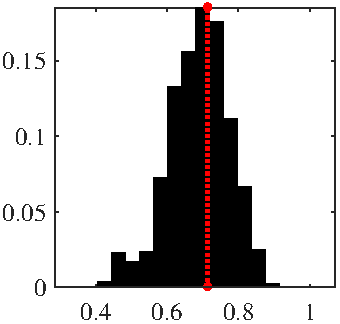
\includegraphics[scale=0.9]{dstats/CMDf-rupaka-IAI.pdf}} \\ 
\subfloat[\Gls{mishra chapu}]{\label{fig:dstats:CMDf:IAI:mishraChapu}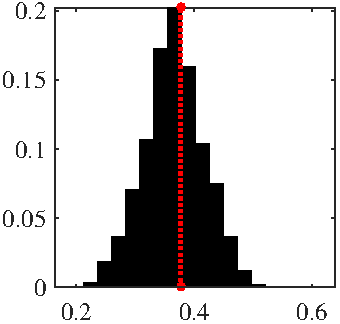
\includegraphics[scale=0.9]{dstats/CMDf-mishraChapu-IAI.pdf}} \hspace{0.5cm} 
\subfloat[\Gls{khanda chapu}]{\label{fig:dstats:CMDf:IAI:khandaChapu}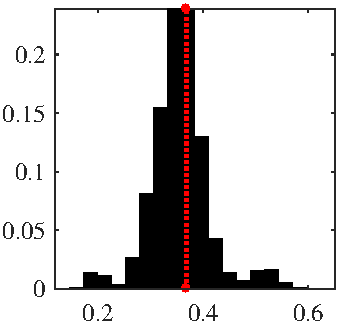
\includegraphics[scale=0.9]{dstats/CMDf-khandaChapu-IAI.pdf}} \\ 
\caption[Histogram of $\protect\ibi$ in the \acrshort{CMDf} dataset]{A histogram of the inter-beat interval $\protect\ibi$ in the \acrshort{CMDf} dataset for each \gls{tala}. The ordinate is the fraction of the total count corresponding to the $\ibi$ value shown in abscissa. The median $\ibi$ for each \gls{tala} is shown as a red dotted line.}\label{fig:dstats:CMDf:IAI}
\end{figure}
%
% Dataset stats: CMDf-ISInorm
\begin{figure}
%\captionsetup[subfigure]{labelformat=empty}
\begin{center}
\subfloat[\Gls{adi}]{\label{fig:dstats:CMDf:ISInorm:adi}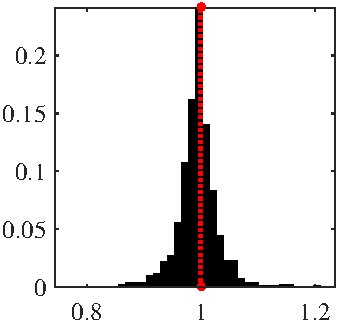
\includegraphics[scale=0.9]{dstats/CMDf-adi-ISInorm.pdf}} \hspace{0.5cm} 
\subfloat[\Gls{rupaka}]{\label{fig:dstats:CMDf:ISInorm:rupaka}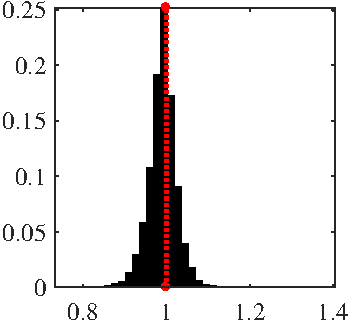
\includegraphics[scale=0.9]{dstats/CMDf-rupaka-ISInorm.pdf}} \\ 
\subfloat[\Gls{mishra chapu}]{\label{fig:dstats:CMDf:ISInorm:mishraChapu}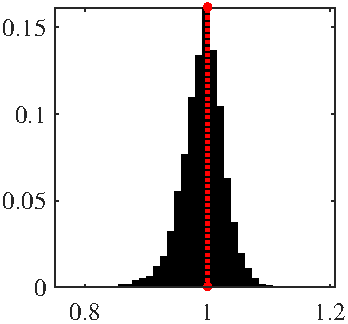
\includegraphics[scale=0.9]{dstats/CMDf-mishraChapu-ISInorm.pdf}} \hspace{0.5cm} 
\subfloat[\Gls{khanda chapu}]{\label{fig:dstats:CMDf:ISInorm:khandaChapu}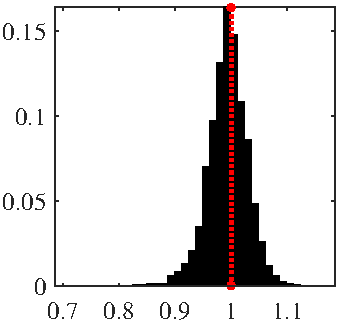
\includegraphics[scale=0.9]{dstats/CMDf-khandaChapu-ISInorm.pdf}} \\ 
\caption[Histogram of median normalized $\protect\isi$ in the \acrshort{CMDf} dataset]{A histogram of the median normalized inter-\gls{sama} interval $\protect\isi$ in the \acrshort{CMDf} dataset for each \gls{tala}. The ordinate is the fraction of the total count corresponding to the normalized $\isi$ value shown in abscissa.}\label{fig:dstats:CMDf:ISInorm}
\end{center}
\end{figure}
%
% Dataset stats: CMDf-IAInorm
\begin{figure}
%\captionsetup[subfigure]{labelformat=empty}
\begin{center}
\subfloat[\Gls{adi}]{\label{fig:dstats:CMDf:IAInorm:adi}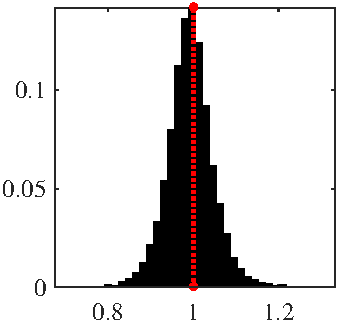
\includegraphics[scale=0.9]{dstats/CMDf-adi-IAInorm.pdf}} \hspace{0.5cm} 
\subfloat[\Gls{rupaka}]{\label{fig:dstats:CMDf:IAInorm:rupaka}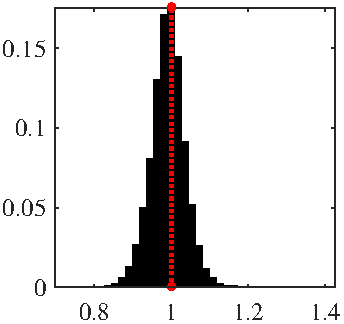
\includegraphics[scale=0.9]{dstats/CMDf-rupaka-IAInorm.pdf}} \\ 
\subfloat[\Gls{mishra chapu}]{\label{fig:dstats:CMDf:IAInorm:mishraChapu}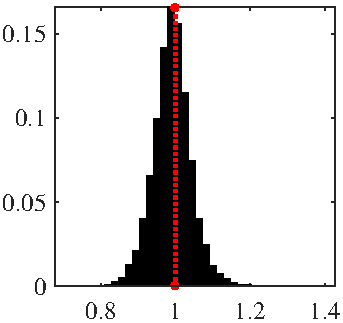
\includegraphics[scale=0.9]{dstats/CMDf-mishraChapu-IAInorm.pdf}} \hspace{0.5cm} 
\subfloat[\Gls{khanda chapu}]{\label{fig:dstats:CMDf:IAInorm:khandaChapu}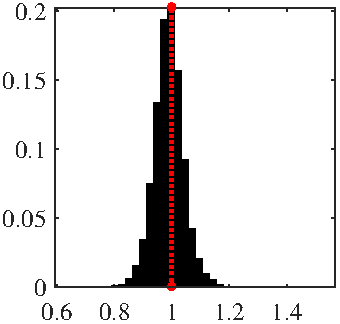
\includegraphics[scale=0.9]{dstats/CMDf-khandaChapu-IAInorm.pdf}} \\ 
\caption[Histogram of median normalized $\protect\ibi$ in the \acrshort{CMDf} dataset]{A histogram of the median normalized inter-beat interval $\protect\ibi$ in the \acrshort{CMDf} dataset for each \gls{tala}. The ordinate is the fraction of the total count corresponding to the normalized $\ibi$ value shown in abscissa.}\label{fig:dstats:CMDf:IAInorm}
\end{center}
\end{figure}

A representative subset of the \acrshort{CMDf} dataset is also compiled as the \acrshort{CMDs} dataset, with two minute excerpts of pieces in \acrshort{CMDf} (or the full piece if the piece is shorter than 2 minutes). These short excerpts additionally contain all the annotations of the full dataset, including time aligned \gls{sama} and beat annotations. The smaller \acrshort{CMDs} dataset will be useful for faster testing of approaches and algorithms. 

The \acrshort{CMDs} dataset is described in \tabref{tab:dataset:cmd}, showing the four \glspl{tala} and the number of pieces for each \gls{tala}. The total duration of audio in the dataset is about 4 hours, with 28725 time-aligned beat annotations. \tabref{tab:datastat:cmd} shows a basic statistical analysis of the \gls{tala} cycle length indicators in the \acrshort{CMDs} dataset, which are similar to the indicators of \acrshort{CMDf} dataset shown in \tabref{tab:datastat:cmdf}, showing that \acrshort{CMDs} dataset is a representative subset of \acrshort{CMDf} dataset. 

The tempo values are not notated in Carnatic music, and the pieces are not played to a metronome. Hence, in addition to the median values tabulated in \tabref{tab:datastat:cmdf} we present further analysis of the inter-\gls{sama} interval (\isi) and inter-beat interval (\ibi) for each \gls{tala} over the whole \acrshort{CMDf} dataset. A histogram of $\isi$ and $\ibi$ for each \gls{tala} is shown in \figref{fig:dstats:CMDf:ISI} and \figref{fig:dstats:CMDf:IAI} respectively. This shows the distribution of cycle lengths in the dataset over the whole range of $\isi$ for each \gls{tala}, around the median value. Despite the large range of $\isi$ values, the distribution in \figref{fig:dstats:CMDf:ISI} and \figref{fig:dstats:CMDf:IAI} show that the tempo often is limited to a small range of values. Though the musicians are free to choose any tempo, we empirically observe that they tend to choose a narrow range of tempo. 

To illustrate and measure the time varying tempo of music pieces in Carnatic music, we normalize all the $\isi$ and $\ibi$ values in a piece by the median value of the piece to obtain median normalized $\isi$ and $\ibi$ values, a histogram of which is shown for \acrshort{CMDf} dataset in \figref{fig:dstats:CMDf:ISInorm} and \figref{fig:dstats:CMDf:IAInorm}, respectively. These histograms are centered around 1 since they are normalized by the median, and the spread of these histograms around the value of 1 is a measure of deviation of tempo from the median value. From the figures, it is clear that the tempo is time varying but with less than about 20\% maximum deviation from the median tempo of the piece for all \glspl{tala}. 
% 
\subsubsection{Rhythm patterns in \acrshort{CMDf} and \acrshort{CMDs} datasets}
With a sizeable annotated corpus of Carnatic music, we can do corpora level analysis of patterns in rhythm\index{Rhythm pattern} and percussion. The idea is to showcase these patterns as a potential application of corpus level analysis, while showing their utility for meter tracking in \gls{MIR}, and for performance analysis and comparative analysis in musicology. 

The aim here is not to seek all musicological insights from data, but to illustrate the possibilities of a corpus level analysis data, and how such analysis tools can help aid and advance musicology. The \gls{MIR} applications of such datasets is the primary goal of the thesis and discussed in subsequent chapters. Hence, an example of corpus level musicological analysis is presented in this chapter, which amounts to a performance analysis of music in current practice from audio recordings. 

These analyses can corroborate several musicological inferences, and can provide additional insights into the differences between musicology, music theory and music practice. At the outset, it is necessary to note that the insights we discuss and conclusions we draw are limited by the available annotated dataset, and hence need further validation. It is however useful to focus on the methodology, which can aid musicologists and engineers to build systems that use these patterns for different analyses. 
\begin{figure}
\centering	
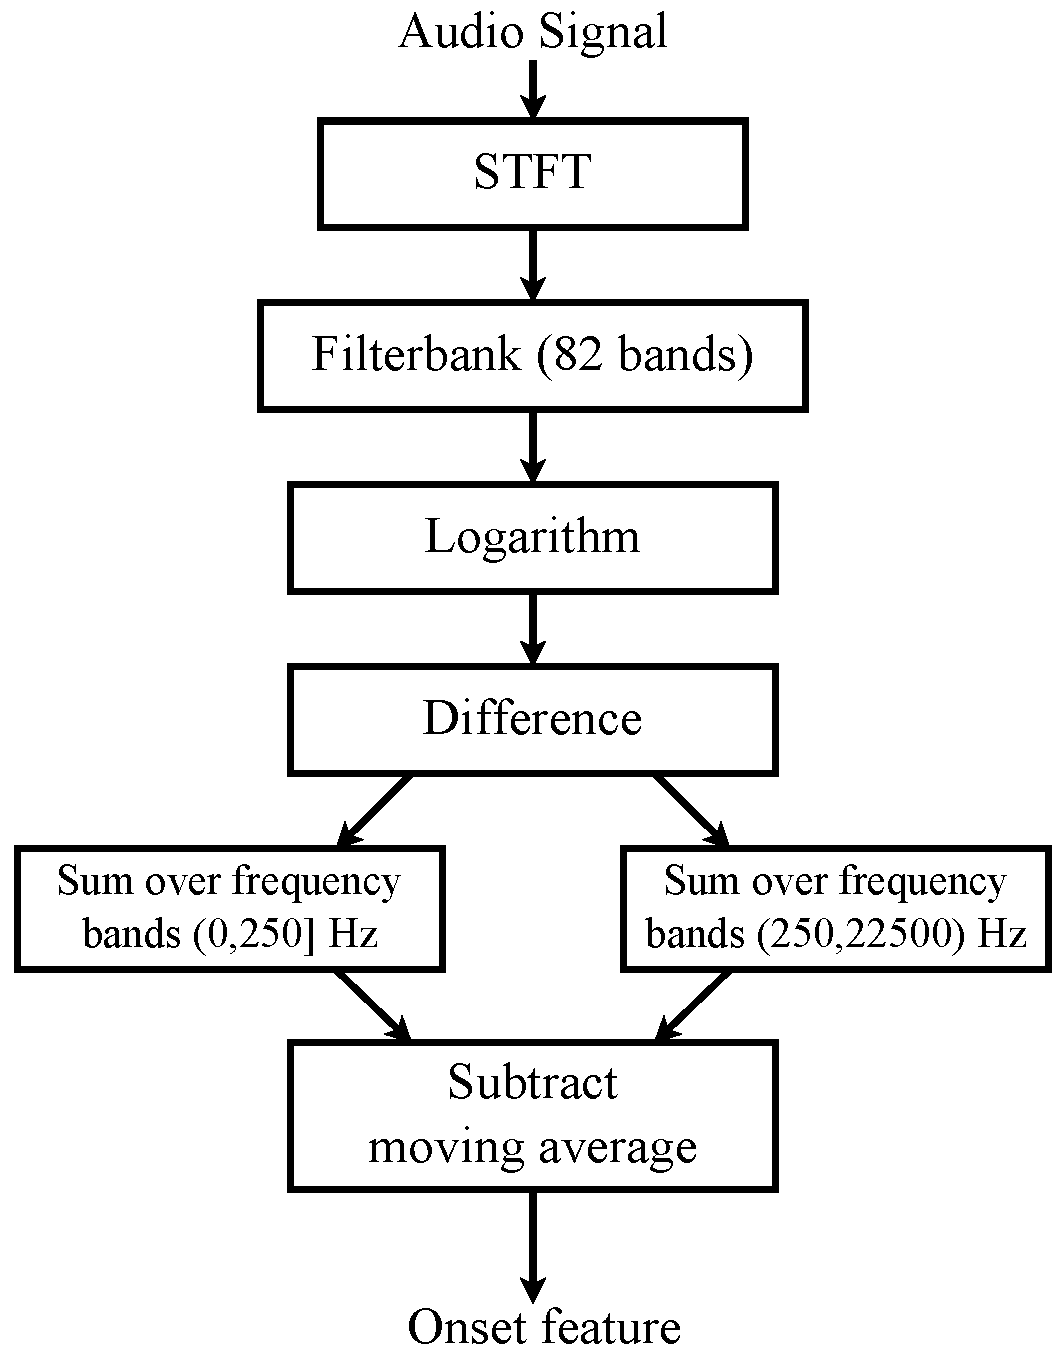
\includegraphics[scale=0.4]{blockDiags/obs-feat-computation.pdf}
	\caption[Computation of the spectral flux feature]{Computation of the spectral flux onset feature in two frequency bands, from \citeA{holzapfel:14:odd}.}
	\label{fig:obs:featcomp}
\end{figure}

The rhythm patterns are computed using a spectral flux\index{Spectral flux} feature (called LogFilt- SpecFlux as proposed by \citeA{bock:12:onseteval} and used further by \citeA{krebs:13:bpm}) that is used for detecting musical onsets in audio recordings. The \gls{STFT} of the audio signal with a window size of 46.4 ms (2047 samples of audio at a sampling rate of 44.1 kHz), DFT size of 2048 and hop size of 20 ms is computed from audio. The successive difference between frames of the logarithm of the filter bank energies in 82 different bands is then computed. Since the bass onsets have significant information about the rhythmic patterns, the features are computed in two frequency bands (Low: $\leq$ 250 Hz, High: $>$ 250 Hz) to additionally consider the bass onsets. The process of computing the spectral flux feature is outlined in \figref{fig:obs:featcomp}. 

Using beat and downbeat annotated training data, the audio features from all music pieces in a specific \gls{tala} are then grouped into cycle length sequences, and interpolated to equal lengths using a fine grid. A mean of all such cycle length sequence instances for a specific \gls{tala} is computed in both the frequency bands and used as a representative rhythmic pattern illustrated here. 

At the outset, it is necessary to note here that the patterns played in a \gls{tala} cycle are to be described using timing, energy and timbre descriptors. The rhythm patterns generated here using the spectral flux feature and can only explain timing and energy accents. A minor effect of timbre can be seen in these rhythm patterns, but are predominantly affected by the other two characteristics. These patterns are averaged over the whole dataset for a \gls{tala}, and hence cannot capture specific nuances of individual pieces, but only can give a broad perspective. The patterns here are indicative of the surface rhythm present in the audio recordings, and hence completely reflect the underlying canonical metrical structures. % List down other limitations of this approach. 

\figrefs{fig:tt:CMDf:adi}{fig:tt:CMD:khandaChapu}\ show the ensemble average of cycle length patterns over all the pieces in the dataset for each \gls{tala}, computed using the spectral flux feature in two different frequency bands as outlined above. In each figure, the bottom pane corresponds to the low frequency band ($\protect\obsLow$) and the top pane corresponds to the high frequency band ($\protect\obsHigh$). The abscissa is the beat number within the cycle (dotted lines), with 1 indicating the \gls{sama} (marked with a red line). The start of each \gls{anga} is indicated with beat numbers at the top of each pane (\gls{sama} shown as $\times$). The patterns in each figure pane is normalized so that maximum value is 1, to comment on relative onset strengths at different metrical positions of the cycle. 

The rhythm patterns are roughly indicative of the energies of mridangam strokes played in the cycle. In the figures, the bottom pane that shows the low frequency band has content from the left bass drum while the top pane has content predominantly from the right pitched drum (and additionally from the lead melody). Hence, for the purpose of this discussion, we use the terms left and right accents to refer to the accents in rhythm patterns shown on the bottom and top pane, respectively. The left and right accents provide interesting insights into the patterns played within a \gls{tala} cycle. In addition, these rhythm patterns help in meter tracking. 
% Tala pattern: CMDf-adi-all-lo230-superflux-mvavg-normZ, CMDf-adi-all-hi250-superflux-mvavg-normZ
\begin{figure}[t]
\captionsetup[subfigure]{labelformat=empty}
\centering
\subfloat[]{\label{fig:tt:CMDf:adi:hi}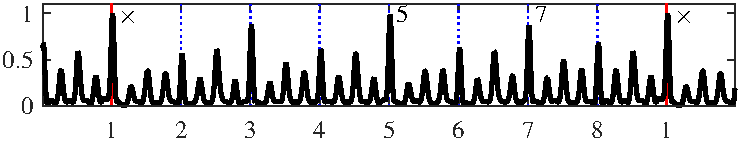
\includegraphics[width=\textwidth]{talaPatts/CMDf-adi-all-hi250-superflux-mvavg-normZ.pdf}} \\ \vspace{-1.35cm}
\subfloat[]{\label{fig:tt:CMDf:adi:lo}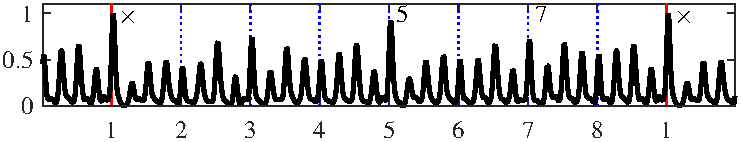
\includegraphics[width=\textwidth]{talaPatts/CMDf-adi-all-lo230-superflux-mvavg-normZ.pdf}}
\caption[Rhythm patterns in \gls{adi} \gls{tala} learned from \acrshort{CMDf} dataset]{Cycle length rhythmic patterns learned from \acrshort{CMDf} dataset for \gls{adi} \gls{tala}. In each of the following \protect\figrefs{fig:tt:CMDf:adi}{fig:tt:CMD:khandaChapu}, the patterns are computed from spectral flux feature and averaged over all the pieces in the dataset. The bottom/top pane corresponds to the low/high frequency bands, respectively. The abscissa is the beat number within the cycle (dotted lines), with 1 indicating the \gls{sama} (marked with a red line). The start of each \gls{anga} is indicated with beat numbers at the top of each pane (\gls{sama} shown as $\times$). The plot shows the cycle extended by a beat at the beginning and end to illustrate the cyclic nature of the \gls{tala}.}\label{fig:tt:CMDf:adi} %CMDf-adi-all-hi250-superflux-mvavg-normZ,CMDf-adi-all-lo230-superflux-mvavg-normZ
\end{figure}
%
% Tala pattern: CMD-adi-all-lo230-superflux-mvavg-normZ, CMD-adi-all-hi250-superflux-mvavg-normZ
\begin{figure}
\captionsetup[subfigure]{labelformat=empty}
\centering
\subfloat[]{\label{fig:tt:CMD:adi:hi}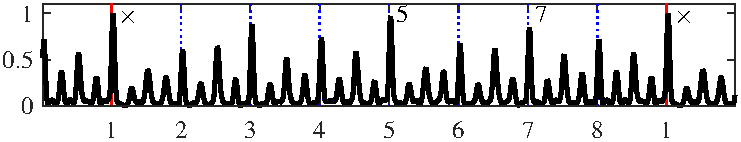
\includegraphics[width=\textwidth]{talaPatts/CMD-adi-all-hi250-superflux-mvavg-normZ.pdf}} \\ \vspace{-1.35cm}
\subfloat[]{\label{fig:tt:CMD:adi:lo}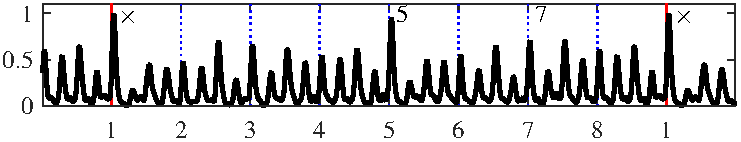
\includegraphics[width=\textwidth]{talaPatts/CMD-adi-all-lo230-superflux-mvavg-normZ.pdf}}
\caption[Rhythm patterns in \gls{adi} \gls{tala} learned from \acrshort{CMDs} dataset]{Cycle length rhythmic patterns learned from \acrshort{CMDs} dataset for \gls{adi} \gls{tala}.}\label{fig:tt:CMD:adi}
\end{figure}

We list down and discuss some salient qualitative observations from figures for each \gls{tala}, for both \acrshort{CMDf} dataset and its subset \acrshort{CMDs}. The \figrefs{fig:tt:CMDf:adi}{fig:tt:CMD:khandaChapu}\ show the cycle length rhythm patterns for all \glspl{tala} for both \acrshort{CMDf} and \acrshort{CMDs} datasets. For each \gls{tala}, we plot the rhythm patterns together to compare patterns across the short excerpts in \acrshort{CMDs} dataset and full length pieces in \acrshort{CMDf} dataset. 

Overall, we see stronger accents on the \glspl{akshara}, with \gls{sama} having the strongest accent in most cases. We can clearly see the accents organized in three different strengths, reflecting the metrical levels of the \gls{anga}, the beat and the \gls{akshara}. The two \gls{akshara} long beats in \gls{mishra chapu} and \gls{khanda chapu} \glspl{tala}, and the four \gls{akshara} long beats in \gls{adi} and \gls{rupaka} \glspl{tala} can be additionally seen. The patterns and \glspl{theka} played in Carnatic music are quite diverse, and no obvious representative \gls{tala} pattern can be inferred, apart from the varied accents at three metrical levels. 
% Tala pattern: CMDf-rupaka-all-lo230-superflux-mvavg-normZ, CMDf-rupaka-all-hi250-superflux-mvavg-normZ
\begin{figure}[t]
\captionsetup[subfigure]{labelformat=empty}
\centering
\subfloat[]{\label{fig:tt:CMDf:rupaka:hi}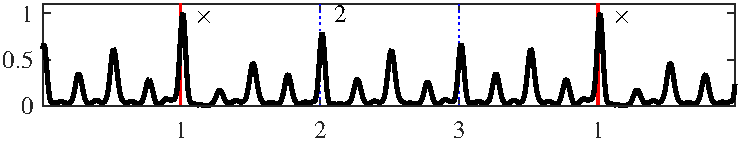
\includegraphics[width=\textwidth]{talaPatts/CMDf-rupaka-all-hi250-superflux-mvavg-normZ.pdf}} \\ \vspace{-1.35cm}
\subfloat[]{\label{fig:tt:CMDf:rupaka:lo}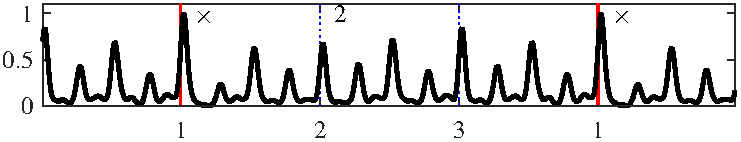
\includegraphics[width=\textwidth]{talaPatts/CMDf-rupaka-all-lo230-superflux-mvavg-normZ.pdf}}
\caption[Rhythm patterns in \gls{rupaka} \gls{tala} learned from \acrshort{CMDf} dataset]{Cycle length rhythmic patterns learned from \acrshort{CMDf} dataset for \gls{rupaka} \gls{tala}.}\label{fig:tt:CMDf:rupaka}
\end{figure}
%
% Tala pattern: CMD-rupaka-all-lo230-superflux-mvavg-normZ, CMD-rupaka-all-hi250-superflux-mvavg-normZ
\begin{figure}[t]
\captionsetup[subfigure]{labelformat=empty}
\centering
\subfloat[]{\label{fig:tt:CMD:rupaka:hi}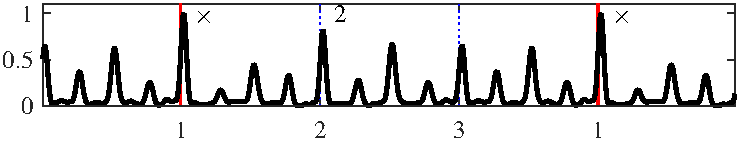
\includegraphics[width=\textwidth]{talaPatts/CMD-rupaka-all-hi250-superflux-mvavg-normZ.pdf}} \\ \vspace{-1.35cm}
\subfloat[]{\label{fig:tt:CMD:rupaka:lo}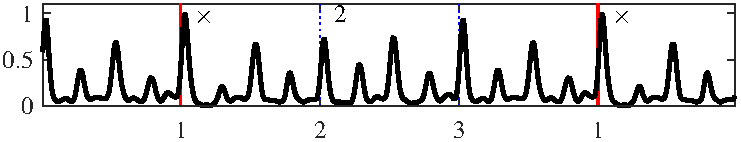
\includegraphics[width=\textwidth]{talaPatts/CMD-rupaka-all-lo230-superflux-mvavg-normZ.pdf}}
\caption[Rhythm patterns in \gls{rupaka} \gls{tala} learned from \acrshort{CMDs} dataset]{Cycle length rhythmic patterns learned from \acrshort{CMDs} dataset for \gls{rupaka} \gls{tala}.}\label{fig:tt:CMD:rupaka}
\end{figure}
%

The patterns illustrated here are average patterns that occur and do not tell us much about the various individual patterns that might occur in specific points in particular recordings. The \glspl{tala} are metrical structures that allow many different patterns to be played, and not a specific rhythm. It is further seen that the first \gls{akshara} after \gls{sama} has softer accents. Fewer strokes are played after the \gls{sama}, to emphasize that the \gls{sama} has just passed and a new cycle has begun. It might also perhaps indicate some form of recovery time after the intense stroke-playing towards the end of the cycle. 

The rhythm patterns computed using \acrshort{CMDs} dataset are very similar to those computed using \acrshort{CMDf} dataset, showing that \acrshort{CMDs} is a good representative subset of the larger \acrshort{CMDf}. Additionally, all the observations we make with patterns from \acrshort{CMDf} extend to \acrshort{CMDs}. We now discuss several \gls{tala} specific observations. 

The \figrefs{fig:tt:CMDf:adi}{fig:tt:CMD:adi}\ show the rhythm patterns for \gls{adi} \gls{tala}. We see that a three level hierarchy of \gls{anga}, beats and \glspl{akshara} is well demarcated. The \gls{akshara} at half cycle (beat 5) has an accent as strong as the \gls{sama}. The odd beats (marked 1, 3, 5, 7) have stronger right accents. The left accents are distributed through the cycle, with strong accents at half cycle.  
%
% Tala pattern: CMDf-mishraChapu-all-lo230-superflux-mvavg-normZ, CMDf-mishraChapu-all-hi250-superflux-mvavg-normZ
\begin{figure}[t]
\captionsetup[subfigure]{labelformat=empty}
\centering
\subfloat[]{\label{fig:tt:CMDf:mishraChapu:hi}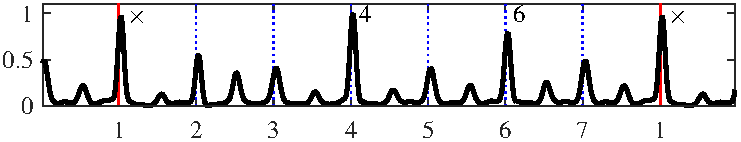
\includegraphics[width=\textwidth]{talaPatts/CMDf-mishraChapu-all-hi250-superflux-mvavg-normZ.pdf}} \\ \vspace{-1.35cm}
\subfloat[]{\label{fig:tt:CMDf:mishraChapu:lo}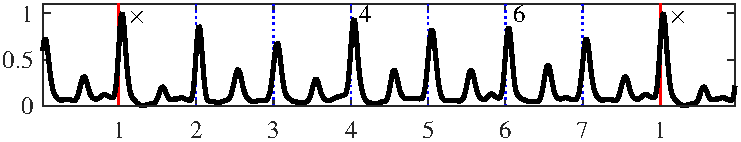
\includegraphics[width=\textwidth]{talaPatts/CMDf-mishraChapu-all-lo230-superflux-mvavg-normZ.pdf}}
\caption[Rhythm patterns in \gls{mishra chapu} \gls{tala} learned from \acrshort{CMDf} dataset]{Cycle length rhythmic patterns learned from \acrshort{CMDf} dataset for \gls{mishra chapu} \gls{tala}.}\label{fig:tt:CMDf:mishraChapu}
\end{figure}
%
%
% Tala pattern: CMD-mishraChapu-all-lo230-superflux-mvavg-normZ, CMD-mishraChapu-all-hi250-superflux-mvavg-normZ
\begin{figure}[t]
\captionsetup[subfigure]{labelformat=empty}
\centering
\subfloat[]{\label{fig:tt:CMD:mishraChapu:hi}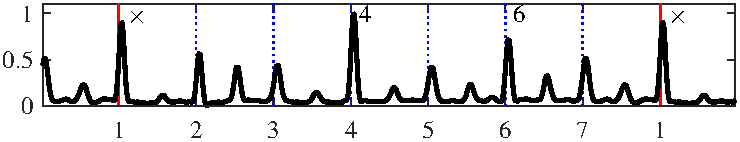
\includegraphics[width=\textwidth]{talaPatts/CMD-mishraChapu-all-hi250-superflux-mvavg-normZ.pdf}} \\ \vspace{-1.35cm}
\subfloat[]{\label{fig:tt:CMD:mishraChapu:lo}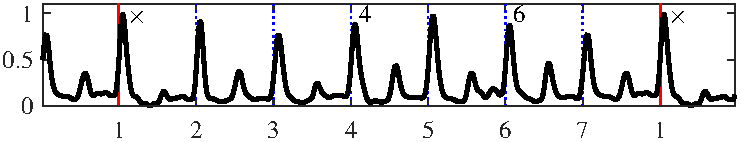
\includegraphics[width=\textwidth]{talaPatts/CMD-mishraChapu-all-lo230-superflux-mvavg-normZ.pdf}}
\caption[Rhythm patterns in \gls{mishra chapu} \gls{tala} learned from \acrshort{CMDs} dataset]{Cycle length rhythmic patterns learned from \acrshort{CMDs} dataset for \gls{mishra chapu} \gls{tala}.}\label{fig:tt:CMD:mishraChapu}
\end{figure}
%

The \figrefs{fig:tt:CMDf:rupaka}{fig:tt:CMD:rupaka}\ show the rhythm patterns for \gls{rupaka} \gls{tala}. Apart from the three level hierarachy of accents that is quite apparent, the half beat accent between the beats 2 and 3 are strong - indicating the often played 6+6 \gls{akshara} grouping structure of \gls{rupaka}, with a ternary meter.

The \figrefs{fig:tt:CMDf:mishraChapu}{fig:tt:CMD:mishraChapu}\ show the rhythm patterns for \gls{mishra chapu} \gls{tala}. We see that the \gls{anga} boundaries have strong left and right accents showing their use as anchor points to indicate the progression through the cycle. Though defined with a 3+2+2 \gls{akshara} grouping structure, a 1+2+2+2 structure is often seen in \gls{mishra chapu} \gls{tala}, which can be observed here, based on the strong left accent on beat 2. A additional strong left accent on beat 5 shows that it is also used as an anchor. 
%
% Tala pattern: CMDf-khandaChapu-all-lo230-superflux-mvavg-normZ, CMDf-khandaChapu-all-hi250-superflux-mvavg-normZ
\begin{figure}[t]
\captionsetup[subfigure]{labelformat=empty}
\centering
\subfloat[]{\label{fig:tt:CMDf:khandaChapu:hi}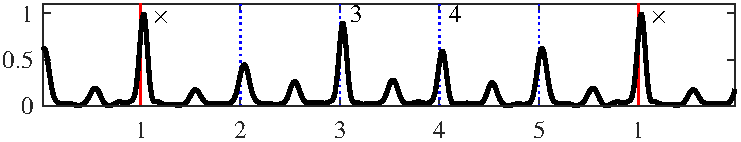
\includegraphics[width=\textwidth]{talaPatts/CMDf-khandaChapu-all-hi250-superflux-mvavg-normZ.pdf}} \\ \vspace{-1.35cm}
\subfloat[]{\label{fig:tt:CMDf:khandaChapu:lo}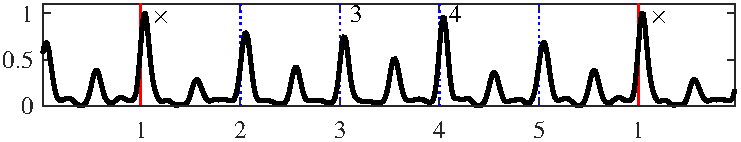
\includegraphics[width=\textwidth]{talaPatts/CMDf-khandaChapu-all-lo230-superflux-mvavg-normZ.pdf}}
\caption[Rhythm patterns in \gls{khanda chapu} \gls{tala} learned from \acrshort{CMDf} dataset]{Cycle length rhythmic patterns learned from \acrshort{CMDf} dataset for \gls{khanda chapu} \gls{tala}.}\label{fig:tt:CMDf:khandaChapu}
\end{figure}
%
%
% Tala pattern: CMD-khandaChapu-all-lo230-superflux-mvavg-normZ, CMD-khandaChapu-all-hi250-superflux-mvavg-normZ
\begin{figure}[t]
\captionsetup[subfigure]{labelformat=empty}
\centering
\subfloat[]{\label{fig:tt:CMD:khandaChapu:hi}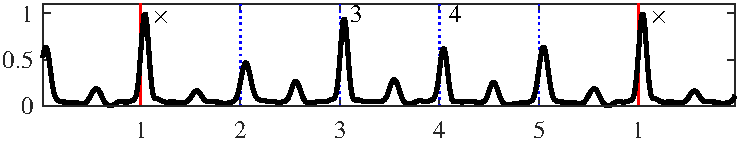
\includegraphics[width=\textwidth]{talaPatts/CMD-khandaChapu-all-hi250-superflux-mvavg-normZ.pdf}} \\ \vspace{-1.35cm}
\subfloat[]{\label{fig:tt:CMD:khandaChapu:lo}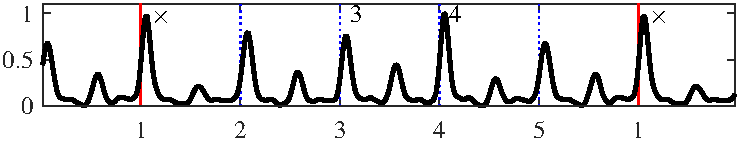
\includegraphics[width=\textwidth]{talaPatts/CMD-khandaChapu-all-lo230-superflux-mvavg-normZ.pdf}}
\caption[Rhythm patterns in \gls{khanda chapu} \gls{tala} learned from \acrshort{CMDs} dataset]{Cycle length rhythmic patterns learned from \acrshort{CMDs} dataset for \gls{khanda chapu} \gls{tala}.}\label{fig:tt:CMD:khandaChapu}
\end{figure}

The rhythm patterns of \gls{khanda chapu} \gls{tala} shown in \figrefs{fig:tt:CMDf:khandaChapu}{fig:tt:CMD:khandaChapu}\ have a strong left accent on beat 4, which is used an anchor within the cycle. A stronger right accent on beat 3 shows the progression through the unequal \glspl{anga}. The 2+1+2 \gls{akshara} grouping structure of \gls{khanda chapu} is often played out as 3+2 or 2+3, showing strong accents on beats 3 and 4. 

These are some observations from rhythm patterns that have interesting musicological significance. A professional Carnatic musician has informally validated these observations, but they still have to be formally studied in depth to make valid musicological conclusions. 
% An example of a corpus study with the dataset is an analysis of rhythmic patterns that occur in the dataset to see what musicological inferences can be made out of the analysis. We wish to independently verify 
% Statistical analysis of patterns in the dataset and what musicological inferences it can give out. 
%
%
%
% The bottom/top pane corresponds to the low/high frequency bands, respectively. The abscissa is the beat number within the cycle (dotted lines), with 1 indicating the \gls{sama} (marked with a red line). The start of each \gls{anga} is indicated with beat numbers at the top of each pane (\gls{sama} shown as $\times$).
\subsubsection{Applications of the Carnatic rhythm dataset}
The \acrshort{CMDf} dataset and its subset \acrshort{CMDs} dataset are intended to be test corpora for several automatic rhythm analysis tasks in Carnatic music. Possible tasks include \gls{sama} and beat tracking, tempo estimation and tracking, \gls{tala} recognition, rhythm based segmentation of musical audio, structural segmentation, audio to score/lyrics alignment, and rhythmic pattern analysis. In this thesis, these two datasets are primarily used for rhythmic pattern analysis and meter inference/tracking. Most of the research results are presented for \acrshort{CMDs} with some experiments extended to the full \acrshort{CMDf} dataset to verify their applicability to larger datasets.%\cite{ajay:14:rhythmJNMR, ajay:14:talaTrack} 
%
%
% Present stats about the dataset, then about distribution of ISI and IAI. Statistical analysis of patterns in the dataset and what musicological inferences it can give out. 
%
%% Dataset stats: CMD-IAI
\begin{figure}[ht]
%\captionsetup[subfigure]{labelformat=empty}
\begin{center}
\subfloat[\Gls{adi}]{\label{fig:dstats:CMD:IAI:adi}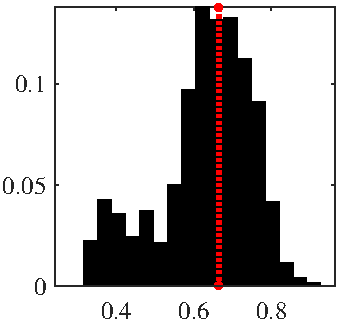
\includegraphics[scale=1]{dstats/CMD-adi-IAI.pdf}} \hspace{0.5cm} 
\subfloat[\Gls{rupaka}]{\label{fig:dstats:CMD:IAI:rupaka}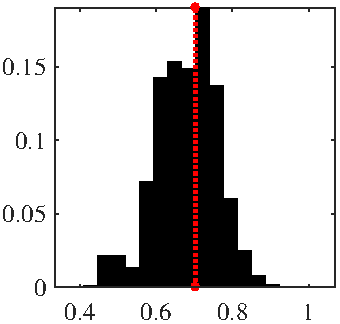
\includegraphics[scale=1]{dstats/CMD-rupaka-IAI.pdf}} \\ 
\subfloat[\Gls{mishra chapu}]{\label{fig:dstats:CMD:IAI:mishraChapu}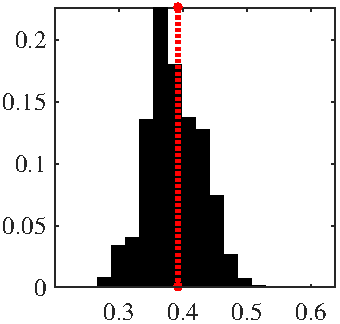
\includegraphics[scale=1]{dstats/CMD-mishraChapu-IAI.pdf}} \hspace{0.5cm} 
\subfloat[\Gls{khanda chapu}]{\label{fig:dstats:CMD:IAI:khandaChapu}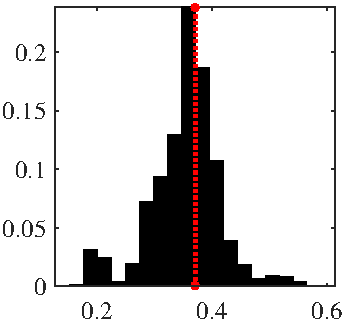
\includegraphics[scale=1]{dstats/CMD-khandaChapu-IAI.pdf}} \\ 
\caption[CMD-IAI]{CMD-IAI}\label{fig:dstats:CMD:IAI}
\end{center}
\end{figure}
%
%
% Dataset stats: CMD-IAInorm
\begin{figure}[ht]
%\captionsetup[subfigure]{labelformat=empty}
\begin{center}
\subfloat[\Gls{adi}]{\label{fig:dstats:CMD:IAInorm:adi}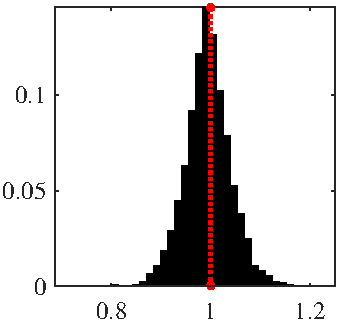
\includegraphics[scale=1]{dstats/CMD-adi-IAInorm.pdf}} \hspace{0.5cm} 
\subfloat[\Gls{rupaka}]{\label{fig:dstats:CMD:IAInorm:rupaka}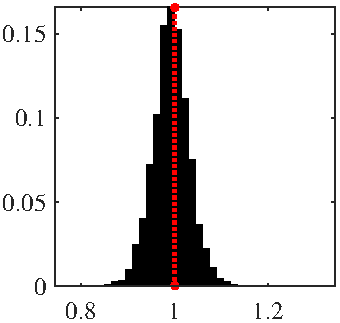
\includegraphics[scale=1]{dstats/CMD-rupaka-IAInorm.pdf}} \\ 
\subfloat[\Gls{mishra chapu}]{\label{fig:dstats:CMD:IAInorm:mishraChapu}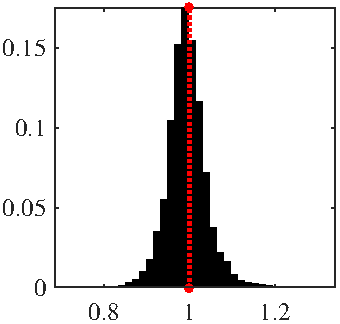
\includegraphics[scale=1]{dstats/CMD-mishraChapu-IAInorm.pdf}} \hspace{0.5cm} 
\subfloat[\Gls{khanda chapu}]{\label{fig:dstats:CMD:IAInorm:khandaChapu}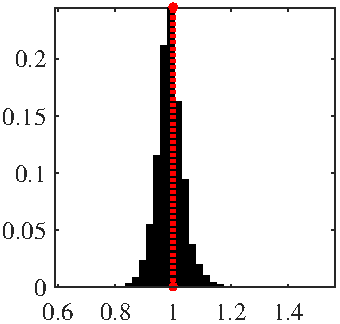
\includegraphics[scale=1]{dstats/CMD-khandaChapu-IAInorm.pdf}} \\ 
\caption[CMD-IAInorm]{CMD-IAInorm}\label{fig:dstats:CMD:IAInorm}
\end{center}
\end{figure}
%
%
% Dataset stats: CMD-ISI
\begin{figure}[ht]
%\captionsetup[subfigure]{labelformat=empty}
\begin{center}
\subfloat[\Gls{adi}]{\label{fig:dstats:CMD:ISI:adi}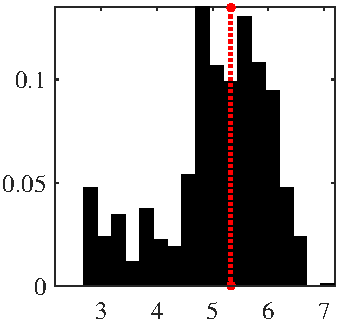
\includegraphics[scale=1]{dstats/CMD-adi-ISI.pdf}} \hspace{0.5cm} 
\subfloat[\Gls{rupaka}]{\label{fig:dstats:CMD:ISI:rupaka}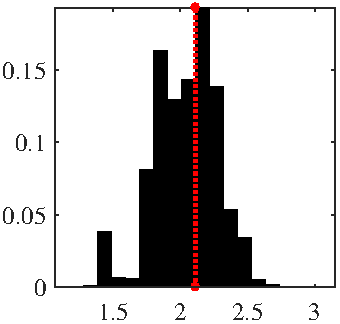
\includegraphics[scale=1]{dstats/CMD-rupaka-ISI.pdf}} \\ 
\subfloat[\Gls{mishra chapu}]{\label{fig:dstats:CMD:ISI:mishraChapu}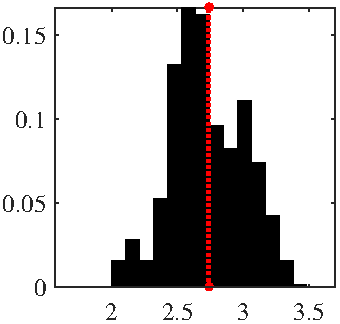
\includegraphics[scale=1]{dstats/CMD-mishraChapu-ISI.pdf}} \hspace{0.5cm} 
\subfloat[\Gls{khanda chapu}]{\label{fig:dstats:CMD:ISI:khandaChapu}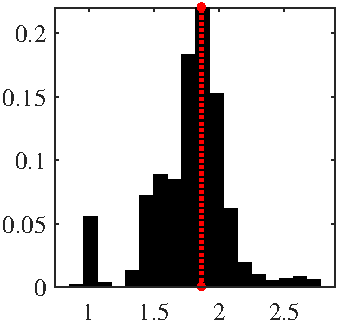
\includegraphics[scale=1]{dstats/CMD-khandaChapu-ISI.pdf}} \\ 
\caption[CMD-ISI]{CMD-ISI}\label{fig:dstats:CMD:ISI}
\end{center}
\end{figure}
%
%
% Dataset stats: CMD-ISInorm
\begin{figure}[ht]
%\captionsetup[subfigure]{labelformat=empty}
\begin{center}
\subfloat[\Gls{adi}]{\label{fig:dstats:CMD:ISInorm:adi}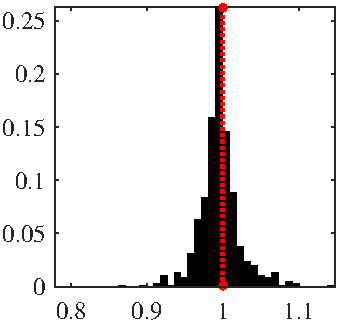
\includegraphics[scale=1]{dstats/CMD-adi-ISInorm.pdf}} \hspace{0.5cm} 
\subfloat[\Gls{rupaka}]{\label{fig:dstats:CMD:ISInorm:rupaka}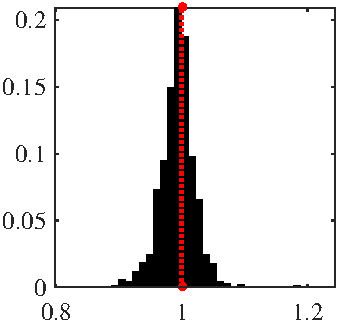
\includegraphics[scale=1]{dstats/CMD-rupaka-ISInorm.pdf}} \\ 
\subfloat[\Gls{mishra chapu}]{\label{fig:dstats:CMD:ISInorm:mishraChapu}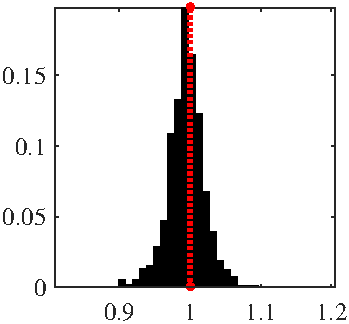
\includegraphics[scale=1]{dstats/CMD-mishraChapu-ISInorm.pdf}} \hspace{0.5cm} 
\subfloat[\Gls{khanda chapu}]{\label{fig:dstats:CMD:ISInorm:khandaChapu}\includegraphics[scale=1]{dstats/CMD-khandaChapu-ISInorm.pdf}} \\ 
\caption[CMD-ISInorm]{CMD-ISInorm}\label{fig:dstats:CMD:ISInorm}
\end{center}
\end{figure}
%\clearpage
%% Dataset stats: CMDf-IAI
\begin{figure}[ht]
%\captionsetup[subfigure]{labelformat=empty}
\begin{center}
\subfloat[\Gls{adi}]{\label{fig:dstats:CMDf:IAI:adi}\includegraphics[scale=1]{dstats/CMDf-adi-IAI.pdf}} \hspace{0.5cm} 
\subfloat[\Gls{rupaka}]{\label{fig:dstats:CMDf:IAI:rupaka}\includegraphics[scale=1]{dstats/CMDf-rupaka-IAI.pdf}} \\ 
\subfloat[\Gls{mishra chapu}]{\label{fig:dstats:CMDf:IAI:mishraChapu}\includegraphics[scale=1]{dstats/CMDf-mishraChapu-IAI.pdf}} \hspace{0.5cm} 
\subfloat[\Gls{khanda chapu}]{\label{fig:dstats:CMDf:IAI:khandaChapu}\includegraphics[scale=1]{dstats/CMDf-khandaChapu-IAI.pdf}} \\ 
\caption[CMDf-IAI]{CMDf-IAI}\label{fig:dstats:CMDf:IAI}
\end{center}
\end{figure}
%
%
% Dataset stats: CMDf-IAInorm
\begin{figure}[ht]
%\captionsetup[subfigure]{labelformat=empty}
\begin{center}
\subfloat[\Gls{adi}]{\label{fig:dstats:CMDf:IAInorm:adi}\includegraphics[scale=1]{dstats/CMDf-adi-IAInorm.pdf}} \hspace{0.5cm} 
\subfloat[\Gls{rupaka}]{\label{fig:dstats:CMDf:IAInorm:rupaka}\includegraphics[scale=1]{dstats/CMDf-rupaka-IAInorm.pdf}} \\ 
\subfloat[\Gls{mishra chapu}]{\label{fig:dstats:CMDf:IAInorm:mishraChapu}\includegraphics[scale=1]{dstats/CMDf-mishraChapu-IAInorm.pdf}} \hspace{0.5cm} 
\subfloat[\Gls{khanda chapu}]{\label{fig:dstats:CMDf:IAInorm:khandaChapu}\includegraphics[scale=1]{dstats/CMDf-khandaChapu-IAInorm.pdf}} \\ 
\caption[CMDf-IAInorm]{CMDf-IAInorm}\label{fig:dstats:CMDf:IAInorm}
\end{center}
\end{figure}
%
%
% Dataset stats: CMDf-ISI
\begin{figure}[ht]
%\captionsetup[subfigure]{labelformat=empty}
\begin{center}
\subfloat[\Gls{adi}]{\label{fig:dstats:CMDf:ISI:adi}\includegraphics[scale=1]{dstats/CMDf-adi-ISI.pdf}} \hspace{0.5cm} 
\subfloat[\Gls{rupaka}]{\label{fig:dstats:CMDf:ISI:rupaka}\includegraphics[scale=1]{dstats/CMDf-rupaka-ISI.pdf}} \\ 
\subfloat[\Gls{mishra chapu}]{\label{fig:dstats:CMDf:ISI:mishraChapu}\includegraphics[scale=1]{dstats/CMDf-mishraChapu-ISI.pdf}} \hspace{0.5cm} 
\subfloat[\Gls{khanda chapu}]{\label{fig:dstats:CMDf:ISI:khandaChapu}\includegraphics[scale=1]{dstats/CMDf-khandaChapu-ISI.pdf}} \\ 
\caption[CMDf-ISI]{CMDf-ISI}\label{fig:dstats:CMDf:ISI}
\end{center}
\end{figure}
%
%
% Dataset stats: CMDf-ISInorm
\begin{figure}[t]
%\captionsetup[subfigure]{labelformat=empty}
\begin{center}
\subfloat[\Gls{adi}]{\label{fig:dstats:CMDf:ISInorm:adi}\includegraphics[scale=1]{dstats/CMDf-adi-ISInorm.pdf}} \hspace{0.5cm} 
\subfloat[\Gls{rupaka}]{\label{fig:dstats:CMDf:ISInorm:rupaka}\includegraphics[scale=1]{dstats/CMDf-rupaka-ISInorm.pdf}} \\ 
\subfloat[\Gls{mishra chapu}]{\label{fig:dstats:CMDf:ISInorm:mishraChapu}\includegraphics[scale=1]{dstats/CMDf-mishraChapu-ISInorm.pdf}} \hspace{0.5cm} 
\subfloat[\Gls{khanda chapu}]{\label{fig:dstats:CMDf:ISInorm:khandaChapu}\includegraphics[scale=1]{dstats/CMDf-khandaChapu-ISInorm.pdf}} \\ 
\caption[CMDf-ISInorm]{CMDf-ISInorm}\label{fig:dstats:CMDf:ISInorm}
\end{center}
\end{figure}
%
%
%%%%%%%%%%%%%%%%%
%
\subsection{Hindustani music rhythm dataset}\label{sec:hmrdataset}
\acrfull{HMDf}\footnote{\url{http://compmusic.upf.edu/hindustani-rhythm-dataset}}\index{Hindustani music} is a rhythm annotated test corpus for automatic rhythm analysis tasks in Hindustani Music~\cite{ajay:16:spmodel}. The collection consists of audio excerpts from the CompMusic Hindustani research corpus, manually annotated time aligned markers indicating the progression through the \gls{taal} cycle, and the associated \gls{taal} related metadata. The dataset has pieces from four popular \glspl{taal} of Hindustani music (\tabref{tab:dataset:hmdf}), which encompasses a majority of Hindustani \gls{khayal} music. 

The audio recordings are chosen from the CompMusic Hindustani music research corpus. The pieces include a mix of vocal and instrumental recordings, new and old recordings, and span three \gls{lay} classes. For each taal, there are pieces in \gls{dhrut} (fast), \gls{madhyam} (medium) and \gls{vilambit} \gls{lay}. All pieces have \gls{tabla} as the percussion accompaniment. All the audio recordings in the dataset are 2 minute excerpts of full length pieces. Each piece is uniquely identified using the \gls{MBID} of the recording. The pieces are stereo, 160 kbps, mp3 files sampled at 44.1 kHz. The audio is also available as downmixed mono WAV files for experiments. 
%% HMDf table of dataset
\begin{table}[t]
\begin{center}
\begin{tabular}{@{}lrcrr@{}}
\toprule 
\Gls{taal} & \# Pieces & Total Duration & \# Ann. & \# Sam\tabularnewline
 &  & hours (min) &  & \tabularnewline
\midrule 
\Gls{teental} & 54 & 1.80 (108) & 17142 & 1081\tabularnewline
\Gls{ektal} & 58 & 1.93 (116) & 12999 & 1087\tabularnewline
\Gls{jhaptal} & 19 & 0.63 (38) & 3029 & 302\tabularnewline
\Gls{rupak} & 20 & 0.67 (40) & 2841 & 406\tabularnewline
\midrule 
Total & 151 & 5.03 (302) & 36011 & 2876\tabularnewline
\bottomrule 
\end{tabular}
\end{center}
\protect\caption[\acrshort{HMDf} dataset description]{\acrshort{HMDf} dataset showing the total duration and number of annotations. \#Sam shows the number of \gls{sam} annotations and \#Ann. shows the number of \gls{matra} annotations (including \glspl{sam}).}
\label{tab:dataset:hmdf}
\end{table}
%% HMDf table of datastats
\begin{table}[t]
\begin{center}
\begin{tabular}{@{}lccc@{}}
\toprule 
\Gls{taal} & $\overline{\isi} \pm \sigma_s$ & $\overline{\ibi} \pm \sigma_b$  & $[{\isi}_{,\min} \, , \,  {\isi}_{,\max} ]$ \tabularnewline
\midrule 
\Gls{teental} & 10.36 $\pm$ 9.875 & 0.65 $\pm$ 0.617 & {[}2.32, 44.14{]}\tabularnewline
\Gls{ektal} & 30.20 $\pm$ 26.258 & 2.52 $\pm$ 2.188 & {[}2.23, 69.73{]}\tabularnewline
\Gls{jhaptal} & 8.51 $\pm$ 3.149 & 0.85 $\pm$ 0.315 & {[}4.06, 16.23{]}\tabularnewline
\Gls{rupak} & 7.11 $\pm$ 3.360 & 1.02 $\pm$ 0.480 & {[}2.82, 16.09{]}\tabularnewline
\bottomrule 
\end{tabular}
\end{center}
\protect\caption[\Gls{taal} cycle length indicators for \acrshort{HMDf} dataset]{\Gls{taal} cycle length indicators for \acrshort{HMDf} dataset. $\overline{\isi}$ and $\sigma_s$ indicate the mean and standard deviation of the median inter-\gls{sam} interval of the pieces, respectively. $\overline{\ibi}$ and $\sigma_b$ indicate the mean and standard deviation of the median inter-\gls{matra} interval of the pieces, respectively. $[{\isi}_{,\min} \, , \,  {\isi}_{,\max}]$ indicate the minimum and maximum value of $\isi$ and hence the range of $\isi$ in the dataset. All values in the table are in seconds.}
\label{tab:datastat:hmdf}
\end{table}
%% HMDl table of dataset
\begin{table}[t]
\begin{center}
\begin{tabular}{@{}lrcrr@{}}
\toprule 
\Gls{taal} & \# Pieces & Total Duration & \# Ann. & \# Sam\tabularnewline
 &  & hours (min) &  & \tabularnewline
\midrule 
\Gls{teental} & 13 & 0.43 (26) & 1020 & 65\tabularnewline
\Gls{ektal} & 32 & 1.07 (64) & 967 & 79\tabularnewline
\Gls{jhaptal} & 6 & 0.2 (12) & 592 & 59\tabularnewline
\Gls{rupak} & 8 & 0.27 (16) & 701 & 101\tabularnewline
\midrule 
Total & 59 & 1.97 (118) & 3280 & 304\tabularnewline
\bottomrule 
\end{tabular}
\end{center}
\protect\caption[\acrshort{HMDl} dataset description]{\acrshort{HMDl} dataset showing the total duration and number of annotations. \#Sam shows the number of \gls{sam} annotations and \#Ann. shows the number of \gls{matra} annotations (including \glspl{sam}).}
\label{tab:dataset:hmdl}
\end{table}
%% HMDl table of datastats
\begin{table}[t]
\begin{center}
\begin{tabular}{@{}lccc@{}}
\toprule 
\Gls{taal} & $\overline{\isi} \pm \sigma_s$ & $\overline{\ibi} \pm \sigma_b$  & $[{\isi}_{,\min} \, , \,  {\isi}_{,\max} ]$ \tabularnewline
\midrule 
\Gls{teental} & 26.16 $\pm$ 7.963  & 1.63 $\pm$ 0.498 & {[}18.57, 44.14{]}\tabularnewline
\Gls{ektal} & 52.16 $\pm$ 12.531 & 4.35 $\pm$ 1.044 & {[}14.43, 69.73{]}\tabularnewline
\Gls{jhaptal} & 12.30 $\pm$ 1.935 & 1.23 $\pm$ 0.194 & {[}10.20, 16.23{]}\tabularnewline
\Gls{rupak} & 10.28 $\pm$ 3.050 & 1.47 $\pm$ 0.436 & {[}6.95, 16.09{]}\tabularnewline
\bottomrule 
\end{tabular}
\end{center}
\protect\caption[\Gls{taal} cycle length indicators for \acrshort{HMDl} dataset]{\Gls{taal} cycle length indicators for \acrshort{HMDl} dataset. $\overline{\isi}$ and $\sigma_s$ indicate the mean and standard deviation of the median inter-\gls{sam} interval of the pieces, respectively. $\overline{\ibi}$ and $\sigma_b$ indicate the mean and standard deviation of the median inter-\gls{matra} interval of the pieces, respectively. $[{\isi}_{,\min} \, , \,  {\isi}_{,\max}]$ indicate the minimum and maximum value of $\isi$ and hence the range of $\isi$ in the dataset. All values in the table are in seconds.}
\label{tab:datastat:hmdl}
\end{table}
%% HMDs table of dataset
\begin{table}[t]
\begin{center}
\begin{tabular}{@{}lrcrr@{}}
\toprule 
\Gls{taal} & \# Pieces & Total Duration & \# Ann. & \# Sam\tabularnewline
 &  & hours (min) &  & \tabularnewline
\midrule 
\Gls{teental} & 41 & 1.37 (82) & 16122 & 1016\tabularnewline
\Gls{ektal} & 26 & 0.87 (52) & 12032 & 1008\tabularnewline
\Gls{jhaptal} & 13 & 0.43 (26) & 2437 & 243\tabularnewline
\Gls{rupak} & 12 & 0.40 (24) & 2140 & 305\tabularnewline
\midrule 
Total & 92 & 3.07 (184) & 32731 & 2572\tabularnewline
\bottomrule 
\end{tabular}
\end{center}
\protect\caption[\acrshort{HMDs} dataset description]{\acrshort{HMDs} dataset showing the total duration and number of annotations. \#Sam shows the number of \gls{sam} annotations and \#Ann. shows the number of \gls{matra} annotations (including \glspl{sam}).}
\label{tab:dataset:hmds}
\end{table}
%% HMDs table of datastats
\begin{table}[t]
\begin{center}
\begin{tabular}{@{}lccc@{}}
\toprule 
\Gls{taal} & $\overline{\isi} \pm \sigma_s$ & $\overline{\ibi} \pm \sigma_b$  & $[{\isi}_{,\min} \, , \,  {\isi}_{,\max} ]$ \tabularnewline
\midrule 
\Gls{teental} & 5.35 $\pm$ 1.823 & 0.33 $\pm$ 0.114 & {[}2.32, 9.89{]}\tabularnewline
\Gls{ektal} & 3.17 $\pm$ 0.471 & 0.26 $\pm$ 0.039 & {[}2.23, 4.11{]}\tabularnewline
\Gls{jhaptal} & 6.77 $\pm$ 1.688 & 0.68 $\pm$ 0.169 & {[}4.06, 9.97{]}\tabularnewline
\Gls{rupak} & 5.00 $\pm$ 1.191 & 0.71 $\pm$ 0.170 & {[}2.82, 6.68{]}\tabularnewline
\bottomrule 
\end{tabular}
\end{center}
\protect\caption[\Gls{taal} cycle length indicators for \acrshort{HMDs} dataset]{\Gls{taal} cycle length indicators for \acrshort{HMDs} dataset. $\overline{\isi}$ and $\sigma_s$ indicate the mean and standard deviation of the median inter-\gls{sam} interval of the pieces, respectively. $\overline{\ibi}$ and $\sigma_b$ indicate the mean and standard deviation of the median inter-\gls{matra} interval of the pieces, respectively. $[{\isi}_{,\min} \, , \,  {\isi}_{,\max}]$ indicate the minimum and maximum value of $\isi$ and hence the range of $\isi$ in the dataset. All values in the table are in seconds.}
\label{tab:datastat:hmds}
\end{table}
% Dataset stats: HMDl-ISI
\begin{figure}[t]
%\captionsetup[subfigure]{labelformat=empty}
\centering
\subfloat[\Gls{teental}]{\label{fig:dstats:HMDl:ISI:teen}\includegraphics[scale=0.9]{dstats/HMDl-teen-ISI.pdf}} \hspace{0.5cm} 
\subfloat[\Gls{ektal}]{\label{fig:dstats:HMDl:ISI:ek}\includegraphics[scale=0.9]{dstats/HMDl-ek-ISI.pdf}} \\ 
\subfloat[\Gls{jhaptal}]{\label{fig:dstats:HMDl:ISI:jhap}\includegraphics[scale=0.9]{dstats/HMDl-jhap-ISI.pdf}} \hspace{0.5cm} 
\subfloat[\Gls{rupak}]{\label{fig:dstats:HMDl:ISI:rupak}\includegraphics[scale=0.9]{dstats/HMDl-rupak-ISI.pdf}} \\ 
\caption[Histogram of $\protect\isi$ in the \acrshort{HMDl} dataset]{A histogram of the inter-\gls{sam} interval $\protect\isi$ in the \acrshort{HMDl} dataset for each \gls{taal}. The ordinate is the fraction of the total count corresponding to the $\ibi$ value shown in abscissa. The median $\isi$ for each \gls{taal} is shown as a red dotted line.}\label{fig:dstats:HMDl:ISI}
\end{figure}
%
% Dataset stats: HMDl-IAI
\begin{figure}[t]
%\captionsetup[subfigure]{labelformat=empty}
\centering
\subfloat[\Gls{teental}]{\label{fig:dstats:HMDl:IAI:teen}\includegraphics[scale=0.9]{dstats/HMDl-teen-IAI.pdf}} \hspace{0.5cm} 
\subfloat[\Gls{ektal}]{\label{fig:dstats:HMDl:IAI:ek}\includegraphics[scale=0.9]{dstats/HMDl-ek-IAI.pdf}} \\ 
\subfloat[\Gls{jhaptal}]{\label{fig:dstats:HMDl:IAI:jhap}\includegraphics[scale=0.9]{dstats/HMDl-jhap-IAI.pdf}} \hspace{0.5cm} 
\subfloat[\Gls{rupak}]{\label{fig:dstats:HMDl:IAI:rupak}\includegraphics[scale=0.9]{dstats/HMDl-rupak-IAI.pdf}} \\ 
\caption[Histogram of $\protect\ibi$ in the \acrshort{HMDl} dataset]{A histogram of the inter-\gls{matra} interval $\protect\ibi$ in the \acrshort{HMDl} dataset for each \gls{taal}. The ordinate is the fraction of the total count corresponding to the $\ibi$ value shown in abscissa. The median $\ibi$ for each \gls{taal} is shown as a red dotted line.}\label{fig:dstats:HMDl:IAI}
\end{figure}
%
% Dataset stats: HMDs-ISI
\begin{figure}[t]
%\captionsetup[subfigure]{labelformat=empty}
\centering
\subfloat[\Gls{teental}]{\label{fig:dstats:HMDs:ISI:teen}\includegraphics[scale=0.9]{dstats/HMDs-teen-ISI.pdf}} \hspace{0.5cm} 
\subfloat[\Gls{ektal}]{\label{fig:dstats:HMDs:ISI:ek}\includegraphics[scale=0.9]{dstats/HMDs-ek-ISI.pdf}} \\ 
\subfloat[\Gls{jhaptal}]{\label{fig:dstats:HMDs:ISI:jhap}\includegraphics[scale=0.9]{dstats/HMDs-jhap-ISI.pdf}} \hspace{0.5cm} 
\subfloat[\Gls{rupak}]{\label{fig:dstats:HMDs:ISI:rupak}\includegraphics[scale=0.9]{dstats/HMDs-rupak-ISI.pdf}} \\ 
\caption[Histogram of $\protect\isi$ in the \acrshort{HMDs} dataset]{A histogram of the inter-\gls{sam} interval $\protect\isi$ in the \acrshort{HMDs} dataset for each \gls{taal}. The ordinate is the fraction of the total count corresponding to the $\ibi$ value shown in abscissa. The median $\isi$ for each \gls{taal} is shown as a red dotted line.}\label{fig:dstats:HMDs:ISI}
\end{figure}
%
% Dataset stats: HMDs-IAI
\begin{figure}[t]
%\captionsetup[subfigure]{labelformat=empty}
\centering
\subfloat[\Gls{teental}]{\label{fig:dstats:HMDs:IAI:teen}\includegraphics[scale=0.9]{dstats/HMDs-teen-IAI.pdf}} \hspace{0.5cm} 
\subfloat[\Gls{ektal}]{\label{fig:dstats:HMDs:IAI:ek}\includegraphics[scale=0.9]{dstats/HMDs-ek-IAI.pdf}} \\ 
\subfloat[\Gls{jhaptal}]{\label{fig:dstats:HMDs:IAI:jhap}\includegraphics[scale=0.9]{dstats/HMDs-jhap-IAI.pdf}} \hspace{0.5cm} 
\subfloat[\Gls{rupak}]{\label{fig:dstats:HMDs:IAI:rupak}\includegraphics[scale=0.9]{dstats/HMDs-rupak-IAI.pdf}} \\ 
\caption[Histogram of $\protect\ibi$ in the \acrshort{HMDs} dataset]{A histogram of the inter-\gls{matra} interval $\protect\ibi$ in the \acrshort{HMDs} dataset for each \gls{taal}. The ordinate is the fraction of the total count corresponding to the $\ibi$ value shown in abscissa. The median $\ibi$ for each \gls{taal} is shown as a red dotted line.}\label{fig:dstats:HMDs:IAI}
\end{figure}
%
% Dataset stats: HMDl-ISInorm
\begin{figure}[t]
%\captionsetup[subfigure]{labelformat=empty}
\centering
\subfloat[\Gls{teental}]{\label{fig:dstats:HMDl:ISInorm:teen}\includegraphics[scale=0.9]{dstats/HMDl-teen-ISInorm.pdf}} \hspace{0.5cm} 
\subfloat[\Gls{ektal}]{\label{fig:dstats:HMDl:ISInorm:ek}\includegraphics[scale=0.9]{dstats/HMDl-ek-ISInorm.pdf}} \\ 
\subfloat[\Gls{jhaptal}]{\label{fig:dstats:HMDl:ISInorm:jhap}\includegraphics[scale=0.9]{dstats/HMDl-jhap-ISInorm.pdf}} \hspace{0.5cm} 
\subfloat[\Gls{rupak}]{\label{fig:dstats:HMDl:ISInorm:rupak}\includegraphics[scale=0.9]{dstats/HMDl-rupak-ISInorm.pdf}} \\ 
\caption[Histogram of median normalized $\protect\isi$ in the \acrshort{HMDl} dataset]{A histogram of the median normalized inter-\gls{sam} interval $\protect\isi$ in the \acrshort{HMDl} dataset for each \gls{taal}. The ordinate is the fraction of the total count corresponding to the normalized $\isi$ value shown in abscissa.}\label{fig:dstats:HMDl:ISInorm}
\end{figure}
%
% Dataset stats: HMDl-IAInorm
\begin{figure}[t]
%\captionsetup[subfigure]{labelformat=empty}
\centering
\subfloat[\Gls{teental}]{\label{fig:dstats:HMDl:IAInorm:teen}\includegraphics[scale=0.9]{dstats/HMDl-teen-IAInorm.pdf}} \hspace{0.5cm} 
\subfloat[\Gls{ektal}]{\label{fig:dstats:HMDl:IAInorm:ek}\includegraphics[scale=0.9]{dstats/HMDl-ek-IAInorm.pdf}} \\ 
\subfloat[\Gls{jhaptal}]{\label{fig:dstats:HMDl:IAInorm:jhap}\includegraphics[scale=0.9]{dstats/HMDl-jhap-IAInorm.pdf}} \hspace{0.4cm} 
\subfloat[\Gls{rupak}]{\label{fig:dstats:HMDl:IAInorm:rupak}\includegraphics[scale=0.9]{dstats/HMDl-rupak-IAInorm.pdf}} \\ 
\caption[Histogram of median normalized $\protect\ibi$ in the \acrshort{HMDl} dataset]{A histogram of the median normalized inter-\gls{matra} interval $\protect\ibi$ in the \acrshort{HMDl} dataset for each \gls{taal}. The ordinate is the fraction of the total count corresponding to the normalized $\ibi$ value shown in abscissa.}\label{fig:dstats:HMDl:IAInorm}
\centering
\end{figure}
%

There are several annotations that accompany each audio file in the dataset. The primary annotations are audio synchronized time-stamps indicating the different metrical positions in the \gls{taal} cycle. The \gls{sam} and \glspl{matra} of the cycle are annotated. The annotations were created using Sonic Visualizer by tapping to music and manually correcting the taps. Each annotation has a time-stamp and an associated numeric label that indicates the \gls{matra} position in the \gls{taal} cycle illustrated in \figref{fig:taal:hindustani}. The \glspl{sam} are indicated using the numeral 1. The time varying tempo of the piece can be obtained from the \gls{matra} and \gls{sam} annotations. 

For each excerpt, the \gls{taal} and the \gls{lay} of the piece are recorded. Each excerpt can be uniquely identified and located with the \gls{MBID} of the recording, and the relative start and end times of the excerpt within the whole recording. The artist, release, the lead instrument, and the \gls{raag} of the piece are additional editorial metadata obtained from the release. There are optional comments on audio quality and annotation specifics. The annotations and the associated metadata have been verified for correctness and completeness by a professional Hindustani musician and musicologist. 

The \acrshort{HMDf} dataset is described in \tabref{tab:dataset:hmdf}, showing the four \glspl{taal} and the number of pieces for each \gls{taal}, totaling to 151 pieces. The total duration of audio in the dataset is about 5 hours, with 36011 time-aligned \gls{matra} annotations of which 2876 are \gls{sam} annotations. \tabref{tab:datastat:hmdf} shows a basic statistical analysis of the \gls{taal} cycle length indicators in the dataset to understand the tempo characteristics and the range of the metrical cycle lengths in the dataset. The large range of tempi seen in Hindustani music is reflected in the dataset, with the values of median inter-\gls{sam} interval $\overline{\isi}$, \gls{ektal} cycle lengths ranging from 2.2 seconds to 69.7 seconds, which is about 5 tempo octaves. This also shows that the \gls{matra} period can vary from less than 150 ms to over 6 seconds. This huge range of cycle lengths and \gls{matra} periods is a significant challenge in automatic meter analysis of Hindustani music. Across different \glspl{taal}, we see that \gls{teental} and \gls{ektal} have the largest range of $\overline{\isi}$, since they are performed in all the \gls{lay} classes, \gls{vilambit} to \gls{dhrut}. \Gls{jhaptal} and \gls{rupak} have smaller $\overline{\isi}$ ranges. 

The dataset consists of excerpts with a wide tempo range from 10 \mpm\ (\glspl{matra} per minute) to 370 \mpm. As discussed in \chapref{chap:bkgnd}, Hindustani music divides tempo into three main tempo classes (\gls{lay}). Since no exact tempo ranges are defined for these classes, we determined suitable values, measured in \glspl{matra} per minute (\mpm), in correspondence with a professional Hindustani musician as 10-60 \mpm, 60-150 \mpm, and $>$150 \mpm\ for the slow (\gls{vilambit}), medium (\gls{madhyam}), and fast (\gls{dhrut}) tempi, respectively. 

The \gls{lay} of a piece has a significant effect on meter tracking and rhythm analysis due to this wide range of possible tempo. To study any effects of the tempo class, the full \acrshort{HMDf} dataset is divided into two other subsets - the long cycle duration subset called the \acrshort{HMDl} dataset (shown in \tabref{tab:dataset:hmdl}) consisting of \gls{vilambit} pieces with a median tempo between 10-60 \mpm, and the short cycle duration subset \acrshort{HMDs} dataset (shown in \tabref{tab:dataset:hmds}) with \gls{madhyam} \gls{lay} (60-150 \mpm) and the \gls{dhrut} \gls{lay} (150+ \mpm) pieces. 

\acrshort{HMDl} dataset shown in \tabref{tab:dataset:hmdl} consists of 59 pieces in \gls{vilambit} \gls{lay}, with over 3200 \gls{matra} and \gls{sam} annotations. A majority of pieces are in \gls{ektal} and \gls{teental}. Since its very uncommon for a piece to be performed in \gls{vilambit} \gls{lay} \gls{jhaptal} and \gls{rupak}, there are only 6 and 8 pieces for those \glspl{taal}, respectively. As described with \acrshort{HMDf}, a basic statistical analysis of the \gls{taal} cycle length indicators in \tabref{tab:datastat:hmdl} shows that the median inter-\gls{sam} interval and its range for \gls{jhaptal} and \gls{rupak} are less than that for \gls{teental} and \gls{ektal}.

\acrshort{HMDs} dataset in \tabref{tab:dataset:hmds} consists on 92 pieces in \gls{madhyam} and \gls{dhrut} \gls{lay}, with over 3 hours of audio and over 32700 \gls{matra} and \gls{sam} annotations. A basic statistical analysis of the \gls{taal} cycle length indicators in \tabref{tab:datastat:hmds} shows that the pieces of \gls{teental} and \gls{ektal} have higher tempi in the dataset. Comparing the median \gls{matra} period for \gls{ektal} between \tabref{tab:datastat:hmdl} (4.35 second) and \tabref{tab:datastat:hmds} (0.26 second) shows that \gls{ektal} is performed either in \gls{vilambit} or \gls{dhrut} and its rare for a piece to be performed in \gls{madhyam} \gls{lay} \gls{ektal}.

The pieces is Hindustani music have a tempo class indicated but not a specific tempo value, nor are they performed to a metronome. The tempo varies over a piece in time - often the tempo increases with time. Hence, in addition to the median values tabulated in \tabref{tab:datastat:hmdf} we present further analysis of the inter-\gls{sam} interval (\isi) and inter-\gls{matra} interval (\ibi) for each \gls{taal}. For better comparison, we present this analysis for each data subset \acrshort{HMDl} and \acrshort{HMDs} separately. 

A histogram of $\isi$ and $\ibi$ for each \gls{taal} for \acrshort{HMDl} dataset is shown in \figref{fig:dstats:HMDl:ISI} and \figref{fig:dstats:HMDl:IAI}, respectively, and those for \acrshort{HMDs} dataset is shown in \figref{fig:dstats:HMDs:ISI} and \figref{fig:dstats:HMDs:IAI}, respectively. These figures show the distribution of cycle lengths in the dataset over the whole range of $\isi$ for each \gls{taal}, around the median value. The large range of $\isi$ and $\ibi$ values and an irregular distribution spanning the whole range is seen with both datasets, unlike the Carnatic music \acrshort{CMDf} dataset with a smaller tightly defined range of tempo. 

In addition, similar to what was presented for Carnatic music, to illustrate and measure the time varying tempo of music pieces in Hindustani music, we normalize all the $\isi$ and $\ibi$ values in a piece by the median in the piece to obtain median normalized $\isi$ and $\ibi$ values, a histogram of which is shown in \figref{fig:dstats:HMDl:ISInorm} and \figref{fig:dstats:HMDl:IAInorm}, respectively for \acrshort{HMDl} dataset and \figref{fig:dstats:HMDs:ISInorm} and \figref{fig:dstats:HMDs:IAInorm}, respectively for \acrshort{HMDs} dataset. These histograms are centered around 1 and normalized by the median. 

From the figures, it is clear that the tempo is time varying but with less than about 10\% maximum deviation from the median tempo of the piece for all \glspl{taal}. This is in contrast to Carnatic music where the median normalized tempo had a higher maximum deviation ($\sim$ 20 \%). One possible reason for this lower tempo deviation in Hindustani music compared to Carnatic music is because of less rhythmic improvisation, with the tabla acting as an accurate timekeeper. However, this could also be possibly due to the fact that the Hindustani pieces in the dataset are two minute short excerpts, compared to full length Carnatic pieces in the \acrshort{CMDf} dataset, and hence have lower tempo variability. 
%% Dataset stats: HMDl-IAI
\begin{figure}[t]
%\captionsetup[subfigure]{labelformat=empty}
\centering
\subfloat[\Gls{teental}]{\label{fig:dstats:HMDl:IAI:teen}\includegraphics[scale=1]{dstats/HMDl-teen-IAI.pdf}} \hspace{0.5cm} 
\subfloat[\Gls{ektal}]{\label{fig:dstats:HMDl:IAI:ek}\includegraphics[scale=1]{dstats/HMDl-ek-IAI.pdf}} \\ 
\subfloat[\Gls{jhaptal}]{\label{fig:dstats:HMDl:IAI:jhap}\includegraphics[scale=1]{dstats/HMDl-jhap-IAI.pdf}} \hspace{0.5cm} 
\subfloat[\Gls{rupak}]{\label{fig:dstats:HMDl:IAI:rupak}\includegraphics[scale=1]{dstats/HMDl-rupak-IAI.pdf}} \\ 
\caption[HMDl-IAI]{HMDl-IAI}\label{fig:dstats:HMDl:IAI}
\end{figure}
%
%
% Dataset stats: HMDl-IAInorm
\begin{figure}[t]
%\captionsetup[subfigure]{labelformat=empty}
\centering
\subfloat[\Gls{teental}]{\label{fig:dstats:HMDl:IAInorm:teen}\includegraphics[scale=1]{dstats/HMDl-teen-IAInorm.pdf}} \hspace{0.5cm} 
\subfloat[\Gls{ektal}]{\label{fig:dstats:HMDl:IAInorm:ek}\includegraphics[scale=1]{dstats/HMDl-ek-IAInorm.pdf}} \\ 
\subfloat[\Gls{jhaptal}]{\label{fig:dstats:HMDl:IAInorm:jhap}\includegraphics[scale=1]{dstats/HMDl-jhap-IAInorm.pdf}} \hspace{0.5cm} 
\subfloat[\Gls{rupak}]{\label{fig:dstats:HMDl:IAInorm:rupak}\includegraphics[scale=1]{dstats/HMDl-rupak-IAInorm.pdf}} \\ 
\caption[HMDl-IAInorm]{HMDl-IAInorm}\label{fig:dstats:HMDl:IAInorm}
\centering
\end{figure}
%
%
% Dataset stats: HMDl-ISI
\begin{figure}[t]
%\captionsetup[subfigure]{labelformat=empty}
\centering
\subfloat[\Gls{teental}]{\label{fig:dstats:HMDl:ISI:teen}\includegraphics[scale=1]{dstats/HMDl-teen-ISI.pdf}} \hspace{0.5cm} 
\subfloat[\Gls{ektal}]{\label{fig:dstats:HMDl:ISI:ek}\includegraphics[scale=1]{dstats/HMDl-ek-ISI.pdf}} \\ 
\subfloat[\Gls{jhaptal}]{\label{fig:dstats:HMDl:ISI:jhap}\includegraphics[scale=1]{dstats/HMDl-jhap-ISI.pdf}} \hspace{0.5cm} 
\subfloat[\Gls{rupak}]{\label{fig:dstats:HMDl:ISI:rupak}\includegraphics[scale=1]{dstats/HMDl-rupak-ISI.pdf}} \\ 
\caption[HMDl-ISI]{HMDl-ISI}\label{fig:dstats:HMDl:ISI}
\end{figure}
%
%
% Dataset stats: HMDl-ISInorm
\begin{figure}[t]
%\captionsetup[subfigure]{labelformat=empty}
\centering
\subfloat[\Gls{teental}]{\label{fig:dstats:HMDl:ISInorm:teen}\includegraphics[scale=1]{dstats/HMDl-teen-ISInorm.pdf}} \hspace{0.5cm} 
\subfloat[\Gls{ektal}]{\label{fig:dstats:HMDl:ISInorm:ek}\includegraphics[scale=1]{dstats/HMDl-ek-ISInorm.pdf}} \\ 
\subfloat[\Gls{jhaptal}]{\label{fig:dstats:HMDl:ISInorm:jhap}\includegraphics[scale=1]{dstats/HMDl-jhap-ISInorm.pdf}} \hspace{0.5cm} 
\subfloat[\Gls{rupak}]{\label{fig:dstats:HMDl:ISInorm:rupak}\includegraphics[scale=1]{dstats/HMDl-rupak-ISInorm.pdf}} \\ 
\caption[HMDl-ISInorm]{HMDl-ISInorm}\label{fig:dstats:HMDl:ISInorm}
\end{figure}
%
%
%\clearpage
%% Dataset stats: HMDs-IAI
\begin{figure}[ht]
%\captionsetup[subfigure]{labelformat=empty}
\centering
\subfloat[\Gls{teental}]{\label{fig:dstats:HMDs:IAI:teen}\includegraphics[scale=1]{dstats/HMDs-teen-IAI.pdf}} \hspace{0.5cm} 
\subfloat[\Gls{ektal}]{\label{fig:dstats:HMDs:IAI:ek}\includegraphics[scale=1]{dstats/HMDs-ek-IAI.pdf}} \\ 
\subfloat[\Gls{jhaptal}]{\label{fig:dstats:HMDs:IAI:jhap}\includegraphics[scale=1]{dstats/HMDs-jhap-IAI.pdf}} \hspace{0.5cm} 
\subfloat[\Gls{rupak}]{\label{fig:dstats:HMDs:IAI:rupak}\includegraphics[scale=1]{dstats/HMDs-rupak-IAI.pdf}} \\ 
\caption[HMDs-IAI]{HMDs-IAI}\label{fig:dstats:HMDs:IAI}
\end{figure}
%
%
% Dataset stats: HMDs-IAInorm
\begin{figure}[ht]
%\captionsetup[subfigure]{labelformat=empty}
\centering
\subfloat[\Gls{teental}]{\label{fig:dstats:HMDs:IAInorm:teen}\includegraphics[scale=1]{dstats/HMDs-teen-IAInorm.pdf}} \hspace{0.5cm} 
\subfloat[\Gls{ektal}]{\label{fig:dstats:HMDs:IAInorm:ek}\includegraphics[scale=1]{dstats/HMDs-ek-IAInorm.pdf}} \\ 
\subfloat[\Gls{jhaptal}]{\label{fig:dstats:HMDs:IAInorm:jhap}\includegraphics[scale=1]{dstats/HMDs-jhap-IAInorm.pdf}} \hspace{0.5cm} 
\subfloat[\Gls{rupak}]{\label{fig:dstats:HMDs:IAInorm:rupak}\includegraphics[scale=1]{dstats/HMDs-rupak-IAInorm.pdf}} \\ 
\caption[HMDs-IAInorm]{HMDs-IAInorm}\label{fig:dstats:HMDs:IAInorm}
\end{figure}
%
%
% Dataset stats: HMDs-ISI
\begin{figure}[ht]
%\captionsetup[subfigure]{labelformat=empty}
\centering
\subfloat[\Gls{teental}]{\label{fig:dstats:HMDs:ISI:teen}\includegraphics[scale=1]{dstats/HMDs-teen-ISI.pdf}} \hspace{0.5cm} 
\subfloat[\Gls{ektal}]{\label{fig:dstats:HMDs:ISI:ek}\includegraphics[scale=1]{dstats/HMDs-ek-ISI.pdf}} \\ 
\subfloat[\Gls{jhaptal}]{\label{fig:dstats:HMDs:ISI:jhap}\includegraphics[scale=1]{dstats/HMDs-jhap-ISI.pdf}} \hspace{0.5cm} 
\subfloat[\Gls{rupak}]{\label{fig:dstats:HMDs:ISI:rupak}\includegraphics[scale=1]{dstats/HMDs-rupak-ISI.pdf}} \\ 
\caption[HMDs-ISI]{HMDs-ISI}\label{fig:dstats:HMDs:ISI}
\end{figure}
%
%
% Dataset stats: HMDs-ISInorm
\begin{figure}[ht]
%\captionsetup[subfigure]{labelformat=empty}
\centering
\subfloat[\Gls{teental}]{\label{fig:dstats:HMDs:ISInorm:teen}\includegraphics[scale=1]{dstats/HMDs-teen-ISInorm.pdf}} \hspace{0.5cm} 
\subfloat[\Gls{ektal}]{\label{fig:dstats:HMDs:ISInorm:ek}\includegraphics[scale=1]{dstats/HMDs-ek-ISInorm.pdf}} \\ 
\subfloat[\Gls{jhaptal}]{\label{fig:dstats:HMDs:ISInorm:jhap}\includegraphics[scale=1]{dstats/HMDs-jhap-ISInorm.pdf}} \hspace{0.5cm} 
\subfloat[\Gls{rupak}]{\label{fig:dstats:HMDs:ISInorm:rupak}\includegraphics[scale=1]{dstats/HMDs-rupak-ISInorm.pdf}} \\ 
\caption[HMDs-ISInorm]{HMDs-ISInorm}\label{fig:dstats:HMDs:ISInorm}
\end{figure}
%
%
\subsubsection{Rhythm patterns in Hindustani rhythm datasets}
% Dataset stats: HMDs-ISInorm
\begin{figure}[t]
%\captionsetup[subfigure]{labelformat=empty}
\centering
\subfloat[\Gls{teental}]{\label{fig:dstats:HMDs:ISInorm:teen}\includegraphics[scale=0.9]{dstats/HMDs-teen-ISInorm.pdf}} \hspace{0.5cm} 
\subfloat[\Gls{ektal}]{\label{fig:dstats:HMDs:ISInorm:ek}\includegraphics[scale=0.9]{dstats/HMDs-ek-ISInorm.pdf}} \\ 
\subfloat[\Gls{jhaptal}]{\label{fig:dstats:HMDs:ISInorm:jhap}\includegraphics[scale=0.9]{dstats/HMDs-jhap-ISInorm.pdf}} \hspace{0.5cm} 
\subfloat[\Gls{rupak}]{\label{fig:dstats:HMDs:ISInorm:rupak}\includegraphics[scale=0.9]{dstats/HMDs-rupak-ISInorm.pdf}} \\ 
\caption[Histogram of median normalized $\protect\isi$ in the \acrshort{HMDs} dataset]{A histogram of the median normalized inter-\gls{sam} interval $\protect\isi$ in the \acrshort{HMDs} dataset for each \gls{taal}. The ordinate is the fraction of the total count corresponding to the normalized $\isi$ value shown in abscissa.}\label{fig:dstats:HMDs:ISInorm}
\end{figure}
%
% Dataset stats: HMDs-IAInorm
\begin{figure}[t]
%\captionsetup[subfigure]{labelformat=empty}
\centering
\subfloat[\Gls{teental}]{\label{fig:dstats:HMDs:IAInorm:teen}\includegraphics[scale=0.9]{dstats/HMDs-teen-IAInorm.pdf}} \hspace{0.5cm} 
\subfloat[\Gls{ektal}]{\label{fig:dstats:HMDs:IAInorm:ek}\includegraphics[scale=0.9]{dstats/HMDs-ek-IAInorm.pdf}} \\ 
\subfloat[\Gls{jhaptal}]{\label{fig:dstats:HMDs:IAInorm:jhap}\includegraphics[scale=0.9]{dstats/HMDs-jhap-IAInorm.pdf}} \hspace{0.5cm} 
\subfloat[\Gls{rupak}]{\label{fig:dstats:HMDs:IAInorm:rupak}\includegraphics[scale=0.9]{dstats/HMDs-rupak-IAInorm.pdf}} \\ 
\caption[Histogram of median normalized $\protect\ibi$ in the \acrshort{HMDs} dataset]{A histogram of the median normalized inter-\gls{matra} interval $\protect\ibi$ in the \acrshort{HMDs} dataset for each \gls{taal}. The ordinate is the fraction of the total count corresponding to the normalized $\ibi$ value shown in abscissa.}\label{fig:dstats:HMDs:IAInorm}
\end{figure}

% Commented HMDf tala patterns latex code moved to the end
Similar to Carnatic music, we do corpora level analysis of rhythm patterns\index{Rhythm pattern} in Hindustani music and illustrate several musicological inferences and insights, and contrast if there are any differences between music theory and practice. The rhythm patterns described in this section were obtained using spectral flux, in an identical process as described for Carnatic music. % \comment{explain further: what are these differences ?}

The \figrefs{fig:tt:HMDl:teen}{fig:tt:HMDs:rupak}\ show the cycle length rhythm patterns for all \glspl{taal} for both \acrshort{HMDl} and \acrshort{HMDs} datasets, using the spectral flux feature computed identically to the way it was computed for Carnatic music rhythm patterns, as an average over the entire dataset indicated. In each figure, the bottom pane corresponds to the low frequency band ($\protect\obsLow$) and the top pane corresponds to the high frequency band ($\protect\obsHigh$). The abscissa is the \gls{matra} number within the cycle (dotted lines), with 1 indicating the \gls{sam} (marked with a red line). The start of each \gls{vibhaag} is indicated at the top of each pane (\gls{sam} shown as $\times$).

The rhythm patterns in Hindustani are indicative of \gls{tabla} strokes played in the cycle. In the figures, the bottom pane that shows the low frequency band has content from the \gls{bayan} (the left bass drum) of the \gls{tabla} while the top pane has content predominantly from the \gls{dayan} (the right pitched drum) of the \gls{tabla}, but additionally from the lead melody. Hence, for the purpose of this discussion, we use the terms left and right accents to refer to the accents in rhythm patterns from the bottom and top pane, respectively. 

The left and right accents provide interesting insights into the patterns played within a \gls{taal} cycle. We additionally compare rhythm patterns across the \glspl{lay} by plotting the patterns for \acrshort{HMDl} dataset (with \gls{vilambit} \gls{lay} pieces) and \acrshort{HMDs} dataset (\gls{madhyam} and \gls{dhrut} lay pieces) - for each \gls{taal}, the patterns for these two data subsets are plotted in two figures one below the other.

The patterns played in a \gls{taal} cycle have both energy/amplitude accents due to varying strength of the \gls{tabla} stroke and also timbral characteristics, due to the specific stroke played. The rhythm patterns have been generated using the spectral flux feature, which models mostly only energy, and hence can only explain energy accents with these figures. We list down and discuss some salient qualitative observations from the figures for each \gls{taal}, for both \gls{vilambit} \gls{lay} and \gls{madhyam}/\gls{dhrut} \gls{lay}. The patterns are indicative of the surface rhythm present in these audio recordings.

There are several observations from the plotted rhythm patterns that have interesting musicological significance. A professional Hindustani musician has informally validated these observations, but they still have to be formally studied in depth to make valid musicological conclusions. Overall, from \figrefs{fig:tt:HMDl:teen}{fig:tt:HMDs:rupak}, we observe across all \glspl{taal} and \glspl{lay} that accents are stronger on the \glspl{matra}, with accents present even at half and fourth divisions of the matra in many cases. The \gls{sam} most often has the strongest accent. Unlike Carnatic \glspl{tala}, \glspl{theka} in Hindustani music are less flexible, and hence we can infer several concrete conclusions from the rhythm patterns of Hindustani music. 

Across all \glspl{taal} in \gls{vilambit} \gls{lay}, we see additional filler strokes present between \glspl{matra}, showing that percussionists add further metrical subdivisions lower than the \gls{matra}, though not defined in theory. These fillers are also mostly concentrated towards the second half of the \gls{matra}. The 1\tsup{st} \gls{matra} (and often the 2\tsup{nd} \gls{matra}) is quite empty with few accents, while the last few \glspl{matra} of the cycle have dense accents. This is to place a special emphasis on the \gls{sam}, indicating the approaching of \gls{sam} with fillers and dense stroke playing, while there is a short recovery period after the \gls{sam} with fewer strokes. In addition, a dense matra with many fillers is often followed by a sparsely accented \gls{matra} to better contrast the progression through the \gls{taal} cycle, e.g. a dense \gls{matra} 9 after a quieter \gls{matra} 8 in \figref{fig:tt:HMDl:teen}. %and \gls{madhyam} 

Due to the large \gls{matra} period ($\ibi$) in \gls{vilambit} \gls{lay}, each \gls{matra} acts as an anchor for timekeeping, and can be played without any effect from the previous strokes (in fast \gls{tabla} playing in \gls{dhrut}, the previous stroke can possibly affect the sound, intonation, and playing technique of the following strokes). Further, due to a large time interval available to play the \gls{theka}, the \gls{tabla} playing musician focuses on modulation of left bass strokes that can sustain longer. Finally, left and right hand can operate independently, which means modulation of accents through the cycle can be different for left and right accents. The left and right strokes also complement each other. Each of these effects can be observed in the patterns of \gls{vilambit} \gls{lay}. % 

In contrast, across all \glspl{taal} in \gls{madhyam} and \gls{dhrut} \gls{lay}, given the shorter cycles, we see that \glspl{vibhaag} are anchors. The fillers are largely restricted only to half \gls{matra}, with lower accents. \Gls{dhrut} pieces also have a relatively more relaxed timing, and the focus is on right strokes, with the left hand playing the theory defined ``textbook” strokes for timekeeping. In addition, the left and right hands are in sync, which can be seen in the modulation of accents through the cycle being well correlated for both left and right accents - the left and right strokes work together here, in contrast to complementing each other as in \gls{vilambit} \gls{lay}. Furthermore, the patterns differ widely between the \gls{lay} classes, especially for \gls{ektal} and \gls{teental}. 

We now present some \gls{taal} specific observations from the rhythm patterns for each \gls{taal}. Some of these observations corroborate the theory while some of them show the contrast between theory and practice. These inferences mainly address \gls{tabla} stroke playing during the cycles, while the effects of melody has not been considered into account. This is a valid assumption to make since these patterns are averaged over several cycles, averaging out and reducing the effect of melody on these rhythm patterns. 
% Tala pattern: HMDl-teen-all-lo230-superflux-mvavg-normZ, HMDl-teen-all-hi250-superflux-mvavg-normZ
\begin{figure}[t]
\captionsetup[subfigure]{labelformat=empty}
\centering
\subfloat[]{\label{fig:tt:HMDl:teen:hi}\includegraphics[width=\textwidth]{talaPatts/HMDl-teen-all-hi250-superflux-mvavg-normZ.pdf}} \\ \vspace{-1.35cm}
\subfloat[]{\label{fig:tt:HMDl:teen:lo}\includegraphics[width=\textwidth]{talaPatts/HMDl-teen-all-lo230-superflux-mvavg-normZ.pdf}}
\caption[Rhythm patterns in \gls{teental} learned from \acrshort{HMDl} dataset]{Cycle length rhythmic patterns learned from \acrshort{HMDl} dataset for \gls{teental}, computed from spectral flux feature and averaged over all the pieces in the dataset. The bottom/top pane corresponds to the low/high frequency bands, respectively. The abscissa is the \gls{matra} number within the cycle (dotted lines), with 1 indicating the \gls{sam} (marked with a red line). The start of each \gls{vibhaag} is indicated at the top of each pane (\gls{sam} shown as $\times$). The plot shows the cycle extended by a \gls{matra} at the beginning and end to illustrate the cyclic nature of the \gls{taal}.}\label{fig:tt:HMDl:teen} % HMDl-teen-all-hi250-superflux-mvavg-normZ,HMDl-teen-all-lo230-superflux-mvavg-normZ
\end{figure}
% , computed from spectral flux feature and averaged over all the pieces in the dataset. The bottom/top pane corresponds to the low/high frequency bands, respectively. The abscissa is the \gls{matra} number within the cycle (dotted lines), with 1 indicating the \gls{sam} (marked with a red line). The start of each \gls{vibhaag} is indicated at the top of each pane (\gls{sam} shown as $\times$).
% 
%
% Tala pattern: HMDs-teen-all-lo230-superflux-mvavg-normZ, HMDs-teen-all-hi250-superflux-mvavg-normZ
\begin{figure}[t]
\captionsetup[subfigure]{labelformat=empty}
\centering
\subfloat[]{\label{fig:tt:HMDs:teen:hi}\includegraphics[width=\textwidth]{talaPatts/HMDs-teen-all-hi250-superflux-mvavg-normZ.pdf}} \\ \vspace{-1.35cm}
\subfloat[]{\label{fig:tt:HMDs:teen:lo}\includegraphics[width=\textwidth]{talaPatts/HMDs-teen-all-lo230-superflux-mvavg-normZ.pdf}}
\caption[Rhythm patterns in \gls{teental} learned from \acrshort{HMDs} dataset]{Cycle length rhythmic patterns learned from \acrshort{HMDs} dataset for \gls{teental}.}\label{fig:tt:HMDs:teen}
\end{figure}
%
%
% From \figrefs{fig:tt:HMDl:teen}{fig:tt:HMDs:teen}
\begin{description}[style=unboxed,leftmargin=0cm]
\item[\textbf{\Gls{vilambit} \gls{teental}}:] From \figref{fig:tt:HMDl:teen}, we see that the 14\tsup{th} matra has the strongest left accent, and the last \gls{matra} (matra 16) has many fillers, both to indicate the arrival of \gls{sam} - a phenomenon known in music theory as \gls{amad} (literal meaning - the approach). A strong left accent on the 9\tsup{th} matra is not defined in theory (the stroke in the \gls{theka} is a right stroke \syl{NA}), but often a \syl{DHA} is played instead. This is a known (to practising musicians) difference between theory and practice and can additionally be observed in the patterns too. As described earlier, the right stroke fillers are fewer in \glspl{matra} 1 and 2, and the left accents support the timekeeping task when the right accents are weaker there. 4\tsup{th} \gls{matra} has a strong right accent perhaps to indicate the end of the 1\tsup{st} \gls{vibhaag}, after a filler-less \glspl{matra} 2 and 3. The beginning of the 2\tsup{nd} and 3\tsup{rd} \glspl{vibhaag}, labeled 2 and 0 have higher number of fillers. The left accents between the 11\tsup{th} and the 14\tsup{th} matra are weak - with the 11\tsup{th} and 14\tsup{th} \gls{matra} accents acting as anchors for the ``quiet" created in between them. It is interesting to note the varying modulation of accent levels through the \glspl{vibhaag} of the cycle. Specifically, we can see that the left and right accent envelopes through the cycle are complementary, indicating that left and right drums are complementary in \gls{vilambit} \gls{lay}. % 5th matra has complementary left and right accents, stronger second filler left accent compared to stronger first filler left accent - why ? (Many a places the bol "Dha - Dha Ge" is played where the second filler 'Ge' is a only-left stroke resulting in relatively higher accent (as the 'Dha' preceding to that also has a right accent))
%
\item[\textbf{\Gls{madhyam} and \gls{dhrut} \gls{lay} \gls{teental}}:] From \figref{fig:tt:HMDs:teen}, we see that the filler strokes in \gls{dhrut} \gls{teental} are restricted to a single filler at half \gls{matra} positions in contrast to three of more fillers in \gls{vilambit}. The accents are more regular due to higher tempi associated. Similar to \gls{vilambit}, the 9\tsup{th} matra has a strong left accent, which again is a well known difference between theory and practice. The 11\tsup{th} and 14\tsup{th} \glspl{matra} have strong left accents to support the build up of accents through \glspl{matra} 12-14 and indicate the arrival of sam (\gls{amad}). It is interesting to note that the right accent at \gls{vibhaag} boundary (\gls{matra} 13) is weaker than that at the previous \gls{matra} 12. This is perhaps due to the stroke on \gls{matra} 13 being skipped and a strong left stroke on \gls{matra} 14 often played to indicate the approaching \gls{sam}. 
%\end{description}
%\begin{description}[style=unboxed,leftmargin=0cm]
\item[\textbf{\Gls{vilambit} \gls{ektal}}:] From \figref{fig:tt:HMDl:ek}, we see that the last matra of the cycle before the \gls{sam} (\gls{matra} 12) has dense accents, with the final filler strokes having stronger left accents than the \gls{sam}. This is another example of \gls{amad}, where the approach of a \gls{sam} is distinctly indicated. The \glspl{matra} 4 and 10 (both with the \gls{theka} \gls{bol} \syl{TI} \syl{RA} \syl{KI} \syl{TA}, see \tabref{fig:theka:hindustani}) have equal accents in theory. However, \gls{matra} 10 has stronger accents than 4 in practice since it is closer to the \gls{sam}. \syl{TI} \syl{RA} \syl{KI} \syl{TA} is often played with more than four strokes towards the end of the matra 4 and 10. Since \syl{TI} \syl{RA} \syl{KI} \syl{TA} is dense, the \gls{matra} following them (\glspl{matra} 5 and 11) have less fillers. In addition, only \glspl{matra} 4 and 10 have fillers distributed throughout the \gls{matra}, while the rest have fillers only towards the end. \Glspl{vibhaag} 2 and 3 (spanning \glspl{matra} 3-6) and \glspl{vibhaag} 5 and 6 (spanning \gls{matra} 9-$\times$) are identical in theory, but we can see several deviations in performance, with \glspl{vibhaag} 5 and 6 having stronger left accents since they are closer to \gls{sam}. Further, the strokes \syl{DHIN} at \gls{matra} 1 and \gls{matra} 2 are identical in theory, but in practice the \syl{DHIN} at \gls{matra} 2 is played softer to differentiate it from the \syl{DHIN} at the \gls{sam}. The modulation of right accent levels through the cycle is interesting, with stronger accents occurring when the \gls{matra} is less dense with lesser number of accents. This has a functional role in timekeeping - aided by stronger accents and denser \glspl{matra}, which complement each other. 
\end{description}
%
% Tala pattern: HMDl-ek-all-lo230-superflux-mvavg-normZ, HMDl-ek-all-hi250-superflux-mvavg-normZ
\begin{figure}[t]
\captionsetup[subfigure]{labelformat=empty}
\centering
\subfloat[]{\label{fig:tt:HMDl:ek:hi}\includegraphics[width=\textwidth]{talaPatts/HMDl-ek-all-hi250-superflux-mvavg-normZ.pdf}} \\ \vspace{-1.35cm}
\subfloat[]{\label{fig:tt:HMDl:ek:lo}\includegraphics[width=\textwidth]{talaPatts/HMDl-ek-all-lo230-superflux-mvavg-normZ.pdf}}
\caption[Rhythm patterns in \gls{ektal} learned from \acrshort{HMDl} dataset]{Cycle length rhythmic patterns learned from \acrshort{HMDl} dataset for \gls{ektal}.}\label{fig:tt:HMDl:ek}
\end{figure}
%
% Tala pattern: HMDs-ek-all-lo230-superflux-mvavg-normZ, HMDs-ek-all-hi250-superflux-mvavg-normZ
\begin{figure}[t]
\captionsetup[subfigure]{labelformat=empty}
\centering
\subfloat[]{\label{fig:tt:HMDs:ek:hi}\includegraphics[width=\textwidth]{talaPatts/HMDs-ek-all-hi250-superflux-mvavg-normZ.pdf}} \\ \vspace{-1.35cm}
\subfloat[]{\label{fig:tt:HMDs:ek:lo}\includegraphics[width=\textwidth]{talaPatts/HMDs-ek-all-lo230-superflux-mvavg-normZ.pdf}}
\caption[Rhythm patterns in \gls{ektal} learned from \acrshort{HMDs} dataset]{Cycle length rhythmic patterns learned from \acrshort{HMDs} dataset for \gls{ektal}.}\label{fig:tt:HMDs:ek}
\end{figure}
%
%
% Tala pattern: HMDl-jhap-all-lo230-superflux-mvavg-normZ, HMDl-jhap-all-hi250-superflux-mvavg-normZ
\begin{figure}[t]
\captionsetup[subfigure]{labelformat=empty}
\centering
\subfloat[]{\label{fig:tt:HMDl:jhap:hi}\includegraphics[width=\textwidth]{talaPatts/HMDl-jhap-all-hi250-superflux-mvavg-normZ.pdf}} \\ \vspace{-1.35cm}
\subfloat[]{\label{fig:tt:HMDl:jhap:lo}\includegraphics[width=\textwidth]{talaPatts/HMDl-jhap-all-lo230-superflux-mvavg-normZ.pdf}}
\caption[Rhythm patterns in \gls{jhaptal} learned from \acrshort{HMDl} dataset]{Cycle length rhythmic patterns learned from \acrshort{HMDl} dataset for \gls{jhaptal}.}\label{fig:tt:HMDl:jhap}
\end{figure}
%
% Tala pattern: HMDs-jhap-all-lo230-superflux-mvavg-normZ, HMDs-jhap-all-hi250-superflux-mvavg-normZ
\begin{figure}[t]
\captionsetup[subfigure]{labelformat=empty}
\centering
\subfloat[]{\label{fig:tt:HMDs:jhap:hi}\includegraphics[width=\textwidth]{talaPatts/HMDs-jhap-all-hi250-superflux-mvavg-normZ.pdf}} \\ \vspace{-1.35cm}
\subfloat[]{\label{fig:tt:HMDs:jhap:lo}\includegraphics[width=\textwidth]{talaPatts/HMDs-jhap-all-lo230-superflux-mvavg-normZ.pdf}}
\caption[Rhythm patterns in \gls{jhaptal} learned from \acrshort{HMDs} dataset]{Cycle length rhythmic patterns learned from \acrshort{HMDs} dataset for \gls{jhaptal}.}\label{fig:tt:HMDs:jhap}
\centering
\end{figure}
%
\begin{description}[style=unboxed,leftmargin=0cm]
\item[\textbf{\Gls{madhyam} and \gls{dhrut} \gls{lay} \gls{ektal}}:] Though defined with six \glspl{vibhaag} in theory, \gls{dhrut} \gls{ektal} is described better as having four \glspl{vibhaag} of 3 \glspl{matra} each, as shown in \figref{fig:taal:drutektal}, with the \glspl{vibhaag} starting at \glspl{matra} 1, 4, 7, and 10. As can be seen from \figref{fig:tt:HMDs:ek}, the strong right accents due to \syl{NA} stroke at \glspl{matra} 3, 6, 9 and 12 are distinctly seen. This suggests that for \gls{dhrut} \gls{lay}, timekeeping is done more with the sharp right strokes (e.g. `\syl{NA}' here) and accentuation can even be at non-\gls{vibhaag} marker \glspl{matra} such as 6 and 12. Even though the last \gls{vibhaag} starts on matra 10, there is strong right accent on matra 9, an indication of the approaching \gls{sam} (\gls{amad}). The four strokes in \syl{TI} \syl{RA} \syl{KI} \syl{TA} is often not played in \gls{dhrut}, replacing it with just two strokes \syl{TE} \syl{KE} - we see only two accents in \glspl{matra} 4 and 10. In addition, due to the dense stroke playing on \gls{matra} 4 and 10, the left accents in \gls{matra} 6 and 12 are quiet with relatively weaker accents. Similar to \gls{vilambit} \gls{ektal}, though the first and second matra have equal accented \syl{DHIN} stroke in theory, \syl{DHIN} on the second \gls{matra} is played considerably softer with weak accent. As with all \glspl{taal} in \gls{dhrut} \gls{lay}, the accents on left and right through the cycle are correlated. 
\end{description}
%
% Tala pattern: HMDl-rupak-all-lo230-superflux-mvavg-normZ, HMDl-rupak-all-hi250-superflux-mvavg-normZ
\begin{figure}[t]
\captionsetup[subfigure]{labelformat=empty}
\centering
\subfloat[]{\label{fig:tt:HMDl:rupak:hi}\includegraphics[width=\textwidth]{talaPatts/HMDl-rupak-all-hi250-superflux-mvavg-normZ.pdf}} \\ \vspace{-1.35cm}
\subfloat[]{\label{fig:tt:HMDl:rupak:lo}\includegraphics[width=\textwidth]{talaPatts/HMDl-rupak-all-lo230-superflux-mvavg-normZ.pdf}}
\caption[Rhythm patterns in \gls{rupak} learned from \acrshort{HMDl} dataset]{Cycle length rhythmic patterns learned from \acrshort{HMDl} dataset for \gls{rupak}.}\label{fig:tt:HMDl:rupak}
\end{figure}
%
%
% Tala pattern: HMDs-rupak-all-lo230-superflux-mvavg-normZ, HMDs-rupak-all-hi250-superflux-mvavg-normZ
\begin{figure}[t]
\captionsetup[subfigure]{labelformat=empty}
\centering
\subfloat[]{\label{fig:tt:HMDs:rupak:hi}\includegraphics[width=\textwidth]{talaPatts/HMDs-rupak-all-hi250-superflux-mvavg-normZ.pdf}} \\ \vspace{-1.35cm}
\subfloat[]{\label{fig:tt:HMDs:rupak:lo}\includegraphics[width=\textwidth]{talaPatts/HMDs-rupak-all-lo230-superflux-mvavg-normZ.pdf}}
\caption[Rhythm patterns in \gls{rupak} learned from \acrshort{HMDs} dataset]{Cycle length rhythmic patterns learned from \acrshort{HMDs} dataset for \gls{rupak}.}\label{fig:tt:HMDs:rupak}
\end{figure}
%
\begin{description}[style=unboxed,leftmargin=0cm]
\item[\textbf{\Gls{vilambit} \gls{jhaptal}}:] From \figref{fig:tt:HMDl:jhap}, we see that all the \syl{NA} strokes (\glspl{matra} 2, 5, 7, 10) have a strong right accent and weak left accents, as described in theory. There are filler strokes to end the \glspl{vibhaag} at \glspl{matra} 2 and 7. This can be explained with the often played variant of the \gls{jhaptal} \gls{theka} (\syl{DHI} \syl{NA-TE-KE} \syl{DHI} \syl{DHI} \syl{NA} | \syl{TI} \syl{NA-TE-KE} \syl{DHI} \syl{DHI} \syl{NA}). There are further strong accented fillers on \glspl{matra} 5 and 10 that act as anchor points to indicate the end of half and full cycle. 
%
\item[\textbf{\Gls{madhyam} and \gls{dhrut} \gls{lay} \gls{jhaptal}}:] \figref{fig:tt:HMDs:jhap} shows that the left accents are as defined in theory with basic \gls{theka} playing. The envelope of accents through the cycle is more regular than in \gls{vilambit} \gls{jhaptal}. In theory, the \gls{vibhaag} 2 (\glspl{matra} 3-5) and \gls{vibhaag} 4 (\glspl{matra} 8-10) are identical, but some deviations can be observed in practice. % (a ``textbook" \gls{bayan} playing)
\end{description}
%
\begin{description}[style=unboxed,leftmargin=0cm]
\item[\textbf{\Gls{vilambit} \gls{rupak}}:] \Gls{rupak} is defined in theory with no left accents on \glspl{matra} 1 and 2, but in practice left strokes are often played (with closed strokes than modulated sustained left strokes). This also implies that \gls{rupak} having a \gls{khali} (0) on the \gls{sam} does not mean it is less accented. \Gls{rupak} is defined to have a 3+2+2 structure, but we see from \figref{fig:tt:HMDl:rupak} that \gls{matra} 2 has a strong left accent, which acts as an anchor, giving the \gls{vilambit} \gls{rupak} a 1+2+2+2 structure, which is close to the tapping of \gls{mishra chapu} \gls{tala} of Carnatic music in practice. This could also be because musicians might play with the same accent on both \syl{TIN} (\glspl{matra} 1 and 2) with a \syl{KAT} stroke to contrast with the \syl{NA} stoke which is less left-accented. The \gls{vibhaag} 2 (\glspl{matra} 4-5) and \gls{vibhaag} 3 (\gls{matra} 6-7) are identical in theory, but in practice the accents differ. \Gls{matra} 5 has the strongest right accent (\syl{NA} stroke), perhaps indicating \gls{amad}. Fillers are more on \gls{matra} 3, to end \gls{vibhaag} 1. In general, we also see that the fillers get more dense towards the end of \glspl{vibhaag}. 
%
\item[\textbf{\Gls{madhyam} and \gls{dhrut} \gls{lay} \gls{rupak}}:] From \figref{fig:tt:HMDs:rupak}, the left strokes and accents closely follow the description in theory. The strongest left accent is on \gls{matra} 4, as defined in theory. The \gls{vibhaag} 2 and 3 are identical with similar accents. Interestingly, the fillers grow through the cycle, becoming more dense towards the end of the cycle. In \gls{dhrut} \gls{rupak}, the accent on the second \gls{matra} is softer than \gls{vilambit} \gls{rupak}, going back to its canonical 3+2+2 structure compared to 1+2+2+2 structure in \gls{vilambit} \gls{rupak}. 
\end{description}
%
% 
%%%%%%%%%%%%%%%%%%%%%%%%%%%%%%%%%%% HMDf tala patterns moved here %%%%%%%%%%%%%%%%%%%%%%%%%
% Tala pattern: HMDf-teen-all-lo230-superflux-mvavg-normZ, HMDf-teen-all-hi250-superflux-mvavg-normZ
% \begin{figure}
% \captionsetup[subfigure]{labelformat=empty}
% \centering
% \subfloat[]{\label{fig:tt:HMDf:teen:hi}\includegraphics[width=\textwidth]{talaPatts/HMDf-teen-all-hi250-superflux-mvavg-normZ.pdf}} \\ \vspace{-1.35cm}
% \subfloat[]{\label{fig:tt:HMDf:teen:lo}\includegraphics[width=\textwidth]{talaPatts/HMDf-teen-all-lo230-superflux-mvavg-normZ.pdf}}
% \caption[HMDf-teen]{HMDf-teen-all-hi250-superflux-mvavg-normZ,HMDf-teen-all-lo230-superflux-mvavg-normZ}\label{fig:tt:HMDf:teen}
% \end{figure}
%
%
% Tala pattern: HMDf-ek-all-lo230-superflux-mvavg-normZ, HMDf-ek-all-hi250-superflux-mvavg-normZ
% \begin{figure}
% \captionsetup[subfigure]{labelformat=empty}
% \centering
% \subfloat[]{\label{fig:tt:HMDf:ek:hi}\includegraphics[width=\textwidth]{talaPatts/HMDf-ek-all-hi250-superflux-mvavg-normZ.pdf}} \\ \vspace{-1.35cm}
% \subfloat[]{\label{fig:tt:HMDf:ek:lo}\includegraphics[width=\textwidth]{talaPatts/HMDf-ek-all-lo230-superflux-mvavg-normZ.pdf}}
% \caption[HMDf-ek]{HMDf-ek-all-hi250-superflux-mvavg-normZ,HMDf-ek-all-lo230-superflux-mvavg-normZ}\label{fig:tt:HMDf:ek}
% \end{figure}
%
%
% Tala pattern: HMDf-jhap-all-lo230-superflux-mvavg-normZ, HMDf-jhap-all-hi250-superflux-mvavg-normZ
% \begin{figure}
% \captionsetup[subfigure]{labelformat=empty}
% \centering
% \subfloat[]{\label{fig:tt:HMDf:jhap:hi}\includegraphics[width=\textwidth]{talaPatts/HMDf-jhap-all-hi250-superflux-mvavg-normZ.pdf}} \\ \vspace{-1.35cm}
% \subfloat[]{\label{fig:tt:HMDf:jhap:lo}\includegraphics[width=\textwidth]{talaPatts/HMDf-jhap-all-lo230-superflux-mvavg-normZ.pdf}}
% \caption[HMDf-jhap]{HMDf-jhap-all-hi250-superflux-mvavg-normZ,HMDf-jhap-all-lo230-superflux-mvavg-normZ}\label{fig:tt:HMDf:jhap}
% \end{figure}
%
%
% Tala pattern: HMDf-rupak-all-lo230-superflux-mvavg-normZ, HMDf-rupak-all-hi250-superflux-mvavg-normZ
% \begin{figure}
% \captionsetup[subfigure]{labelformat=empty}
% \centering
% \subfloat[]{\label{fig:tt:HMDf:rupak:hi}\includegraphics[width=\textwidth]{talaPatts/HMDf-rupak-all-hi250-superflux-mvavg-normZ.pdf}} \\ \vspace{-1.35cm}
% \subfloat[]{\label{fig:tt:HMDf:rupak:lo}\includegraphics[width=\textwidth]{talaPatts/HMDf-rupak-all-lo230-superflux-mvavg-normZ.pdf}}
% \caption[HMD-rupak]{HMDf-rupak-all-hi250-superflux-mvavg-normZ,HMDf-rupak-all-lo230-superflux-mvavg-normZ}\label{fig:tt:HMDf:rupak}
% \end{figure}
%
% \clearpage  
% % Dataset stats: HMDf-IAI
\begin{figure}[ht]
%\captionsetup[subfigure]{labelformat=empty}
\begin{center}
\subfloat[\Gls{teental}]{\label{fig:dstats:HMDf:IAI:teen}\includegraphics[scale=1]{dstats/HMDf-teen-IAI.pdf}} \hspace{0.5cm} 
\subfloat[\Gls{ektal}]{\label{fig:dstats:HMDf:IAI:ek}\includegraphics[scale=1]{dstats/HMDf-ek-IAI.pdf}} \\ 
\subfloat[\Gls{jhaptal}]{\label{fig:dstats:HMDf:IAI:jhap}\includegraphics[scale=1]{dstats/HMDf-jhap-IAI.pdf}} \hspace{0.5cm} 
\subfloat[\Gls{rupak}]{\label{fig:dstats:HMDf:IAI:rupak}\includegraphics[scale=1]{dstats/HMDf-rupak-IAI.pdf}} \\ 
\caption[HMDf-IAI]{HMDf-IAI}\label{fig:dstats:HMDf:IAI}
\end{center}
\end{figure}


% Dataset stats: HMDf-IAInorm
\begin{figure}[ht]
%\captionsetup[subfigure]{labelformat=empty}
\begin{center}
\subfloat[\Gls{teental}]{\label{fig:dstats:HMDf:IAInorm:teen}\includegraphics[scale=1]{dstats/HMDf-teen-IAInorm.pdf}} \hspace{0.5cm} 
\subfloat[\Gls{ektal}]{\label{fig:dstats:HMDf:IAInorm:ek}\includegraphics[scale=1]{dstats/HMDf-ek-IAInorm.pdf}} \\ 
\subfloat[\Gls{jhaptal}]{\label{fig:dstats:HMDf:IAInorm:jhap}\includegraphics[scale=1]{dstats/HMDf-jhap-IAInorm.pdf}} \hspace{0.5cm} 
\subfloat[\Gls{rupak}]{\label{fig:dstats:HMDf:IAInorm:rupak}\includegraphics[scale=1]{dstats/HMDf-rupak-IAInorm.pdf}} \\ 
\caption[HMDf-IAInorm]{HMDf-IAInorm}\label{fig:dstats:HMDf:IAInorm}
\end{center}
\end{figure}


% Dataset stats: HMDf-ISI
\begin{figure}[ht]
%\captionsetup[subfigure]{labelformat=empty}
\begin{center}
\subfloat[\Gls{teental}]{\label{fig:dstats:HMDf:ISI:teen}\includegraphics[scale=1]{dstats/HMDf-teen-ISI.pdf}} \hspace{0.5cm} 
\subfloat[\Gls{ektal}]{\label{fig:dstats:HMDf:ISI:ek}\includegraphics[scale=1]{dstats/HMDf-ek-ISI.pdf}} \\ 
\subfloat[\Gls{jhaptal}]{\label{fig:dstats:HMDf:ISI:jhap}\includegraphics[scale=1]{dstats/HMDf-jhap-ISI.pdf}} \hspace{0.5cm} 
\subfloat[\Gls{rupak}]{\label{fig:dstats:HMDf:ISI:rupak}\includegraphics[scale=1]{dstats/HMDf-rupak-ISI.pdf}} \\ 
\caption[HMDf-ISI]{HMDf-ISI}\label{fig:dstats:HMDf:ISI}
\end{center}
\end{figure}


% Dataset stats: HMDf-ISInorm
\begin{figure}[ht]
%\captionsetup[subfigure]{labelformat=empty}
\begin{center}
\subfloat[\Gls{teental}]{\label{fig:dstats:HMDf:ISInorm:teen}\includegraphics[scale=1]{dstats/HMDf-teen-ISInorm.pdf}} \hspace{0.5cm} 
\subfloat[\Gls{ektal}]{\label{fig:dstats:HMDf:ISInorm:ek}\includegraphics[scale=1]{dstats/HMDf-ek-ISInorm.pdf}} \\ 
\subfloat[\Gls{jhaptal}]{\label{fig:dstats:HMDf:ISInorm:jhap}\includegraphics[scale=1]{dstats/HMDf-jhap-ISInorm.pdf}} \hspace{0.5cm} 
\subfloat[\Gls{rupak}]{\label{fig:dstats:HMDf:ISInorm:rupak}\includegraphics[scale=1]{dstats/HMDf-rupak-ISInorm.pdf}} \\ 
\caption[HMDf-ISInorm]{HMDf-ISInorm}\label{fig:dstats:HMDf:ISInorm}
\end{center}
\end{figure}


\subsubsection{Applications of the \acrshort{HMDf} dataset}
The \acrshort{HMDf} dataset and its subsets \acrshort{HMDl} and \acrshort{HMDs} datasets are intended to be test datasets for several automatic rhythm analysis tasks in Hindustani music. Possible tasks where the datasets can be used include \gls{sam} and \gls{matra} tracking, tempo estimation and tracking, \gls{taal} recognition, rhythm based segmentation of musical audio, audio to score/lyrics alignment, and rhythmic pattern discovery. In this thesis, these datasets are primarily used for rhythmic pattern analysis and meter inference/tracking. Most of the research results are presented on the two subsets separately, to contrast performance of algorithms across different \gls{lay}. 
%
\subsection{Tabla solo dataset}\label{sec:tsdataset}
\begin{table}
\centering
\begin{tabular}{@{}llrc|llr@{}}\toprule
ID & Syllable & \#Inst. & & ID & Syllable & \#Inst.\tabularnewline \midrule
1 & \syl{DA} & 132 & & 10 & \syl{KI} & 1482\tabularnewline
2 & \syl{DHA} & 582 & & 11 & \syl{NA} & 1308\tabularnewline
3 & \syl{DHE} & 277 & & 12 & \syl{RE} & 294\tabularnewline
4 & \syl{DHET} & 67 & & 13 & \syl{TA} & 2375\tabularnewline
5 & \syl{DHI} & 156 & & 14 & \syl{TE} & 18\tabularnewline
6 & \syl{DHIN} & 149 & & 15 & \syl{TII} & 64\tabularnewline
7 & \syl{DIN} & 117 & & 16 & \syl{TIN} & 61\tabularnewline
8 & \syl{GE} & 961 & & 17 & \syl{TIT} & 43\tabularnewline
9 & \syl{KDA} & 95 & & 18 & \syl{TRA} & 64\tabularnewline \bottomrule
\end{tabular}
\caption[The tabla solo dataset]{The \acrfull{TSD} with 8245 syllables, showing the number of instances of each syllable in the dataset. The syllable group names correspond to that presented in \protect\tabref{tab:tabla:bolmap}.}\label{tab:dataset:tsd}
\end{table}
The \acrfull{TSD} is a parallel corpus of \gls{tabla} solo compositions with time-aligned scores and audio recordings. We built a dataset comprising audio recordings, scores and time aligned syllabic transcriptions of 38 \gls{tabla} solo compositions of different forms in \gls{teental}. The compositions were obtained from the instructional video DVD \textit{Shades Of Tabla} by Pandit Arvind Mulgaonkar\footnote{\url{http://musicbrainz.org/release/220c5efc-2350-43dd-95c6-4870dc6851f5}}. Out of the 120 compositions in the DVD, we chose 38 representative compositions spanning all the \glspl{gharana} of \gls{tabla} (Ajrada, Benaras, Dilli, Lucknow, Punjab, Farukhabad).

The booklet accompanying the DVD provides a syllabic transcription for each composition. We used Tesseract~\cite{smith:07:tesseract}, an open source \gls{OCR} engine to convert printed scores into a machine readable format. The scores obtained from \gls{OCR} were manually verified and corrected for errors, while adding the \glspl{vibhaag} (sections) of the \gls{taal} to the syllabic transcription. The score for each composition has additional metadata describing the \gls{gharana}, composer and its musical form. 

We extracted audio from the DVD video and segmented the audio for each composition from the full audio recording. The audio recordings are stereo, sampled at 44.1 kHz and have a soft harmonium accompaniment. A time aligned syllabic transcription for each score and audio file pair was obtained using a spectral flux based onset detector \cite{bello:05:onset} followed by manual correction. The dataset contains about 17 minutes of audio with over 8200 syllables. The syllables in the dataset are grouped based on timbre as described in \tabref{tab:tabla:bolmap}, and \tabref{tab:dataset:tsd} lists the number of instances in the dataset for each group syllable. 

The dataset is freely available for research purposes through a central online repository\footnote{\url{http://compmusic.upf.edu/tabla-solo-dataset}}. The dataset was created in collaboration with Swapnil Gupta and more details are also described in the masters thesis by \citeA{gupta:15:thesis}. The dataset is useful both for building isolated stroke timbre models and for a comprehensive evaluation of \gls{tabla} solo pattern transcription and discovery, as used by \citeA{gupta:15:tabla}. The scores in the dataset can be used to do symbolic analysis of percussion patterns. 
\subsection{Mridangam datasets}\label{sec:mridangamdatasets}
There are two percussion datasets for Carnatic music built as a part of CompMusic: a collection of audio examples of mridangam strokes compiled by Akshay Anantapadmanabhan, and a parallel corpus of scores and audio recordings of mridangam solos played by Padmavibhushan Dr. Umayalpuram K. Sivaraman and compiled by IIT Madras, Chennai, India. 
%
\subsubsection{Mridangam stroke dataset}
The \acrfull{AMSD}\footnote{\url{http://compmusic.upf.edu/mridangam-stroke-dataset}} is a collection of 7162 audio examples of individual strokes of the mridangam in various tonics. The dataset can be used for training models for each mridangam stroke \cite{akshay:13:mridangam}. The dataset comprises of ten different strokes played on mridangams with six different tonic\index{Tonic note} values. The audio examples were recorded from a professional Carnatic percussionist in semi-anechoic studio conditions using SM-58 microphones and an H4n ZOOM recorder. The audio was sampled at 44.1 kHz and stored as 16 bit WAV files. All the audio in the dataset is also available on Freesound\footnote{\url{https://www.freesound.org/}}. 

The dataset is described in \tabref{tab:dataset:AAStroke}, with stroke labels along rows and tonic values along columns. As can be seen from the table, the dataset uses different stroke names compared to the notation used in the dissertation, and hence the analogous syllabic symbol corresponding to each stroke label is also shown in the table. 
\subsubsection{Mridangam solo dataset}
\begin{table}
\centering
\tabcolsep=0.2cm
\begin{tabular}{@{}l|rrrrrrr|r@{}}
\toprule 
Stroke & \textbf{B} & \textbf{C} & \textbf{C\#} & \textbf{D} & \textbf{D\#} & \textbf{E} & \textbf{Total} & Syl.\tabularnewline
\midrule 
%\hline 
\textbf{Bheem} & 5 & 3 & 1 & 0 & 15 & 25 & \textbf{49} & \syl{DM}\tabularnewline
%\hline 
\textbf{Cha} & 57 & 50 & 54 & 67 & 49 & 53 & \textbf{330} & \syl{CH}\tabularnewline
%\hline 
\textbf{Dheem} & 127 & 86 & 78 & 12 & 111 & 54 & \textbf{468} & \syl{DNT}\tabularnewline
%\hline 
\textbf{Dhin} & 48 & 48 & 63 & 12 & 198 & 113 & \textbf{482} & \syl{DN}\tabularnewline
%\hline 
\textbf{Num} & 81 & 98 & 97 & 18 & 143 & 60 & \textbf{497} & \syl{NM}\tabularnewline
%\hline 
\textbf{Ta} & 145 & 165 & 217 & 180 & 119 & 105 & \textbf{931} & \syl{TA}\tabularnewline
%\hline 
\textbf{Tha} & 200 & 185 & 211 & 224 & 196 & 160 & \textbf{1176} & \syl{TH}\tabularnewline
%\hline 
\textbf{Tham} & 88 & 80 & 35 & 29 & 92 & 50 & \textbf{374} & \syl{NMT}\tabularnewline
%\hline 
\textbf{Thi} & 438 & 334 & 369 & 283 & 444 & 345 & \textbf{2213} & \syl{DH3}\tabularnewline
%\hline 
\textbf{Thom} & 136 & 80 & 72 & 91 & 128 & 135 & \textbf{642} & \syl{TM}\tabularnewline
\midrule 
\textbf{\textbf{Total}} & \textbf{1325} & \textbf{1129} & \textbf{1197} & \textbf{916} & \textbf{1495} & \textbf{1100} & \textbf{7162} & \tabularnewline
\bottomrule 
\end{tabular}
\caption[The mridangam strokes dataset]{The \acrfull{AMSD}. The row and column headers are the stroke labels and the tonic values, respectively. The last column shows the analogous syllable used in the dissertation from \tabref{tab:mridangam:bolmap}.}\label{tab:dataset:AAStroke} %\comment{Two syllables to be mapped, check!} 
\end{table}
The \acrfull{UMSD} is a transcribed collection of two \glspl{tani avartana} (percussion solo) played by the renowned mridangam maestro Padma Vibhushan Dr. Umayalpuram K. Sivaraman. The audio was recorded at IIT Madras, India and annotated by professional Carnatic percussionists \cite{kuriakose:15:mridangam}. 

Since percussion in Carnatic music is organized and transmitted orally with the use of onomatopoeic syllables representative of the different strokes of the mridangam, a syllabic representation of the \gls{tani} and the patterns provides a musically meaningful representation for analysis. The dataset uses such a representation. The dataset consists of two \glspl{tani avartana} played on a mridangam tuned to tonic C\#\index{Tonic note}, one played in \gls{vilambit}a \gls{adi} \gls{tala} (a cycle of 16 beats) and the other played in \gls{rupaka} \gls{tala}. Each \gls{tani} is about 12 minutes long. Both \glspl{tani} were recorded in studio-like conditions using a Zoom H4n recorder with an SM 57 microphone for the treble head (right) and SM 58 microphone for the bass head (left) of the mridangam. The audio files are mono, sampled at 44.1KHz, and stored as 16 bit WAV files. 
\begin{table}
\centering
\begin{tabular}{@{}llrc|llr@{}}\toprule
ID & Syllable & \#Inst. & & ID & Syllable & \#Inst.\tabularnewline \midrule
1 & \syl{AC} & 119 & & 12 & \syl{DNT} & 922\tabularnewline
2 & \syl{ACT} & 50 & & 13 & \syl{LF} & 467\tabularnewline
3 & \syl{CH} & 114 & & 14 & \syl{LFT} & 12\tabularnewline
4 & \syl{CHT} & 112 & & 15 & \syl{NM} & 850\tabularnewline
5 & \syl{DM} & 14 & & 16 & \syl{NMT} & 632\tabularnewline
6 & \syl{DH3} & 1266 & & 17 & \syl{TH} & 776\tabularnewline
7 & \syl{DH3T} & 23 & & 18 & \syl{TA} & 754\tabularnewline
8 & \syl{DH3M} & 602 & & 19 & \syl{TAT} & 13\tabularnewline
9 & \syl{DH4} & 367 & & 20 & \syl{TM} & 913\tabularnewline
10 & \syl{DH4T} & 12 & & 21 & \syl{TG} & 30\tabularnewline
11 & \syl{DN} & 829 & & - & - & -\tabularnewline \bottomrule
\end{tabular}
\caption[The mridangam solo dataset]{The \acrfull{UMSD} with 8877 syllables, showing the number of instances of each syllable in the dataset. The syllable group names correspond to that presented in \protect\tabref{tab:mridangam:bolmap}. }\label{tab:dataset:uks}
\end{table}

The audio file of each \gls{tani} has been segmented into short musically relevant phrases, and each phrase has been transcribed into its constituent strokes, represented as syllables. The segmentation of audio files and syllabic transcription of each phrase was done by professional Carnatic percussionists. The transcriptions also include pauses (denoted by , ) and change in speed (denoted by \{ and \} ). The combined duration of both the tanis is about 24 minutes and consists of 8863 strokes. The stroke syllables are grouped based on timbre as described in \tabref{tab:mridangam:bolmap} into syllable groups, and the dataset is described in \tabref{tab:dataset:uks}, showing the number of instances for each syllable (group) in the audio recordings. The transcription is not time aligned, but only a sequence of the strokes played in the phrase. 

The dataset can be used for several \gls{MIR} tasks such as onset detection, percussion transcription, rhythm and percussion pattern analysis, and mridangam stroke modeling. The dataset (audio + annotations) is freely available for research purposes\footnote{\url{http://compmusic.upf.edu/mridangam-tani-dataset}} and has been recently used by \citeA{kuriakose:15:mridangam} in their work. 
%
\subsection{\Gls{jingju} percussion instrument dataset}\label{sec:dataset:bopi}
The \acrfull{BOPI} is an annotated collection of Beijing opera\index{Beijing opera} percussion instruments, with audio and time aligned onset annotations~\cite{tian:14:icassp}. The dataset is split into training set with audio files containing single strokes of individual percussion instruments and a test dataset that has the whole percussion ensemble playing together. 

The audio in the dataset was recorded by Mi Tian at the Centre for Digital Music (C4DM), Queen Mary University of London. The dataset was built by recording sound samples with professional musicians in studio conditions at C4DM. The audio was recorded in mono using an AKG C414 microphone at a sampling rate of 44.1 KHz. 
\begin{table}
\centering
\begin{tabular}{@{}lrrrrr@{}}\toprule
Dataset 	& \Gls{bangu} & \Gls{daluo} & \Gls{naobo} & \Gls{xiaoluo} & \textbf{Total}	\\ \midrule
Training 	& 59 		& 50 		& 62 		& 65 			& \textbf{236}		\\
Test 			& 1645  & 338 	& 747 	& 291 		& \textbf{3021} 	\\ \bottomrule
\end{tabular}
\caption[The \gls{jingju} percussion instrument dataset]{The \acrlong{BOPI} (\acrshort{BOPI} dataset) showing the number of examples for each instrument in the training and test dataset.}\label{tab:dataset:bopi}
\end{table}

The dataset, shown in \tabref{tab:dataset:bopi}, consists of recordings of the four percussion instrument classes: \gls{bangu}, \gls{daluo}, \gls{naobo} and \gls{xiaoluo}. Unlike pitched instruments, most idiophones cannot be tuned. These percussion instruments are made from metal casting or wood carving hence subtle differences might exist between the physical properties of individual instruments even of the same kind. For each kind of the above instruments, sound samples of 2-4 individual instruments were recorded, played with different playing styles commonly used in Beijing opera performances with a hope to achieve a better coverage of timbre and variations of playing techniques.

The training set consists of short audio samples with single strokes of each individual instrument that capture most of the possible timbres of the instrument that exist in Beijing opera. For the test dataset, the individually recorded instrument examples were manually mixed together using Audacity\footnote{\url{http://audacity.sourceforge.net}} into 30-second long tracks, with possibly simultaneous onsets to closely emulate the real world conditions. The audio examples used in training and test dataset are mutually exclusive. 

For annotating the onsets, manual labeling of onset locations was tedious and time consuming, especially for complex ensemble music consisting of instruments with diverse properties. The onset ground truth was constructed by the taking the average onset locations marked by three participants without any Beijing opera background. Participants were asked to mark the onset locations in each recording using the audio analysis tool Sonic Visualiser~\cite{cannam:10:sv} displaying the waveform and corresponding spectrogram. 

The set of training examples are freely available for research and reuse\footnote{\url{http://compmusic.upf.edu/bo-perc-dataset}}. The dataset can be used for training models for each percussion instrument class, and \gls{MIR} tasks such as percussion instrument identification, source separation, and instrument-wise onset detection, as used by \citeA{tian:14:icassp}. 
\subsection{\Gls{jingju} percussion pattern dataset}\label{sec:dataset:bopp}
\begin{table}
\centering
\begin{tabular}{@{}llrr@{}}
\toprule 
ID & Pattern Class & \# Instances & $\overline{\songlen}$ ($\sigma$)\tabularnewline \midrule
1 & \gls{daobantou} \gls{cn:daobantou} & 66 & 8.70 (1.73)\tabularnewline 
2 & \gls{manchangchui} \gls{cn:manchangchui}& 33 & 13.99 (4.47)\tabularnewline 
3 & \gls{duotou} \gls{cn:duotou} & 19 & 7.18 (1.49)\tabularnewline 
4 & \gls{xiaoduotou}\gls{cn:xiaoduotou}& 11 & 8.16 (2.15) \tabularnewline 
5 & \gls{shanchui}\gls{cn:shanchui} & 8 & 10.31 (3.26)\tabularnewline \midrule
& \textbf{Total} & \textbf{133} & \textbf{9.85 (3.69)}\tabularnewline \bottomrule
\end{tabular}
\caption[The \gls{jingju} percussion pattern dataset]{The \acrlong{BOPP} (\acrshort{BOPP} dataset). The last column is the mean pattern length ($\overline{\songlen}$) and standard deviation ($\sigma$) in seconds. \figref{fig:bopatt:scores} shows the music scores for these patterns.}\label{tab:dataset:bopp}
\end{table}

The \acrfull{BOPP} is a collection of audio examples and scores of percussion patterns played by the percussion ensemble in Beijing opera~\cite{ajay:14:ismirbo}. The dataset was built from commercial \gls{jingju} aria recordings with the help of Rafael Caro, a musicologist working on \gls{jingju}. 

The dataset is a collection of 133 audio percussion patterns spanning five different pattern classes described in \secref{sec:bkgnd:bopercussion}, and comprises about 22 minutes of audio with over 2200 syllables in total. The audio files are short segments containing one of the above mentioned patterns. The audio is stereo, sampled at 44.1 kHz, and stored as wav files. The segments were chosen from the introductory parts of arias, which are characteristic and important. The recordings of arias are from commercially available releases spanning various artists chosen from the CompMusic \gls{jingju} research corpus~\cite{caro:14:jingjudata}.

The music pieces and audio segments were chosen carefully by a musicologist to be representative of the percussion patterns that occur in \gls{jingju}. The audio segments contain diverse instrument timbres of percussion instruments (though the same set of instruments are played, there can be slight variations in the individual instruments across different ensembles), recording quality and period of the recording. Though these recordings were chosen from introductions of arias where only percussion ensemble is playing, there are some examples in the dataset where the melodic accompaniment starts before the percussion pattern ends. 

Each of the audio patterns has an associated syllable level transcription of the audio pattern. The syllabic transcription of each audio pattern is directly obtained from the score of the pattern class it belongs to, and hence is not time aligned to the audio. In case of patterns where a sub-sequence of the pattern can be repeated (e.g. \textit{man changchui} and \textit{shanchui}), the additional syllables that occur due to repetitions were manually added by listening to the pattern. Though most of the dataset consists of isolated percussion patterns, there are a few audio examples that contain a melodic background apart from the percussion pattern. The transcription is done using the reduced set of five syllables described in \tabref{tab:bo:sylmap} and is sufficient to computationally model the timbres of all the syllables. The annotations are stored as \gls{HTK}\footnote{\gls{HTK}: \url{http://htk.eng.cam.ac.uk/}} label files. There is also a single master label file provided with all the annotations for batch processing using \gls{HTK}. 

The annotations are publicly shared and available to all\footnote{\url{http://compmusic.upf.edu/bopp-dataset}}. The audio is from commercially available releases and can be easily accessed using the associated \glspl{MBID}. The dataset can be used for instrument-wise onset detection and percussion pattern transcription and classification, as applied by \citeA{ajay:14:ismirbo}. 
\subsection{Other evaluation datasets}
As discussed in \secref{sec:bkgnd:beattrack}, there are several datasets available for beat tracking evaluation, used in \gls{MIREX} or otherwise, e.g. SMC dataset \cite{holzapfel:12:beat}, Ballroom dataset \cite{gouyon:06:tempo}, McKinney dataset \cite{moelants:04:tempo}, RWC database \cite{goto:06:rwc}, Hainsworth dataset \cite{hainsworth:03:pfbeat}, and GTZAN-Rhythm dataset \cite{marchand:15:gtzanrhythm}. Of all these datasets, in addition to Indian art music rhythm datasets, we use the Ballroom dataset for evaluating algorithms and approaches presented in the thesis. There are other non-eurogenetic music (Turkish and Cretan music) datasets for testing automatic rhythm analysis approaches. We do not use them and present any evaluations on those datasets, but they are briefly described for completeness. 
\subsubsection{Ballroom dataset}
The Ballroom dataset includes beat and bar annotations audio recordings of several dance styles sourced from \url{BallroomDancers.com} and was first introduced by \citeA{gouyon:06:tempo}. The beat and bar annotations were then added by \citeA{krebs:13:bpm}. The ballroom dataset contains eight different dance styles (Cha cha, Jive, Quickstep, Rumba, Samba, Tango, Viennese Waltz, and (slow) Waltz) and has been widely used for several \gls{MIR} tasks such as genre classification, tempo tracking, beat and downbeat tracking, e.g. by \citeA{gouyon:06:tempo,krebs:15:pf,bock:14:multimodel}. 

It consists of 697 thirty second long audio excerpts and has tempo and dance style annotations. The dataset contains two different meters (3/4 and 4/4) and all pieces have constant meter. The tempo restrictions given the dance style label from \url{http://www.ballroomdancers.com/Dances/} were used to annotate the beats and downbeats at the correct metrical level. 

The ballroom dataset is used as a dataset to present several evaluations of the algorithms and approaches presented in thesis - to compare performance with the state of the art, and to test if the proposed approaches scale and extend to different music genres and cultures. 
%\comment{Are descriptions of Turkish and Cretan datasets needed, since not many results are included ?} There are other datasets on which we present some evaluation results. 
\subsubsection{Turkish rhythm dataset}
The Turkish music rhythm dataset was compiled and annotated by Dr. Andre Holzapfel~\cite{holzapfel:14:odd} and is an extended version of the annotated data used by \citeA{ajay:14:rhythmJNMR}. It includes 82 excerpts of one minute length each, and each piece belongs to one of three rhythm classes that are referred to as \textit{usul} in Turkish makam music. 32 pieces are in the $9/8$-usul \textit{Aksak}, 20 pieces in the $10/8$-usul \textit{Curcuna}, and 30 samples in the $8/8$-usul \textit{D\"uyek}.
\subsubsection{Cretan music dataset} 
The Cretan music dataset consists of 42 full length music pieces of Cretan leaping dances compiled and annotated by Dr. Andre Holzapfel~\cite{holzapfel:14:odd}. While there are several dances that differ in terms of their steps, the differences in the sound are most noticeable in the melodic content, and all the pieces of the dataset belong to one rhythmic style. All these dances are usually notated using a $2/4$ time signature, and the accompanying rhythmical patterns are usually played on a Cretan lute. While a variety of rhythmic patterns exist, they do not relate to a specific dance and can be assumed to occur in all of the 42 songs in this dataset. 

To summarize, the chapter presented a comprehensive discussion of the research corpora and test datasets useful for rhythm related \gls{MIR} tasks, focusing on Indian art music. The corpora and datasets are easily accessible and hence are valuable resources for data-driven \gls{MIR}. An illustrative analysis of the Indian art music rhythm datasets showed a good potential for data-driven computational musicology research. The Indian art music rhythm and percussion datasets, along with the Ballroom dataset will be extensively used for the experiments in meter analysis and percussion pattern discovery. 
% Cite this paper for first bar downbeat annotation: [3] Dixon, S., F. Gouyon & G. Widmer. Towards Characterisation of Music via Rhythmic Patterns. In Proceedings of the 5th International Society for Music Information Retrieval Conference (ISMIR). 2004.
% \note{Also mention other rhythm datasets: Geoffroy Peeters dataset, Gainsworth dataset, SMC dataset}
%\note{Ballroom dataset, GTZAN, SMC}
%
%\note{A summary of the chapter to be written here. }
%\citeA{sankalp:12:meter}
%
%
%\begin{table}
%\centering
%\begin{tabular}{@{}rrr@{}}
%\toprule 
%\centering\glspl{bol} \hspace{2cm} & Symbol & \# Instances\tabularnewline \midrule
%D, DA, DAA  & \syl{DA} & \tabularnewline 
%N, NA, TAA, TUN & \syl{NA} & \tabularnewline 
%DI, DIN, DING, KAR, GHEN & \syl{DIN} &\tabularnewline 
%KA, KAT, KE, KI, KII & \syl{KI} & \tabularnewline  
%GA, GHE, GE, GHI, GI & \syl{GE} &\tabularnewline 
%KDA, KRA, KRI, KRU & \syl{KDA} & \tabularnewline 
%TA, TI, RA  & \syl{TA} \tabularnewline 
%CHAP, TIT & \syl{TIT} \tabularnewline 
%DHA & \syl{DHA} & \tabularnewline
%DHE & \syl{DHE} & \tabularnewline
%DHET & \syl{DHET} & \tabularnewline 
%DHI & \syl{DHI} & \tabularnewline 
%DHIN & \syl{DHIN} & \tabularnewline 
%RE & \syl{RE} & \tabularnewline 
%TE & \syl{TE} & \tabularnewline
%TII & \syl{TII} & \tabularnewline 
%TIN & \syl{TIN} & \tabularnewline 
%TRA & \syl{TRA} & \tabularnewline \midrule 
%Total & - & 8200+ \tabularnewline \bottomrule 
%\end{tabular}
%\caption[The tabla \glspl{bol} used in Hindustani music]{The \glspl{bol} used in tabla, their grouping, and the symbol we use for the syllable group in this thesis. \update{Move to Chap 2}}\label{tab:tabla:bolmap}
%\end{table}%The symbols \syl{DHA}, \syl{DHE}, \syl{DHET}, \syl{DHI}, \syl{DHIN}, \syl{RE}, \syl{TE}, \syl{TII}, \syl{TIN}, \syl{TRA} have a one to one mapping with a syllable of the same name and hence not shown in the table. We compile a comprehensive set of syllables in tabla.
%
%
%
%\begin{table}
%\centering
%\begin{tabular}{@{}p{6cm}rrr@{}}
%\toprule 
%\multirow{2}{*}{\centering\Gls{solkattu}} & \multirow{2}{*}{Symbol} & \multicolumn{2}{c}{\# Instances} \tabularnewline 
%& & \gls{tani}-1 & \gls{tani}-2 \tabularnewline \midrule
%achapu & \sylAchapu & 400? & 450? \tabularnewline \hline
%achaputha, achaputhom & \sylAchaput & &\tabularnewline \hline 
%chapu	& \sylChapu & & \tabularnewline \hline 
%chaputha, chaputhom	& \sylChaput & & \tabularnewline \hline 
%dheem, dheemtha & \sylDheem & & \tabularnewline \hline 
%dhi3 & \sylDhia & & \tabularnewline \hline 
%dhi3g, dhi3tha, dhi3thom	& \sylDhiat & & \tabularnewline \hline 
%dhi3m, dhi3mg & \sylDhiam & & \tabularnewline \hline 
%dhi4, dhi4p & \sylDhib & & \tabularnewline \hline 
%dhi4g, dhi4tha & \sylDhibt & & \tabularnewline \hline 
%dhin & \sylDhin & & \tabularnewline \hline 
%dhing, dhint, dhintha, dhinthom, dhintom, dot & \sylDhint & & \tabularnewline \hline 
%lf, lgm & \sylLf & & \tabularnewline \hline
%lfg, lfthom & \sylLft & & \tabularnewline \hline
%nam, rnam & \sylNam & & \tabularnewline \hline
%namg, namtha, namthom, rnamtha, rnamthom & \sylNamt & & \tabularnewline \hline
%ot, tha & \sylTha & & \tabularnewline \hline
%ta, tam & \sylTa & & \tabularnewline \hline
%tatha, tathom & \sylTatha & & \tabularnewline \hline 
%thom & \sylThom & & \tabularnewline \hline
%tmg, 3mg & \sylTmg & & \tabularnewline \midrule
%Total & - & & \tabularnewline \bottomrule
%\end{tabular}
%\caption[The \glspl{solkattu} used in Carnatic music percussion]{The \glspl{solkattu} used in mridangam, their grouping, and the symbol we use for the syllable group in this thesis.}\label{tab:mridangam:bolmap}
%\end{table}
%
%
%
% The syllables of tabla vary marginally within and across \glspl{gharana}, several \glspl{bol} can represent the same stroke on the tabla. To address this issue, we grouped the full set of 41 syllables into timbrally similar groups resulting into a reduced set of 18 syllable groups as shown in \tabref{tab:tabla:bolmap}. Though each syllable on its own has a functional role, this timbral grouping is presumed to be sufficient for discovery of percussion patterns. For the remainder of the dissertation, we limit ourselves to the reduced set of syllable groups and use them to represent patterns. For convenience, when it is clear from the context, we call the syllable groups as just syllables and denote them by the symbols in \tabref{tab:tabla:bolmap}. 
%
%
%
%\noindent \comment{Todo: Fix the glossary issues for this chapter} \\
%\comment{Todo: Move pattern figures closer to the text describing them} \\
%
%\nocite{*}
%\comment{\textit{Chapter in brief: Write about corpora and datasets created and/or used in the context of the thesis by all the collaborators of CompMusic, with an emphasis on their use for rhythm related tasks. Additionally, present a basic statistical analysis of the datasets - emphasizing its utility for various relevant tasks of the thesis. The material for this chapter is from SMC/ICMC 2014, ICASSP 2014, ISMIR 2014, ISMIR 2015, ICASSP’16, CAMUT documentation}}
%
%\dtext{The work we do is data-driven and hence datasets play an important role in research. A significant part of the efforts in the CompMusic project and the thesis are to collaborate and develop datasets for use in research. The chapter discusses the datasets developed within the context of CompMusic, by us and other collaborators. The idea is also to discuss how to measure the goodness of a corpus, what data driven research can be done with datasets and what can we learn directly from datasets.}
%
%\dtext{Abstract: Research corpora are representative collections of data and are essential to develop data-driven approaches in Music Information Research (MIR). We address the problem of building research corpora for MIR in Indian art music traditions of Hindustani and Carnatic music, considering several relevant criteria for building such corpora. We also discuss a methodology to assess the corpora based on these criteria and present an evaluation of the corpora in their coverage and completeness. In addition to the corpora, we briefly describe the test datasets that we have built for use in many research tasks. In specific, we describe the tonic dataset, the Carnatic rhythm dataset, the Carnatic \gls{varnam} dataset, and the Mridangam stroke dataset.}